\documentclass[arbeit=diplom,oneside,BCOR=12mm]{ArbeitRST}
% Die Option BCOR legt den Rand für die Bindekorrektur links fest
% (verschiebt das ganze Dokument nach rechts auf dem Papier, damit
% Platz zum Binden ist


% Paket zum Erzeugen von Blindtext 
% ================================
% (ist nur für dieses Beispieldokument sinnvoll)
\usepackage{blindtext}
\usepackage{color}
\usepackage{algpseudocode}
\usepackage[toc,page]{appendix}
\usepackage{supertabular}
\usepackage{epstopdf}

\newcommand*{\matr}[1]{\mathbf{#1}}
\DeclareMathOperator*{\argmin}{arg\,min}
%\usepackage{subfig}

% \usepackage[colorlinks,linkcolor=blue]{hyperref}

% Zwei Parameter zum Verändern des Layouts
% ========================================
% \parindent -> Legt fest, mit welcher Einrückung jeder neue
%               Absatz beginnen soll
% \parskip -> Legt fest, wieviel vertikaler Abstand zwischen zwei
%             Absätzen liegen soll
%
% Tipp: Entweder parindent auf Null und parskip auf einen Wert
% ungleich Null (z.B. 2ex) oder umgekehrt. Beide Werte ungleich
% Null macht satztechnisch keinen Sinn. 1ex = Breite des 
% Buchstabens x
\setlength{\parindent}{0ex}
\setlength{\parskip}{2ex}


% Einige Einstellungen für das hyperref-Paket
% =========================================== 
% Hiermit können Links, Gleichungsnummern etc. farbig dargestellt
% werden was die Navigation im elektronischen Dokument vereinfacht. An
% dieser Stelle können Sie die Farbgebung anpassen. Druckversion bitte
% ohne farbige Links erstellen, siehe Option unten!
\hypersetup{
    unicode=false,          % non-Latin characters in Acrobat’s bookmarks
    pdftoolbar=true,        % show Acrobat’s toolbar?
    pdfmenubar=true,        % show Acrobat’s menu?
    pdffitwindow=false,     % window fit to page when opened
    pdfstartview={FitH},    % fits the width of the page to the window
    pdftitle={RST Vorlage}, % title
    pdfauthor={Author},     % author
    pdfsubject={Subject},   % subject of the document
    pdfcreator={Creator},   % creator of the document
    pdfproducer={Producer}, % producer of the document
    pdfkeywords={keyword1} {key2} {key3}, % list of keywords
    pdfnewwindow=true,      % links in new window
    colorlinks=true,        % false: boxed links; true: colored links
    linkcolor=blue,         % color of internal links (change box color with linkbordercolor)
    citecolor=green,        % color of links to bibliography
    filecolor=magenta,      % color of file links
    urlcolor=cyan           % color of external links
}

% Entfernt die farbigen Markierungen - bitte Druckversion mit dieser Option kompilieren
%\hypersetup{hidelinks}



% =================================================================
\begin{document}

% Titelseite
% ==========

% Name des Verfassers
\author{Yifan Xue}

% Geburtsort
\geburtsort{Xi'an, China}

% Geburtsdatum
\geburtsdatum{25.03.1992}

% Titel der Arbeit
\title{Trajektorienplanung und Regelung für unteraktuierte mechanische Systeme}

% Untertitel
\subtitle{}

% Angabe der Betreuer
\betreuer{Dr.-Ing. C. Knoll}
%\betreuer{}

% Datum der Einreichung
\date{24.10.2017}

% Titelseite erstellen
\maketitle


% Selbstständigkeitserklärung
% ===========================

% Ort der Selbstständigkeitserklärung (Standard: Dresden)
\selbstort{Dresden}

% Datum der Selbstständigkeitserklärung (Standard: aktuelles Systemdatum)
\selbstdatum{24. Oktober 2017}

% Selbstständigkeitserklärung erstellen
\selbststaendigkeitserklaerung


% Kurzfassung / Abstract
% ======================
\kurzfassung{Unter unteraktuierte Systeme versteht man mechanische Systeme mit weniger Aktoren als mechanische Freiheitsgrade. Einige davon erfüllen die Brockett-Bedingung zur Überprüfung der asymptotischen Stabilität einer gewünschten Ruhelage mittels einer stetig differenzierbaren Rückführung nicht. In der vorliegenden Arbeit werden einige Modelle der unteraktuierten Systeme untersucht. Genauer gesagt wird das mit dem am Institut RST entworfenen Python-Paket \emph{PyTrajectory} zur Trajektorienplanung auf diese Modelle angewendet. Das Paket wird dazu um die Möglichkeit erweitert, neben dem Eingangsverlauf auch eine geeignete Überführungszeit zu bestimmen.  Gemäß des Ergebnises von \emph{PyTrajectory} wird ein Steuergesetz für Brocketts nicht-holonomes Doppelintegrator-System mit Anfangswerten der Zustandsvariablen innerhalb einer kleinen Umgebung der Ruhelage im Ursprung entworfen. Einige Regelgesetze für die Überführungstrajektorien in einem größeren Bereich werden ebenfalls aufgestellt.}{Mechanical system with less actuators than degree of freedom is called unactuated system. Some of these violate the Brockett’s stabilization condition thus cannot be stabilized to equilibrium point by a continuously differentiable control law. In this thesis, the author develops the function of the python package \emph{PyTrajectory} which was released by the institute RST so that an execution time of trajectories can be calculated instead of given by the users. According to the simulation results from \emph{PyTrajectory} it is possible to design a control law for the brockett’s nonholonomic integrator that leads the states of the system moving from any start point in a limited neighborhood of the origin to the equilibrium point. The author also introduces some other control laws to solve this problem in a wider region of start points.}


% Inhaltsverzeichnis
% ==================
\tableofcontents% Inhaltsverzeichnis
\listoffigures
\listoftables


% Inhalt kann entweder in separate LaTeX-Dateien ausgelagert werden (hier: inhalt.tex)
% und dann mittels \input{} geladen werden...
%\input{inhalt}
\phantomsection
\addcontentsline{toc}{chapter}{Symbolverzeichnis}
\chapter*{Symbolverzeichnis}
\markboth{Symbolverzeichnis}{Symbolverzeichnis}

\section*{}
\begin{small}
	
	
	\noindent
	\hspace{-3mm}
	\begin{supertabular}{lcp{0.62\textwidth}cp{0.19\textwidth}}
		\textbf{Symbol} & \qquad & \textbf{Bedeutung} & \qquad& \textbf{Bezug}\\
		%%%%%%%%%%%%%%%%%%%%%%%%%%%%%%%%%%%%%%%%%%%%%%%%%%%%%%%%%%%%%%%%%%%%%%%%%%%%%%%%
		$a_{0},\ldots, b_{2}$ && Koeffiziente der Polynom-förmigen Systemeingängen && Gl. \ref{eq:aufgeteilt_EULER-LAGRANGE-Gln.}\\
		%%%%%%%%%%%%%%%%%%%%%%%%%%%%%%%%%%%%%%%%%%%%%%%%%%%%%%%%%%%%%%%%%%%%%%%%%%%%%%%%
		$\vect{c}$ && Vektor der freien Koeffizienten && Gl. \ref{eq:form_von_Polynom_u_und_x}\\
		%%%%%%%%%%%%%%%%%%%%%%%%%%%%%%%%%%%%%%%%%%%%%%%%%%%%%%%%%%%%%%%%%%%%%%%%%%%%%%%%
		$\matr{C}_{a}$ && Zentrifugal- bzw. Corioliskraft des akutierten Teils && Gl. \ref{eq:aufgeteilt_EULER-LAGRANGE-Gln.}\\
		%%%%%%%%%%%%%%%%%%%%%%%%%%%%%%%%%%%%%%%%%%%%%%%%%%%%%%%%%%%%%%%%%%%%%%%%%%%%%%%%
		$\matr{C}_{u}$ && Zentrifugal- bzw. Corioliskraft des akutierten Teils && Gl. \ref{eq:aufgeteilt_EULER-LAGRANGE-Gln.}\\
		%%%%%%%%%%%%%%%%%%%%%%%%%%%%%%%%%%%%%%%%%%%%%%%%%%%%%%%%%%%%%%%%%%%%%%%%%%%%%%%%
		$\vect{f}$ && Systemzustandsfunktion && Gl. \ref{eq:Zustandsraummodell}\\
		%%%%%%%%%%%%%%%%%%%%%%%%%%%%%%%%%%%%%%%%%%%%%%%%%%%%%%%%%%%%%%%%%%%%%%%%%%%%%%%%
		$\matr{G}_{a}$ && Konsevative Kraft des akutierten Teils && Gl. \ref{eq:aufgeteilt_EULER-LAGRANGE-Gln.}\\
		%%%%%%%%%%%%%%%%%%%%%%%%%%%%%%%%%%%%%%%%%%%%%%%%%%%%%%%%%%%%%%%%%%%%%%%%%%%%%%%%
		$\matr{G}_{u}$ && Konsevative Kraft des akutierten Teils && Gl. \ref{eq:aufgeteilt_EULER-LAGRANGE-Gln.}\\
		%%%%%%%%%%%%%%%%%%%%%%%%%%%%%%%%%%%%%%%%%%%%%%%%%%%%%%%%%%%%%%%%%%%%%%%%%%%%%%%%
		$\vect{h}_{\ast}$ && Lokaler Minimizer der Schrittweite für Iterationsverfahren && Gl. \ref{eq:newton-xs}\\
		%%%%%%%%%%%%%%%%%%%%%%%%%%%%%%%%%%%%%%%%%%%%%%%%%%%%%%%%%%%%%%%%%%%%%%%%%%%%%%%%
		$\matr{J}$ && Jacobimatrix && Gl. \ref{eq:Taylorentwicklung_von_GN_Verfahren}\\
		%%%%%%%%%%%%%%%%%%%%%%%%%%%%%%%%%%%%%%%%%%%%%%%%%%%%%%%%%%%%%%%%%%%%%%%%%%%%%%%%
		$k$ && Zusätzliche freie Parameter für die Bestimmung der optimalen Überführungszeit && Gl. \ref{eq:mit_k}\\
		%%%%%%%%%%%%%%%%%%%%%%%%%%%%%%%%%%%%%%%%%%%%%%%%%%%%%%%%%%%%%%%%%%%%%%%%%%%%%%%%
		$l_{p}$ && Abstand zwischen dem Stützpunkt und dem Pendelschwerpunkt in dem inversen Pendel System && Gl. \ref{eq:DLG_Inverses_Pendel_compact}\\
		%%%%%%%%%%%%%%%%%%%%%%%%%%%%%%%%%%%%%%%%%%%%%%%%%%%%%%%%%%%%%%%%%%%%%%%%%%%%%%%%
		$L_{Tra}$ && gesamte Länge der Trajektorien && Gl. \ref{eq:Länge_der_Schraubenkurve}\\
		%%%%%%%%%%%%%%%%%%%%%%%%%%%%%%%%%%%%%%%%%%%%%%%%%%%%%%%%%%%%%%%%%%%%%%%%%%%%%%%%
		$m$ && Anzahl der Systemeingänge && Gl. \ref{eq:form_von_Polynom_u_und_x}\\
		%%%%%%%%%%%%%%%%%%%%%%%%%%%%%%%%%%%%%%%%%%%%%%%%%%%%%%%%%%%%%%%%%%%%%%%%%%%%%%%%
		$\matr{M}_{a}$ && Massenmatrix des akutierten Teils && Gl. \ref{eq:aufgeteilt_EULER-LAGRANGE-Gln.}\\
		%%%%%%%%%%%%%%%%%%%%%%%%%%%%%%%%%%%%%%%%%%%%%%%%%%%%%%%%%%%%%%%%%%%%%%%%%%%%%%%%
		$m_{p}$ && Pendelmasse && Gl. \ref{eq:DLG_Inverses_Pendel_compact}\\
		%%%%%%%%%%%%%%%%%%%%%%%%%%%%%%%%%%%%%%%%%%%%%%%%%%%%%%%%%%%%%%%%%%%%%%%%%%%%%%%%
		$\matr{M}_{u}$ && Massenmatrix des unterakuierten Teils && Gl. \ref{eq:aufgeteilt_EULER-LAGRANGE-Gln.}\\
		%%%%%%%%%%%%%%%%%%%%%%%%%%%%%%%%%%%%%%%%%%%%%%%%%%%%%%%%%%%%%%%%%%%%%%%%%%%%%%%%
		$m_{w}$ && Wagenmasse  && Gl. \ref{eq:DLG_Inverses_Pendel_compact}\\
		%%%%%%%%%%%%%%%%%%%%%%%%%%%%%%%%%%%%%%%%%%%%%%%%%%%%%%%%%%%%%%%%%%%%%%%%%%%%%%%%
		$n$ && Anzahl der Systemzustände && Gl. \ref{eq:form_von_Polynom_u_und_x}\\
		%%%%%%%%%%%%%%%%%%%%%%%%%%%%%%%%%%%%%%%%%%%%%%%%%%%%%%%%%%%%%%%%%%%%%%%%%%%%%%%%
		$N_{x}$ && Anzahl der Spline-Abschnitte für den Zustand && Gl. \ref{eq:form_von_Polynom_u_und_x}\\
		%%%%%%%%%%%%%%%%%%%%%%%%%%%%%%%%%%%%%%%%%%%%%%%%%%%%%%%%%%%%%%%%%%%%%%%%%%%%%%%%
		$N_{u}$ && Anzahl der Spline-Abschnitte für den Eingang && Gl. \ref{eq:form_von_Polynom_u_und_x}\\
		%%%%%%%%%%%%%%%%%%%%%%%%%%%%%%%%%%%%%%%%%%%%%%%%%%%%%%%%%%%%%%%%%%%%%%%%%%%%%%%%
		$Pe(k)$ && Straffunktion von $k$ && Gl. \ref{eq:Straffunktion}\\
		%%%%%%%%%%%%%%%%%%%%%%%%%%%%%%%%%%%%%%%%%%%%%%%%%%%%%%%%%%%%%%%%%%%%%%%%%%%%%%%%
		$\vect{q}$ && Minimalkoordinate des mechanischen Systems && Gl. \ref{eq:LAGRANGE-Funktion}\\
		%%%%%%%%%%%%%%%%%%%%%%%%%%%%%%%%%%%%%%%%%%%%%%%%%%%%%%%%%%%%%%%%%%%%%%%%%%%%%%%%
		$\vect{S}_{x,i}$ && Ansatzfunktion für den $i$-ten Zustand in Kollokationsverfahren && Gl. \ref{eq:form_von_Polynom_u_und_x}\\
		%%%%%%%%%%%%%%%%%%%%%%%%%%%%%%%%%%%%%%%%%%%%%%%%%%%%%%%%%%%%%%%%%%%%%%%%%%%%%%%%
		$\vect{S}_{u,i}$ && Ansatzfunktion für den $i$-ten Eingang in Kollokationsverfahren && Gl. \ref{eq:form_von_Polynom_u_und_x}\\
		%%%%%%%%%%%%%%%%%%%%%%%%%%%%%%%%%%%%%%%%%%%%%%%%%%%%%%%%%%%%%%%%%%%%%%%%%%%%%%%%
		$T^{\ast}$ && Kinetische Koenergie des mechanischen Systems && Gl. \ref{eq:LAGRANGE-Funktion}\\
		%%%%%%%%%%%%%%%%%%%%%%%%%%%%%%%%%%%%%%%%%%%%%%%%%%%%%%%%%%%%%%%%%%%%%%%%%%%%%%%%
		$\vect{u}$ && Systemeingangsvektor im Allgemein && Gl. \ref{eq:Zustandsraummodell}\\
		%%%%%%%%%%%%%%%%%%%%%%%%%%%%%%%%%%%%%%%%%%%%%%%%%%%%%%%%%%%%%%%%%%%%%%%%%%%%%%%%
		$\vect{u}_{\xi}$ && Regelgesetz über Zeit für den Zustandsvektor $\vect{x}=\xi$ in der Umgebung von der Ruhelage && Theorem \ref{the:Brockett-Bedingung}\\
		%%%%%%%%%%%%%%%%%%%%%%%%%%%%%%%%%%%%%%%%%%%%%%%%%%%%%%%%%%%%%%%%%%%%%%%%%%%%%%%%
		$V$ && Potentielle Energie des mechanischen Systems && Gl. \ref{eq:LAGRANGE-Funktion}\\
		%%%%%%%%%%%%%%%%%%%%%%%%%%%%%%%%%%%%%%%%%%%%%%%%%%%%%%%%%%%%%%%%%%%%%%%%%%%%%%%%
		$\vect{x}$ && Systemzustandsvektor  && Gl. \ref{eq:Zustandsraummodell}\\
		%%%%%%%%%%%%%%%%%%%%%%%%%%%%%%%%%%%%%%%%%%%%%%%%%%%%%%%%%%%%%%%%%%%%%%%%%%%%%%%%
		$\dot{\vect{x}}$ && Ableitung vom Zustandsvektor über die Zeit && Gl. \ref{eq:Zustandsraummodell}\\
		%%%%%%%%%%%%%%%%%%%%%%%%%%%%%%%%%%%%%%%%%%%%%%%%%%%%%%%%%%%%%%%%%%%%%%%%%%%%%%%%
		$\vect{x}_{0}$ && Initialwert des Zustandsvektors && Gl. \ref{eq:Zustandsraummodell}\\
		%%%%%%%%%%%%%%%%%%%%%%%%%%%%%%%%%%%%%%%%%%%%%%%%%%%%%%%%%%%%%%%%%%%%%%%%%%%%%%%%
		$\vect{x}_{e}$ && Ruhelage des Zustandsvektors && Abschnitt \ref{Erläuterung_zur_Brockett-Bedingung}\\
		%%%%%%%%%%%%%%%%%%%%%%%%%%%%%%%%%%%%%%%%%%%%%%%%%%%%%%%%%%%%%%%%%%%%%%%%%%%%%%%%
		$\vect{x}_{T}$ && Endwert des Zustandsvektors && Gl. \ref{eq:Kollocationverfahren}\\
		%%%%%%%%%%%%%%%%%%%%%%%%%%%%%%%%%%%%%%%%%%%%%%%%%%%%%%%%%%%%%%%%%%%%%%%%%%%%%%%%
		$\vect{x}_{\ast}$ && stationärer Punkt von Quadratmittelproblem && Gl. \ref{eq:newton-xs}\\
		%%%%%%%%%%%%%%%%%%%%%%%%%%%%%%%%%%%%%%%%%%%%%%%%%%%%%%%%%%%%%%%%%%%%%%%%%%%%%%%%
		$\dot{\vect{x}}_{ori}$ && Originale Systemzustandsfunktion && Gl. \ref{eq:mit_k}\\
		%%%%%%%%%%%%%%%%%%%%%%%%%%%%%%%%%%%%%%%%%%%%%%%%%%%%%%%%%%%%%%%%%%%%%%%%%%%%%%%%
		$\dot{\vect{x}}_{new}$ && Systemzustandsfunktion nach der Koordinatentransformation von Zeit  && Gl. \ref{eq:mit_k}\\
		%%%%%%%%%%%%%%%%%%%%%%%%%%%%%%%%%%%%%%%%%%%%%%%%%%%%%%%%%%%%%%%%%%%%%%%%%%%%%%%%
		$y$ && Systemausgang des inversen-Pendel-Systems && Beispiel \ref{bp:Inverses_Pendel_System}\\
		%%%%%%%%%%%%%%%%%%%%%%%%%%%%%%%%%%%%%%%%%%%%%%%%%%%%%%%%%%%%%%%%%%%%%%%%%%%%%%%%
		$\mu$ && Dämpfungsparameter für Levenberg-Marquardt-Algorithmus && Abschnitt \ref{Levenberg-Marquadt-Algorithmus}\\
		%%%%%%%%%%%%%%%%%%%%%%%%%%%%%%%%%%%%%%%%%%%%%%%%%%%%%%%%%%%%%%%%%%%%%%%%%%%%%%%%
		$\psi(\kappa,k)$ && Sättigungsfunktion zum Beschränken von $k$ mit $\kappa$ dem begrenzten $k$ in der neuen Koordinate && Gl. \ref{eq:Saturation_function}\\
	\end{supertabular}
	
\end{small}
\chapter{Einführung}
\label{Einführung}
Im Bereich von der Engineering-Anwendung werden viele mechanischen Systeme in den letzten Jahren umfassend entwickelt. Darin existiert eine spezielle Klasse von Systemen, deren Anzahl der verallgemeinerten Koordinaten größer als die Zahl der unabhängigen Steuereingänge ist. Ein solches System wird als ``unteraktuiertes mechanisches System'' genannt. Ein interessantes Regelproblem liegt in der Bestimmung eines stetigen differenzierbaren Regelgesetz, mit dem eine Ruhelage dieses Systems asymptotisch stabil ist. 


Zur Erforschung dieses Problems stellte der amerikanische Regeltheoretiker Roger W. Brockett das berühmte Theorem \cite{brockett1983asymptotic} auf, das eine notwendige Bedingung für die Existenz eines oben genannten Regelgesetz durch die Beurteilung der Surjektivität des Wertbereichs von Systemzustandsfunktionen liefert. Manche Systeme, beispielsweise das inverse-Pendel-System, erfüllen die Brockett-Bedingung während andere wie der nicht-holonome Doppelintegrator von Brockett die Bedingung nicht. Es ist interessant zu untersuchen, wie sich die Trajektorien dieser zwei Systeme aus der Umgebung einer Ruhelage in diese aussehen. Die Modellierung und Simulation werden in \emph{Python} mittels eines Python-Pakets durchgeführt.

Das Python Softwarepaket \emph{PyTrajectory} ist vom Institut von RST entwickelt, um die Trajektorien mit gegebenen Randbedingungen (Anfangs- und Endwerte der Systemzustände sowie (optional) Eingänge) für nichtlineare Systeme zu entwerfen. Mit \emph{PyTrajectory} wird eine Trajektorie für ein voraus festgelegtes Zeitintervall geplant, die aber wegen der festen Endzeit im Allgemeinen nicht optimal ist. Deswegen ist eine Erweiterung dieses Pakets notwendig, mit dem die Überführungszeit als Teil des Optimierungsergebnisses ausgerechnet werden kann.

Falls die Trajektorien aus \emph{PyTrajectory} von Anfangspunkten in einer Umgebung der Ruhelage in diese Ruhelage (Endzustand) eine ``Regelmäßigkeit'' besitzen, ist es möglich, mit Interpolation ein Steuergesetz zu entwerfen. Das wird in Kapitel \ref{ch:Reglerentwurf-durch-Trajektorieplanung} für Brocketts nicht-holonomen Doppelintegrator vollbracht. Dieses Modell wird ebenfalls mit einem Regelgesetz asymptotisch stabilisiert, welches auf einer Schraubenlinie mit möglichst geringer Bogenlänge basiert. 

Die Arbeit umfasst fünf Kapitel, welche wie folgt gegliedert sind:

Kapitel \ref{ch:Brockett_Bedingung_für_unteraktuiertes_mechanisches_System} gibt die Vorstellung der Brockett-Bedingung einschließlich dem Beweis. Ein Bespiel zur Anwendung der Bedingung wird auch diskutiert.

In Kapitel \ref{ch:Trajektorieplanung_durch_Lösung_einer_Randwertaufgabe} schließt sich die Erklärung des Pakets \emph{PyTrajectory} an. Weiterhin wird die Funktion des Pakets für die Bestimmung der optimalen Überführungszeit erweitert.

Kapitel \ref{ch:Reglerentwurf-durch-Trajektorieplanung} befasst sich mit dem Entwurf des Steuer- und Regelgesetz für Brocketts nicht-holonomen Doppelintegrator.

Schließlich folgt in Kapitel \ref{ch:Zusammenfassung_und_Ausblick} eine Zusammenfassung dieser Arbeit und ein Ausblick.
\chapter{Brockett-Bedingung für unteraktuiertes mechanisches System}
\label{ch:Brockett_Bedingung_für_unteraktuiertes_mechanisches_System}
In diesem Kapitel wird das berühmte Brockett Theorem vorgestellt. Es ist wie folgend strukturiert: Abschnitt \ref{Mathematische Grundbegriffe} geht es um die Erklärung einiger mathematischen Grundbegriffen, damit die Leser den Beweisvorgang für Brockett-Bedingung leicht verstehen können. Abschnitt \ref{Erläuterung_zur_Brockett-Bedingung} befasst sich mit der Beweisskizze des Theorems.

\section{Mathematische Grundbegriffe}
\label{Mathematische Grundbegriffe}
In Anbetracht von der mathematische Beschreibung und dem Beweis für Brockett-Bedingung ist zuerst die Erklärung einiger mathematischen Terme notwendig. 
\begin{Def}   
	\begin{description} 
		\item[Stetigkeit (engl.: continuity)]
		\cite[S. 250]{grosche2003teubner}:~Es sei $a\subseteq M$. Die Funktion $f:M\subseteq\Reals\to\Reals$ ist genau dann im Punkt $a$ stetig, wenn es zu jeder reellen Zahl $\varepsilon>0$ eine reelle Zahl $\delta>0$ gibt, sodass
		$\left | f\left ( x \right )-f\left ( a \right ) \right |< \varepsilon$ für alle $x\subseteq M$ mit $\left | x-a \right |< \delta $ gilt.  
	\end{description}
\end{Def}
\vspace{-0.8em}
D.h. eine stetige Funktion erfüllt die Bedingung: wenn der Abstand zweier Elemente der Definitionsmenge infinitesimal ist, muss der Abstand ihrer entsprechenden Funktionswerte auch infinitesimal sein.
\begin{Def}
	\begin{description}
		\item[Stetige Differenzierbarkeit (engl.: continuously differentiable)]
		\cite[S. 256]{rudin2009analysis}:~Eine differenzierbare Abbildung $\vect{f}:E\subset\Reals^{n}\to \Reals^{m}$ heißt stetig differenzierbar in $E$, wenn ${\vect{f}}'$ eine stetige Abbildung von $E$ in $L\left ( \Reals^{n},\Reals^{m} \right )$ ist, wobei $E$ eine offene Menge und $L\left ( X,Y \right )$ der Raum linearer Abbildungen ist.
	\end{description}
\end{Def}	
\begin{Def}
	\begin{description}
		\item[Klasse $C^{k}$ (engl.: class $C^{k}$)]
		\cite[S. 265]{grosche2003teubner}:~Eine Funktion gehört zur Klasse $C^{k}$, wenn sie auf einer offenen Umgebung des Punktes $p$ stetige Ableitungen bis zur Ordnung $k$ besitzt.
	\end{description}
\end{Def}
\vspace{-0.8em}
Basierend auf der obigen Definition hat eine Funktion aus der Klasse $C^{1}$ immer eine erste Ableitung, die auch stetig ist.
\begin{Def}
	\begin{description}
		\item[Glatte Funktion (engl.: smooth function)]
		\cite[S. 5]{tu2010introduction}:~Ein Synonym für $C^{\infty}$ ist \emph{glatt}.
	\end{description}
\end{Def}
\vspace{-0.8em}
Eine glatte Funktion ist nämlich eine Funktion mit stetigen Ableitungen bis zur unendlichen Ordnung.
\begin{Def}
	\begin{description}
		\item[Surjektiv (engl.: onto)]
		\cite[S. 931]{grosche2003teubner}:~Gegeben sei die Abbildung $f:X \to Y$. Betrachtet die Gleichung $f\left ( x \right )=y$. Wenn die Gleichung für jedes $y\in Y$ eine Lösung $x\in X$ besitzt, d.h. $f\left ( X \right )=Y$, dann heißt $f$ genau dann \emph{surjektiv}.
	\end{description}
\end{Def}
\vspace{-0.8em}
Mit anderen Worten: eine Abbildung ist surjektiv, wenn jedes Element $y$ der Wertemenge $Y$ erreicht werden kann.
\begin{Def}
	\begin{description}
		\item[Häufungspunkt (engl.: limit point)]
		\cite[S. 35]{rudin2009analysis}:~Ein Punkt $p$ ist ein \emph{Häufungspunkt} der Menge $E$, wenn in jeder Umgebung von $p$ ein Punkt $q\in E$ mit $q\neq p$ liegt.
	\end{description}
\end{Def}
\begin{Def}
	\begin{description}
		\item[Abgeschlossene Menge (engl.: closed set)]
		\cite[S. 36]{rudin2009analysis}:~$E$ heißt abgeschlossen, wenn jeder Häufungspunkt von $E$ in $E$ liegt.
	\end{description}
\end{Def}
\begin{Def}
	\begin{description}
		\item[Beschränkte Menge (engl.: bounded set)]
		\cite[S. 36]{rudin2009analysis}:~$E$ ist beschränkt, wenn eine reelle Menge $M$ und ein Punkt $q\in X$ existieren, sodass der Abstand von $(p,q)$ kleiner als $M$ für alle $p\in E$ gilt. $X$ ist hier ein metrischer Raum, dessen Teilmenge $E$ ist.
	\end{description}
\end{Def}
\begin{Def}
	\begin{description}
		\item[Kompakte Menge (engl.: compact set)]\footnote{Um die Leser den Beweis von Brockett Bedingung leicht versteht, wird ein Korollar von Kompakter Menge zitiert. Eine allgemeine Definition davon ist: .}
		\cite[S. 45]{rudin2009analysis}:~ Falls eine Menge $E$ in $\Reals^{k}$ abgeschlossen und beschränkt, dann heißt sie kompakt.
	\end{description}
\end{Def}
\vspace{-0.8em}
Z.B. das Intervall $\left [ 1,2 \right ]$ ist eine kompakte Menge in $\Reals$ mit $1$ und $2$ jeweils dem linken und rechten Häufungspunkt. %Weil $1$ und $2$ gehört zur $E$ und der Abstand jeder beliebigen zwei Elementen in $E$ kleiner als z.B. $2$. Dagegen ist die Menge \left ( 1,2 \right ) nicht kompakt.  
\begin{Def}
	\begin{description}
		\item[Niveaumenge (engl.: level set)]
		\cite[S. 94]{tu2010introduction}:~Eine Niveaumenge einer Abbildung $f:N \to M$ ist die Submenge $f^{-1}\left ( c \right )= \left \{ p\in N \mid f\left ( p \right )= c\right \}$ für $c\in M$.
	\end{description}
\end{Def}
\vspace{-0.8em}
Also die Niveaumenge $f^{-1}\left ( c \right )$ besteht aus der Elementen der Definitionsmenge, deren Bildmenge die Konstante $c$ ist.
%\begin{description}
%	\item[Distribution]
%\end{description}
%\vspace{-0.8em}
\begin{Def}
	\begin{description}
		\item[Fixpunktsatz von Brouwer (engl.: Brouwer fixed-point theorem)]
		\cite[S. 7]{hundfixpunktsatz}:~ Sei $K \subset \mathbb{R}^{n}$ eine abgeschlossene Kugel und $f:K\to K$ eine stetige Abbildung, dann besitzt $f$ mindestens einen Fixpunkt $p$ mit $f(p)=p$.
	\end{description}
\end{Def}
\vspace{-0.8em}
Für $K$ eine kompakte homotopie-äquivalente Kugel gilt der Satz auch. 
\begin{Def}
	\begin{description}
		\item[Lipschitzstetigkeit (engl.: Lipschitz continuity)]
		\cite[S. 553]{bronstein2012taschenbuch}:~Als Lipschitz-Bedingung bezüglich $x$ ist die Forderung $\left | f\left ( x,t \right ) -f\left ( y,t \right )\right |\leq L\left | x-y \right |$ für alle $\left ( x,t \right )$ und $\left ( y,t \right )$ bezeichnet. Dabei ist $L$ eine beliebige Konstante.
	\end{description}
\end{Def}
\vspace{-0.8em}
Das heißt, wenn die Ableitung der Funktion von $f$ beschränkt ist, impliziert das eine Lipschitz-Bedingung. Die Lipschitzstetigkeit ist stärker als Stetigkeit.
\begin{Def}
	\begin{description}
		\label{Asymptotische_Stabilität}
		\item[Asymptotische Stabilität (engl.: asymptotically stable)] 
		\cite[S. 112]{khalil2002nonlinear}:~ Die Ruhelage $x=0$ ist stabil, wenn für jede $\varepsilon>0$ existiert ein $\delta = \delta(\varepsilon)>0$, der $\left \| x(0) \right \|<\delta \Rightarrow \left \| x(t) \right \|< <\varepsilon, $${\forall}$$ t\geq 0$ erfüllt.
		
		Falls die Ruhelage stabil ist, und ein $\delta$ kann so ausgewählt, dass $\left \| x(0) \right \|<\delta \Rightarrow \lim_{t\rightarrow \infty}x(t) = 0$ erfüllt, dann ist diese Ruhelage asymptotisch stabil.
	\end{description}
\end{Def}	







\section{Erläuterung zur Brockett-Bedingung}
\label{Erläuterung_zur_Brockett-Bedingung}
Ein nichtlineares Zustandsraummodell lässt sich durch
\begin{eqnarray}
\dot{\vect{x}}\left ( t \right )=\vect{f}\left (\vect{x}\left ( t \right ),\vect{u}\left ( t \right )  \right ),~~~t\geq 0,~~~\vect{f}:\Reals^{n}\times\Reals^{m}\to\Reals^{n},~~~\vect{f}\left ({\vect{x}_{0}},\vect{0}  \right )=\vect{0}
\label{eq:Zustandsraummodell}
\end{eqnarray}
darstellen, mit $\vect{x}$ dem n-dimensionalen Systemzustand, $\vect{f}$ der nichtlinearen Zustandsfunktion, $\vect{u}$ der m-dimensionalen Eingangsgröße und $\vect{x}_{0}$ dem initialen Zustand. 

Jetzt stellt sich die Frage: gibt es die Möglichkeit, dass dieses nichtlineare System um die Ruhelage $\vect{x}=\vect{x}_{e}$ mit einer nichtlinearen Zustandsrückführung (nämlich $\vect{u(\vect{x})}$) asymptotisch stabilisiet werden kann? Zum Beantworten der Frage etablierte der amerikanische Mathematiker Roger W. Brockett das folgende berühmte Kriterium \cite{brockett1983asymptotic}:
\begin{theorem}[Brockett-Bedingung \cite{brockett1983asymptotic}]\label{the:Brockett-Bedingung}
	Betrachtet wird das System $(\ref{eq:Zustandsraummodell})$, wobei $\vect{f}$ stetig differenzierbar in der Umgebung von $(\vect{x}_{e},\vect{0})$ ist. Angenommen, dass $(\vect{x}_{e},\vect{0})$ in $\Reals^{n}\times\Reals^{m}$ asymptotisch stabil unter einem stetigen differenzierbaren Regelgesetz $\vect{u}$ ist, dann sind folgende notwendigen Bedingungen erfüllt: 
	\begin{enumerate}
		\item Das linearisierte System enthält keine nicht steuerbares Teilsystem, dessen Eigenwerte in der rechte Halbebene liegen. 
		\item In einer Umgebung $N$ von $(\vect{x}_{e},0)$ existiert für jeden $\vect{\xi} \in N$ immer ein zum Intervall $[0,\infty)$ gehörendes Regelgesetz $\vect{u}_{\vect{\xi}}$, womit die Lösung von $\dot{\vect{x}} =\vect{f}(\vect{x}, \vect{u}_{\xi})$ von $\vect{x} = \vect{\xi}\mid _{t=0}$ nach $\vect{x} = \vect{x}_{e}\mid _{t=\infty}$ überführt wird.
		\item Das Bild der Abbildung
		\begin{center}$\Gamma: \left ( \vect{x},\vect{u} \right ) \mapsto \vect{f}\left ( \vect{x},\vect{u} \right )$\end{center}
		ist surjektiv bezüglich einer offenen Menge, die den Punkt $\vect{0}\in \Reals^{n}$ enthält.
	\end{enumerate} 
\end{theorem}
Bevor eine Beweisskizze des Satzes erfolgt, sollen die drei Bedingungen kurz erläutert werden.

Die erste notwendige Bedingung bedeutet es, wenn $(\vect{x}_{e},0)$ asymptotisch stabil ist, hat das linearisierte System nur steuerbare Teilsysteme (mit oder ohne Eigenwerte in der rechte Halbebene) oder nicht steuerbare Teilsysteme mit nur stabilen Eigenwerte. Mit anderen Worten müssen instabile Teilsysteme steuerbar oder nicht steuerbare Teilsystem müssen stabil sein. Für eines kritisches System  (nämlich einige Eigenwerte auf der imaginäre Achse liegen.) ist es nicht möglich, nur mit dieser Bedingung die asymptotische Stabilität der Ruhelage zu überprüfen. Die 2.- und 3. notwendige Bedingung sind wichtig für kritische Situationen.

Die zweite Bedingung ist ähnlich wie die Erläuterung der Steuerbarkeit eines Systems: das System kann mit einer Steuervektor $\vect{u}_{t}$ von einem beliebigen Anfangszustand (in einer Umgebung von der Ruhelage) in einem \emph{ausgewählten} Endzustand (hier Ruhelage) überführt werden (aber die Überführungszeit kann bis zur unendlich sein).

Die surjektive Abbildung $\Gamma$ in der dritten Bedingung bedeutet, dass die Zustandsgleichung $\vect{f}$ beliebigen/irgendeinen Wert in der Nähe von $\vect{0}$ erhalten kann.   

Ein leicht verwirrender Punkt dieses Kriterium liegt in die Bedingungen von $\vect{f}$ und $u$ in Gl. \eqref{eq:Zustandsraummodell}. Nach der Beschreibung des Theorems sind beide $\vect{f}$ und $u$ \emph{stetig differenzierbar}, und zitiert Brockett in ihrem Beweis aus \cite[S.324]{wilson1967structure} eine \emph{stetig} differenzierbare Lyapunov Funktion, die aber im Original \emph{glatt} ist. In anderen Literaturen sind auch unterschiedliche Annahmen ermöglicht: \cite{coron2007control} und \cite{orsi2003necessary} setzen $\vect{f}$ und $u$ \emph{stetig und zeitinvariant} als bekannt voraus, während der von \cite{stern2002brockett} einen strengeren Bedingung für $\vect{f}$ und $\vect{u}$ vorbringen:\emph{lokal lipschitz}. Im Buch vom argentinischen Mathematiker Eduardo D. Sontag \cite{sontag2013mathematical} werden die Bedingung von $\vect{f}$ und $u$ gleich wie Brockett ($C^{1}$). Eine noch strengere Voraussetzung werde von G. Oriolo und Y. Nakamura in \cite{oriolo1991control} aufgestellt, dass $\vect{f}$ \emph{stetig differenzierbar} und $u$ \emph{glatt} sein muss. Als eine Zusammenfassung wird die folgende Tabelle aufgelistet:
\begin{table}[htbp]
	\caption{Die Verständnisse der Bedingung von Brockett Theorem in unterschiedlichen Literaturen}
	\label{tab:titel}
	\begin{tabular}{{p{5.3cm}p{1cm}p{8cm}}}
		Literatur & Zeit & Bedingung\\
		\toprule
		R. W. Brockett \cite{brockett1983asymptotic} & 1983 & Zustandsfunktion $\vect{f}$ stetig differenzierbar, Regelgesetz $\vect{u(\vect{x})}$ stetig differenzierbar und zeitinvariant. (Lyapunov Funktion $V$ stetig differenzierbar.)\\
		
		F. W. Wilson \cite{wilson1967structure} & 1967 & $\vect{f}$ stetig differenzierbar,  Lyapunov Funktion $V$ glatt.\\
		
		G. Oriolo, Y. Nakamura \cite{oriolo1991control} & 1991 & $\vect{f}$ stetig differenzierbar, $\vect{u(\vect{x})}$ glatt.\\
		
		E. D. Sontag \cite[S. 252]{sontag2013mathematical} & 1998 & $\vect{f}$ und $\vect{u}$ stetig differenzierbar.\\
		
		R. J. Stern \cite{stern2002brockett} & 2002 & $\vect{f}$ und $\vect{u}$ lipschitz stetig. (In der Literatur gibt es auch einen detaillierten Beweis davon.)\\
		
		R. Orsi, L. Praly, I. Mareels \cite{orsi2003necessary} & 2003 & $\vect{f}$ stetig, Regelgesetz $\vect{u}$ stetig. (In der Literatur gibt es auch einen detaillierten Beweis davon.)\\
		
		F. Colonius \cite[S. 57]{colonius2012nichtlineare} & 2012 & $\vect{f}$ lokal lipschitz stetig, $\vect{u}$ stetig differenzierbar und zeitinvariant.\\
		
		
		\bottomrule
	\end{tabular}
\end{table}

\begin{proof}[\textbf{Skizze des Beweises} (\cite{brockett1983asymptotic},\cite{liberzon2012switching},\cite{khalil2002nonlinear},\cite{picci2012dynamical})]~\begin{enumerate}
		\item Ausgangspunkt ist die logische Beziehung: falls $A \Rightarrow B$ dann $\neg B \Rightarrow\neg A$. Betrachtet man das Theorem von Lyapunov Stabilität aus \cite{khalil2002nonlinear}: Sei $\vect{x} = \vect{0}$ eine Ruhelage vom nichtlinearen System $\dot{\vect{x}} = \vect{f}(\vect{x})$ mit $\vect{f}: D\mapsto\Reals^{n}$ stetig differenzierbar und $D$ einer Umgebung von der Ruhelage. $\matr{A}$ ist Systemmatrix. Dann ist die Ruhelage nicht stabil, wenn mindestens ein Eigenwert von $\matr{A}$ einen Realteil größer als $0$ besitzt. Es ist auch bekannt, die Ruhelage in einem \emph{steuerbaren} Teilsystem kann mit einer linearen Rückführung $u = K\vect{x}$ stabilisiert werden (wobei $K$ so gewählt wird, dass alle Eigenwerte in der linken Halbebene liegen). Die Kombination von den zwei Argumenten beweist 1. Bedingung. 
		\item Unter der Berücksichtigung der Definition der Asymptotischen Stabilität ist die 2. Bedingung einfach bewiesen. Die asymptotische Stabilität (sieh. Def. \ref{Asymptotische_Stabilität}) eines geregelten Systems impliziert, die Trajektorie des Systemzustands mit irgendeinen Anfangswerten in einer Umgebung von Ruhelage kann immer in der Beschränkung $\varepsilon$ bleiben und endlich zur Ruhelage überführt werden. Mit anderen Worten ist die Definition von asymptotischen Stabilität strenger als die Bedingung hier.
		\item Nimmt man zuerst die Zustandsfunktion $\dot{\vect{x}} = \vect{f}(\vect{x},\vect{u}) = \vect{a}(\vect{x})$ an. Falls die Ruhelage $(\vect{x}_{e},\vect{0})$ asymptotisch stabil ist, existiert es nach \cite{wilson1967structure} eine glatte Lyapunov Funktion $V$, welche eine Niveaumenge $V^{-1}(c)$ ($c$ eine kleine Konstante) besitzt, die homotopieäquvalent zu einer Kugel ist. Damit $V$ eine Lyapunov Funktion $V$ ist, muss $\dot{V} = \frac{\mathrm{d} V}{\mathrm{d} t} = \frac{\mathrm{d} V}{\mathrm{d} \vect{x}}\cdot \frac{\mathrm{d} \vect{x}}{\mathrm{d} t} = \frac{\mathrm{d} V}{\mathrm{d} \vect{x}}\cdot \dot{\vect{x}}<0$ gelten. Nämlich zeigt der Vektor $\vect{a}(\vect{x})$ \textbf{in} das Innere der Menge $R:= \left \{ \vect{x}:V\left (\vect{x}  \right )\leq c \right \}$. Es existiert auch $\vect{\xi} \in \Reals^{n}$ mit $\left \| \vect{\xi} \right \|$ genügend \textbf{klein}, dass $\vect{a}(\vect{x})-\vect{\xi}$ auch \textbf{in} $R$ zeigt. Deswegen gibt es innerhalb von $R$ eine stetige Abbildung $\Psi:R\to R$.
		
		%{\color{red} Question: The next step using fixpunktsatz proved that the equilibrium point is this fixed point so that $\dot{x}=0$ and $f(x)=\xi$. But the proving process isn't easy to understand.  \cite[S.232-S.233]{picci2012dynamical}}
		
		Mit dem Fixpunktsatz von Brouwer\footnote{In den Literatur von Brockett verwendet er \emph{Lefschetz} Fixpunktsatz zu beweisen.} gilt es $f(\vect{x},\vect{u})-\vect{\xi}=\vect{0}$ (oder $\vect{f}(\vect{x},\vect{u})=\xi$) mit $\vect{x}$ der Ruhelage des Systems. ( Die Abblidung $\Psi$ ist eine Fluss-Abbildung und $B$ eine invariante Menge bezüglich davon. Dann existiert ein Fixpunkt $\vect{x}^{\ast}$, sodass $\Psi _{t}(\vect{x}^{\ast}) = \vect{x^{\ast}}$ ist. Das heißt, der Fluss aus $\vect{x}^{\ast}$ bleibt immer auf $\vect{x}^{\ast}$. Deswegen ist $\vect{x}^{\ast}$ die Ruhelage des Systems und $\dot{\vect{x}}^{\ast} = \vect{a}(\vect{x}^{\ast}) = \vect{0}$.) Weil $\left \| \vect{\xi} -\vect{0}\right \|$ beliebig sehr klein ist, bedeutet $\vect{f}$ surjektiv bezüglich einer Umgebung von $\vect{0}$ ist. (Und die Lösbarkeit von  $\vect{f}$ impliziert die Lösbarkeit von $\vect{u}$.)
	\end{enumerate}
\end{proof} %\qed

Hier ergibt sich ein Beispiel, das die Brockett-Bedingung nicht erfüllt.

\begin{beispiel}[Brocketts Doppelintegrator]\label{bp:Brocketts_Doppelintegrator}
	Betracht man zuerst einen mobilen Roboter mit einen flexiblen beweglichen Voreinrad in Abb. \ref{fig:Brocketts_Doppelintegrator}. Die zwei Hinterräder können nur entlang der zu der Hinterachse senkrechten Richtung rollen. Gleiten parallel zu der Hinterachse ist in diesem System unmöglich. Die Systemzustandsfunktion ist wie Gl. \eqref{eq:Mobiler_Roboter_mit_Einrad} gezeigt.
	\begin{figure}[!h]
		\centering
		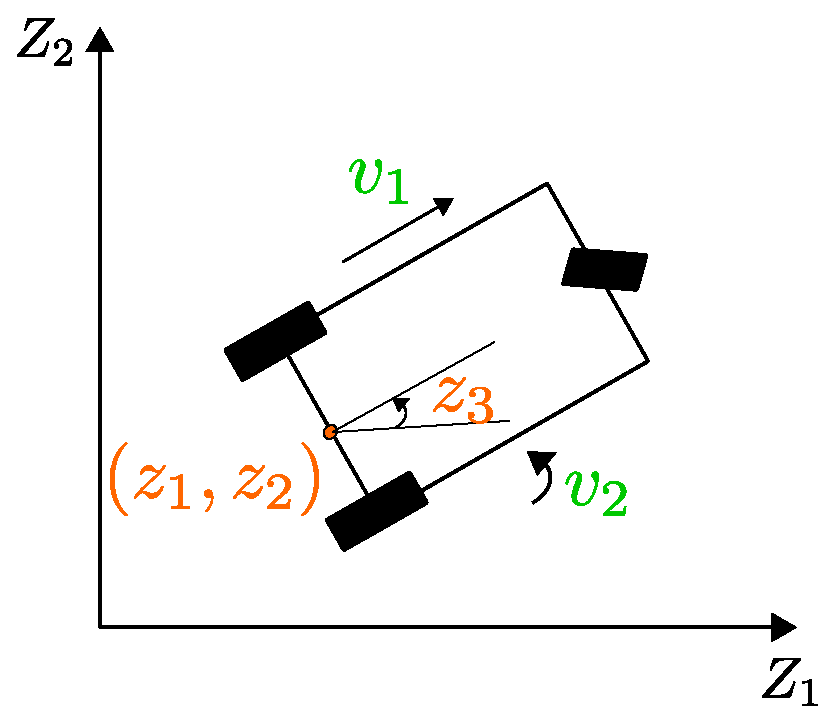
\includegraphics[width=0.4\linewidth]{bild/modul/Brocketts_Beispiel.eps}%6cm
		\caption[Skizze des mobilen Roboters mit einem Voreinrad.]{Skizze des mobilen Roboters mit einem Voreinrad. $(z_{1}, z_{2},z_{3})$ sind die Systemzustände und $(v_{1},v_{2})$ sind die Systemeingänge.}
		\label{fig:Brocketts_Doppelintegrator}
	\end{figure}  
	\begin{eqnarray}
	\dot{z}_{1} &=& v_{1}cos(z_{3})\notag\\
	\dot{z}_{2} &=& v_{1}sin(z_{3})\notag\\
	\dot{z}_{3} &=& v_{2}.
	\label{eq:Mobiler_Roboter_mit_Einrad}
	\end{eqnarray} 
	Das System hat $3$ Zustandskomponente: $z_{1}$ und $z_{2}$ steht jeweils für die Position des Punktes in der Mitte der der Hinterachse. $z_{3}$ ist der Winkel des Vorderrades mit der $z_{1}$-Achse. In dem System ergibt sich zwei Eingänge $v_{1}$ und $v_{2}$, die die Vorwärts- und Winkelgeschwindigkeit bedeuten.

	Mit der Rückkopplung der Systemzuständen und Eingängen \cite{liberzon2012switching}: 
	\begin{eqnarray}
	x_{1} &=& z_{1}\cos(z_{3}) + z_{2}\sin(z_{3})\notag\\
	x_{2} &=& z_{3}\notag\\
	x_{3} &=& 2\cdot(z_{1}\sin(z_{3})-z_{2}\cos(z_{3})) - z_{3}(z_{1}\cos(z_{3})+z_{2}\sin(z_{3}))\notag\\
	u_{1} &=& v_{2}\notag\\
	u_{2} &=& v_{1} - v_{2}(z_{1}\sin(z_{3})-z_{2}\cos(z_{3}))
	\label{eq:Mobiler_Roboter_mit_Einrad_Brockett_Doppelintegrator_Transformation}
	\end{eqnarray}
	kann Gln. \eqref{eq:Mobiler_Roboter_mit_Einrad} in der Form wie folgt transformiert werden:   
	\begin{eqnarray}
	\dot{x}_{1} &=& u_{1}\notag\\
	\dot{x}_{2} &=& u_{2}\notag\\
	\dot{x}_{3} &=& x_{2}u_{1}-x_{1}u_{2}.
	\label{eq:Brockett_Doppelintegrator}
	\end{eqnarray}
	Diese Zustandsfunktion beschreibt das berühmte System ``Brocketts nicht-holonomer Integrator''. 
  	Das Zustandsraummodell dieses Systems davon lautet:
	  \begin{eqnarray}
	  \dot{\vect{x}} = \begin{bmatrix}
	  0 & 0 & 0\\ 
	  0 & 0 & 0\\
	  -u_{2,e} & u_{1,e} & 0
	  \end{bmatrix}\vect{x} + \begin{bmatrix}
	  1 & 0\\
	  0 & 1\\
	  x_{2,e} & -x_{1,e} 
	  \end{bmatrix}\vect{u}
	  \label{eq:Brockett_doppel_Sytemzustand}
	  \end{eqnarray}
  	Ersetzt man den linken Teil von Gln. \eqref{eq:Brockett_doppel_Sytemzustand} mit $\vect{0}$, erhält man die Ruhelagen dieses Systems: $(x_{1},x_{2},x_{3})=(c_{1},c_{2},c_{3})$ beliebig mit $u_{1}=u_{2}=0$. Das heißt, die Eigenwerte des Systems sind alle $0$, \textbf{ohne} positive Realteile zu verfügen. Die Brockett $1.$ Bedingung ist nicht verletzt.
   
  	Zur Konstruktiven der $2.$ Bedingung kann man einen Regler wie folgt entwerfen:
	  \begin{eqnarray}
	  	\begin{pmatrix}
	  	0\\ 
	  	0\\ 
	  	0
	  	\end{pmatrix}\xrightarrow[Phase-\textrm{I}, 1s]{\vect{u}_{1}}\begin{pmatrix}
	  	\ast \\ 
	  	\ast \\ 
	  	0
	  	\end{pmatrix}\xrightarrow[Phase-\textrm{II}, 1s]{\vect{u}_{2}}\begin{pmatrix}
	  	\ast \\ 
	  	\ast \\ 
	  	\omega 
	  	\end{pmatrix}\xrightarrow[Phase-\textrm{III}, 1s]{\vect{u}_{3}}\begin{pmatrix}
	  	\alpha\\ 
	  	\beta\\ 
	  	\gamma
	  	\end{pmatrix}
	  \end{eqnarray}
  	mit $\vect{u}_{1}, \vect{u}_{2}, \vect{u}_{3}$ drei Regelgesetzen (nicht Regler $u_{1}$ oder $u_{2}$ in Gl. \eqref{eq:Brockett_Doppelintegrator}) in drei Phasen (Nimmt man an, dass jede Phase $1s$ dauert.) und $\begin{pmatrix}
   \ast  & \ast  & 0
   \end{pmatrix}^{T}, \begin{pmatrix}
   \ast  & \ast  & \omega
   \end{pmatrix}^{T}$ zwei Hilfspunkte. Es ist schon bekannt, wenn eine Trajektorie von Punkt A nach B existiert, gibt es unbedingt eine umgekehrte Trajektorie von B nach A. Ohne die Einfachheit zu verlieren, konstruiert man hier die Trajektorie von der Ursprung $(\vect{x}=\vect{0})$ nach einem beliebigen Punkt $(\vect{x}_{end}=(\alpha,\beta,\gamma))$.  In Phase-$\textrm{I}$ soll der Zustandsvektor mit $\vect{u}_{1}$ aus der Ruhelage zu den Hilfspunkt $1$ gehen, dann soll er in $1s$ zu den Hilfpunkt $2$ erreichen. Und endlich soll er mittels $\vect{u}_{3}$ am beliebigen Punkt $\begin{pmatrix}
   \alpha  & \beta  &\gamma
   \end{pmatrix}^{T}$ stoppen können. 
  
   EinAnsatz mit Konstanten $u_{1}$ und $u_{2}$ wie:
   \begin{eqnarray}
   Phase-\textrm{I}:~u_{1} = a_{1}, u_{2} = b_{1}\notag\\
   Phase-\textrm{II}:~u_{1} = a_{2}, u_{2} = b_{2}\notag\\
   Phase-\textrm{III}:~u_{1} = a_{3}, u_{2} = b_{3}
   \end{eqnarray}
   ist genügend, die obere Trajektorienbedingungen zu erfüllen.
   Zum Zeitpunkt $t=3s$ gilt:
   \begin{eqnarray}
   x_{1}(3s) &=& a_{1}  +a_{2} + a_{3}\notag\\
   x_{2}(3s) &=& b_{1} + b_{2} + b_{3}\notag\\
   x_{3}(3s) &=& (b_{1} + b_{2})a_{3} - (a_{1} + a_{2})b_{3} + b_{1}a_{2} - b_{2}a_{1}.
   \end{eqnarray}
   Mit diesem Regelgesetz kann das System in $3s$ irgendwo außerhalb dem Punkt $(\alpha=0,\beta=0,\gamma=0)^{T}$ ankommen. Um diesen Endzustand erreichen zu können, muss $\omega$ in Hilfspunkt $2$ äquivalent zu $\gamma$ sein. Das ist die einzelne Anforderung von der Größe von $(\alpha,\beta,\gamma)$. Deswegen kann das System mit diesem Regelgesetz die Brockett $2.$ Bedingung erfüllen.
  
   Letztlich wird die 3. Bedingung überprüft. Setzt man voraus, dass $\vect{\epsilon}$ in der offenen Menge $M=B(\vect{x},\varepsilon)$ liegt, dann gilt 
   \begin{eqnarray}
   \vect{\epsilon}  = \begin{bmatrix}
   \epsilon _{1}\\ \epsilon_{2} \\ \epsilon_{3}
   \end{bmatrix} = 
   \begin{bmatrix}
   u_{1\epsilon }\\ u_{2\epsilon } \\ x_{2\epsilon}u_{1\epsilon}- x_{1\epsilon}u_{2\epsilon}
   \end{bmatrix}.
   \label{eq:doppel_Brockett}
   \end{eqnarray}
  
   Die Menge $M$ enthält einen Punkt $\vect{x}_{um}=(0,0,\delta)$ mit $\delta<\varepsilon$. Offensichtlich ist es unmöglich, das Bild der Abbildung $\Gamma: \left ( \vect{x},u \right ) \mapsto \vect{f}\left ( \vect{x},u \right )$ einen Wert gleich $\vect{x}_{um}$ zu sein. Nämlich ist $\Gamma$ nicht surjektiv zu $M$.
  
   D.h. das System verletzt die Brockett Bedingung. Deswegen existiert kein stetig differenzierbarer Regelgesetz, mit dem der Ursprung asymptotisch stabil ist.
\end{beispiel}
 
Fazit: In diesem Kapitel wurde das Brockett Theorem für die Überprüfung der Existenz einer asymptotischen stabilen Ruhelage in einem nichtlinearen System mittels eines stetigen differenzierbaren Regelgesetz vorgestellt. In den Literatur \cite{brockett1983asymptotic} lieferte Brockett schon einen Beweis für das Theorem, der aber für die Leser ohne tiefen Kenntnisse der Topologie  vergleichsweise schwer verständlich ist. Daher erklärt die Autorin hier den Beweisvorgang mit einfacheren Worten. Ein einfaches nichtholonom Doppelintegrator System wurde als Beispiel für die Anwendung der Brockett-Bedingung diskutiert.
%------------------------------------------------------------------------------
\ifpdf
\graphicspath{{bild/}}
%{80_Bilder/PDF/}
%{80_Bilder/}}
\else
\graphicspath{%{80_Bilder/EPS/}
	%{80_Bilder/}
	{bild/}}
\fi
%%%%%%%%%%%%%%%%%%%%%%%%%%%%%%%%%%%%%%%%%%%%%%%%%%%%%%%%%%%%%%%%%%%%%%
%%%%%%%%%%%%%%%%%%%%%%%%%%%%%%%%%%%%%%%%%%%%%%%%%%%%%%%%%%%%%%%%%%%%%%


\chapter{Trajektorieplanung durch Lösung einer Randwertaufgabe}
\label{ch:Trajektorieplanung_durch_Lösung_einer_Randwertaufgabe}

Dieses Kapitel befasst sich mit der Trajektorieplanung von dem nichtlinearen System mittels des Python-Pakets \emph{PyTrajectory}. Im ersten Abschnitt geht es um die Vorstellung der allgemeinen Idee und den Algorithmen für die Trajektorieplanung mit dem Paket. In Abschnitt \ref{Erweiterung_der_Funktion_von_PyTrajectory} werden einige Probleme mit den Lösungen aus den Algorithmen diskutiert. Die simulierten Ergebnisse verschiedener Systeme werden auch in diesem Abschnitt vorgestellt.


\section{Grundlage zum Entwurf der Trajektorieplanung}
\label{Grundlage_zum_Entwurf_der_Trajektorieplanung}
\emph{PyTrajectory} ist ein Python Paket zum Trajektorien-Entwurf mit gegebenen Randwertbedingungen (Anfangs- und Endwerte der Systemzuständen sowie Eingängen) für nichtlineare Systeme. Hier wird die Grundlage über Trajektorienplanung grundsätzlich vorgestellt. Für weitere Informationen steht die Dokumentation der Software \cite{PyTra} zur Verfügung.
%%%%%%%%%%%%%%%%%%%%%%%%%%%%%%%%%%%%
\subsection{Kollokationsverfahren}
\label{Kollokationsverfahren}
Gesucht ist die Lösung $t\mapsto\vect{u}(t)$ des Randwertproblems:
\begin{eqnarray}
\vect{f}(\vect{x}(t), \vect{u}(t)) - \dot{\vect{x}} &=& \vect{0}, ~~t\in [0,T]
\label{eq:Kollocationverfahren}
\end{eqnarray}
mit dem Anfangswert $\vect{x}_{0} = \vect{X}_{a}$, Endwert $\vect{x}_{T} = \vect{X}_{b}$ an. $\dot{\vect{x}}$ ist die Ableitung nach der Zeit $t$, $\vect{X}_{a}\in \Reals^{n}, \vect{X}_{b}\in \Reals^{n}$ sind gegeben und $\vect{u}: \Reals\mapsto \Reals^{m}$ bezeichnet das gesuchte Eingangssignal. 

Das Zeitintervall $I = [0,T] $ kann wie Abb. \ref{fig:Collocation} unterteilt werden:
\begin{figure}
	\centering
	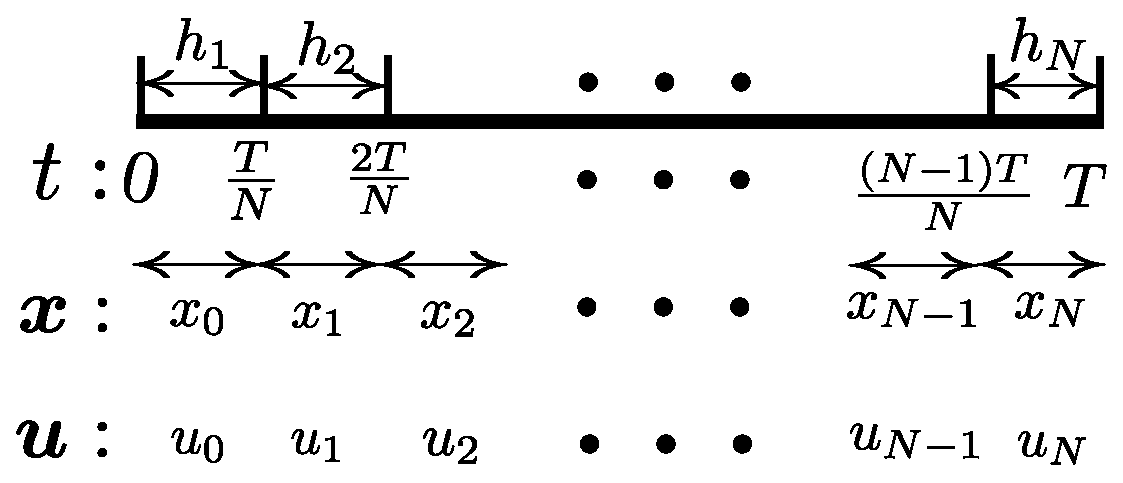
\includegraphics[width=7cm]{bild/modul/Collocation.eps}
	\caption[Kollokationsabschnitte $h_{i}$ und Kollokationspunkte $\vect{x}_{i}$, $\vect{u}_{i}$.]{Kollokationsabschnitte $h_{i}$ und Kollokationspunkte $\vect{x}_{i}$, $\vect{u}_{i}$: für jeden Abschnitt ist die Darstellung von $\vect{x}$ und $\vect{u}$ jeweils ein Polynom über $t$. Die Anzahlen der Splineabschnitte von $\vect{x}$ und $\vect{u}$ brauchen nicht äquivalent zu sein. (In dieser Abbildung sind sie als spezieller Fall gleich.)}
	\label{fig:Collocation}
\end{figure} 
 
Das Intervall $[0,T]$ wird in $N$ Teile mit gleichen Abstand eingeteilt ($h_{1} = h_{2} = \cdots = h_{N} = \frac{T}{N}$). Für jeden Abschnitt nimmt man eine Polynomfunktion dritten Grades jeweils für $\vect{x}$ und $\vect{u}$ an:
\begin{eqnarray}
\vect{S}_{x,i}(\vect{c},t) = \vect{x}_{i} &=& c_{xji0}+c_{xji1}\cdot (t-\frac{iT}{N_{x}}) + c_{xji2}\cdot (t-\frac{iT}{N_{x}})^{2} \notag\\&+& c_{xji3}\cdot (t-\frac{iT}{N_{x}})^{3}, ~~\scriptstyle{t\in [\frac{iT}{N_{x}}, \frac{(i+1)T}{N_{x}}),~~i= 0\cdots N_{x}-1, ~~j = 1\cdots n}\notag\\ 
\vect{S}_{u,i}(\vect{c},t) = \vect{u}_{i} &=& c_{uji0}+c_{uji1}\cdot (t-\frac{iT}{N_{u}}) + c_{uji2}\cdot (t-\frac{iT}{N_{u}})^{2} \notag\\&+& c_{uji3}\cdot (t-\frac{iT}{N_{u}})^{3}, ~~\scriptstyle{t\in [\frac{iT}{N_{u}}, \frac{(i+1)T}{N_{u}} ),~~i= 0\cdots N_{u}-1, ~~j = 1\cdots m}
\label{eq:form_von_Polynom_u_und_x}
\end{eqnarray}
Der Index $i$ und $j$ steht jeweils für den $i$-ten Abschnitt in Abb. \ref{fig:Collocation} und die $(j+1)$-te Komponente von $x$ bzw. $u$ (Da $\vect{x}/\vect{u}$ Vektor ist). $\vect{c}$ bedeutet Koeffizient der Polynomen. Es gibt insgesamt $4\cdot (N_{x}\cdot n + N_{u}\cdot m)$ Koeffizienten von $\vect{x}$ und $\vect{u}$ in $(N_{x}\cdot n + N_{u}\cdot m)$ kubischen Polynomfunktionen. 
 
Jetzt berücksichtigt man die Stetigkeit von $\vect{S}$. Die Polynomfunktionen sollen an der Abschnittsgrenzen zweimal stetig differenzierbar sein. Mit anderen Worten erfüllen sie in jeder Übergangsstelle folgende Formel:
\begin{eqnarray}
\vect{S}_{x/u,i}\left(\vect{c},t = \frac{iT}{N_{x}/N_{u}}\right ) &=& \vect{S}_{x/u,i+1}\left((\vect{c},t = \frac{iT}{N_{x}/N_{u}}\right )~~~~~~\text{(0.~Ableitung~stetig)}\notag\\
\dot{\vect{S}}_{x/u,i}\left(\vect{c},t = \frac{iT}{N_{x}/N_{u}}\right ) &=& \dot{\vect{S}}_{x/u,i+1}\left((\vect{c},t = \frac{iT}{N_{x}/N_{u}}\right )~~~~~~\text{(1.~Ableitung~stetig)}\notag\\
\ddot{\vect{S}}_{x/u,i}\left((\vect{c},t = \frac{iT}{N_{x}/N_{u}}\right ) &=& \ddot{\vect{S}}_{x/u,i+1}\left((\vect{c},t = \frac{iT}{N_{x}/N_{u}}\right )~~~~~~\text{(2.~Ableitung~stetig)}.\notag\\
\end{eqnarray}
Deswegen gibt es insgesamt $3((N_{x}-1)\cdot n + (N_{u}-1)\cdot m)$ Funktionen mit $(N-1)$ der Anzahl der Übergangsstellen. Mit dem Anfangs- und Endwert von $\vect{x}$ und $\vect{u}$ (insgesamt $2\cdot (n+m)$) werden $N_{cf} = (n\cdot (N_{x}+1) + m \cdot (N_{u}+1))$ freie Parameter $\vect{c}_{f}$ für Koeffizienten sichergestellt. Die anderen $N_{ca} = (n\cdot (3N_{x}-1) + m\cdot (3N_{u}-1))$ Parameter von Polynomen $\vect{c}_{a}$ hängen durch die obengenannten Funktionen von $\vect{c}_{f}$ ab.

Der freie Parametervektor $\vect{c}_{f}$ kann durch \eqref{eq:Kollocationverfahren} bestimmt werden. Dazu setzt man die Polynomform von $\vect{x}$ und $\vect{u}$ in Gl. \eqref{eq:Kollocationverfahren} ein und wählt man $(N_{t}+1)$ beliebigen Zeitpunkten\footnote{In \emph{PyTrajectory} wählt man Zeitpunkte mit festen Abstand: $t_{k} = \frac{kT}{N_{t}}, k = 0 \cdots N_{t}$.}:
\begin{eqnarray}
\vect{F\left (  \vect{c}_{f} \right )}&=&\begin{pmatrix}
\vect{f}\left ( \vect{S}_{x}\left ( \vect{c}_{f},t_{0} \right ), \vect{S}_{u}\left ( \vect{c}_{f},t_{0} \right ) \right )-\dot{\vect{S}}_{x}\left ( \vect{c}_f,t_{0} \right ) = \vect{0}\\
\vect{f}\left ( \vect{S}_{x}\left ( \vect{c}_{f},t_{1} \right ), \vect{S}_{u}\left ( \vect{c}_{f},t_{1} \right ) \right )-\dot{\vect{S}}_{x}\left ( \vect{c}_f,t_{1} \right ) = \vect{0}\\
\cdots  
\\
\vect{f}\left ( \vect{S}_{x}\left ( \vect{c}_{f},t_{N_{t}} \right ), \vect{S}_{u}\left ( \vect{c}_{f},t_{N_{t}} \right ) \right )-\dot{\vect{S}}_{x}\left ( \vect{c}_f,t_{N_{t}} \right ) = \vect{0}
\end{pmatrix}=\vect{0}\\ ~\text{mit}~~\vect{f}&:& \Reals^{N_{cf}}\mapsto \Reals^{n}\notag.
\label{eq:Gesamte_Funktion_von_KollocationVerfahren}
\end{eqnarray}
Die Dimension der unabhängigen Variablen $\vect{c}_{f}$ ist $N_{cf}$ und die Dimension von $\vect{F\left (  \vect{c}_{f} \right )}$ ist $n\cdot(N_{t}+1)$. Wenn die Anzahl der Variablen gleich oder größer als der Funktionen ist, wird mindestens eine exakte Lösung ausgerechnet. Das sichert die Funktionswerte zu den $(N_{t}+1)$ Zeitpunkten. Aber die Werte zu anderen Zeitpunkten können nicht garantiert werden.  Wie Abb. \ref{fig:Collocation_overdetermined} zeigt, liegt die Kurve $1$ zu den $(N_{t}+1)$ Zeitpunkten gerade auf der Achse, aber zu anderen Punkten liegt sie sehr weit von der Achse. Dagegen erhält die Kurve $2$ zu jedem Zeitpunkt zwar keine exakte Lösung, aber die Norm ist sehr klein. Deswegen sollte man für das Kollocationsverfahren eine überbestimmte Funktion auswählen, nämlich $n\cdot(N_{t}+1)>(n\cdot (N_{x}+1) + m \cdot (N_{u}+1))$.
\begin{figure}
	\centering
	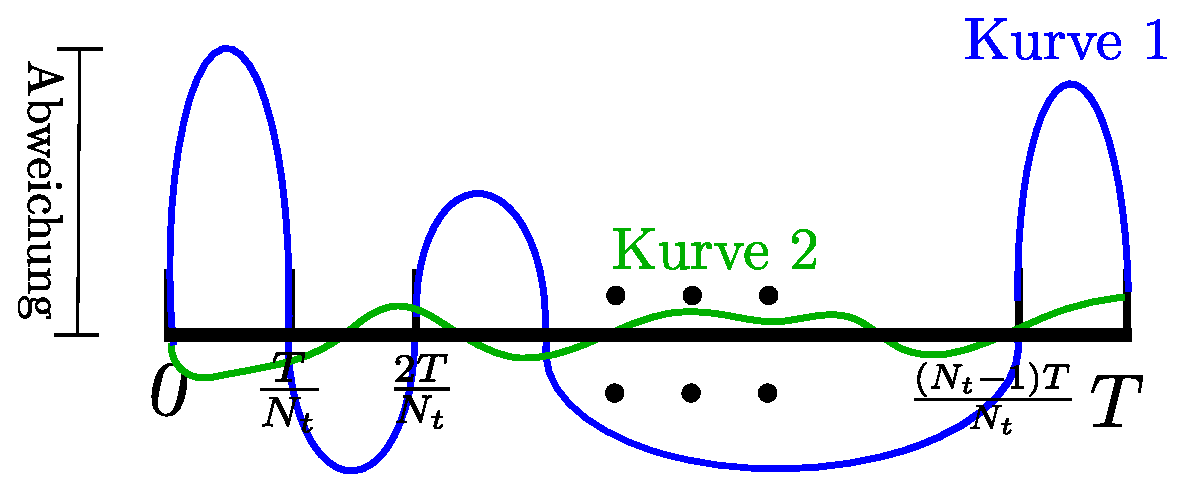
\includegraphics[width=8cm]{bild/modul/Collocation_overdetermined.eps}
	\caption[2 Trajektorienfälle von beispielsweise dem Systemzustand]{2 Trajektorienfälle von beispielsweise dem Systemzustand: aus Grund der Einfachheit ist $dim(\vect{x})=1$ gewählt. Die $y$-Achse ist die Abweichung zwischen der approximierten Lösung und dem idealen Fall. Zwar geht die Kurve $1$ zu den gewählten Zeitpunkten die $x$-Achse durch, aber sie hat eine viel größer Abweichung zu anderen Punkten als Kurve $2$.}
	\label{fig:Collocation_overdetermined}
\end{figure}  

Jetzt stellt sich die Frage: wie kann man eine optimale approximierte Lösung von der überdeterminierte Funktion (Gl. \eqref{eq:Gesamte_Funktion_von_KollocationVerfahren}) bestimmen? Das wird in nächsten Abschnitt beantwortet.
%%%%%%%%%%%%%%%%%%%%%%%%%%%%%%%%%%%%%%%%%%%%%%%%%%%%%%%%%
\subsection{Methode zur Lösung des Quadratmittelproblems}
\label{Methode_zur_Lösung_des_Quadratmittelproblems}
Das Quadratmittelproblem einer Funktionsvektor ist wie folgt definiert \cite{knorrenschild2017numerische}:
\begin{definition}[Quadratmittelproblem]
Gegeben ist ein Funktionsvektor\footnote{$n$ und $m$ hier sind anders wie die Dimensionen von $\vect{x}$ und $\vect{u}$ in letztem Abschnitt. $\vect{x}$ verweist nur die erforderlichen Parameter.}${\vect{F\left (\vect{x}\right )}}: \Reals^{n}\to \Reals^{m}$. Ein Vektor ${\vect{x}_{\ast}}$ ist zu finden, sodass die euklidische Norm des Funktionsvektors (oder: das ``zugehörige Fehlerfunktional'') minimiert wird:
\begin{eqnarray}
{\vect{x}_{\ast}} = \mathop {\argmin }\limits_{\vect{x}}\left | {\vect{F}}\left ( {\vect{x}} \right ) \right |_{2}^{2} = \mathop {\argmin }\limits_{\vect{x}}\left ( \sum_{i=1}^{m}\left ( f_{i}\left ( \vect{x} \right ) \right )^{2}\right )
\label{Def_LSP}\notag\\
\end{eqnarray}
mit $f_{i}: \Reals^{n}\to \Reals^{1}$. $\vect{x}_{\ast}$ hießt auch der stationäre Punkt.
\end{definition}
\subsubsection{Gauß-Newton-Verfahren}\label{Gauß-Newton-Verfahren}
%%%%%%%%%%%%%%%%%%%%%%%%%%%%%%%%%
Ein solches Quadratmittelproblem kann man mit verschieden Verfahren lösen. Eine typische Methode ist das Gauß-Newton-Verfahren (GN-Verfahren), das durch die lineare Approximation des nichtlinearen Problems löst. Mit der Ableitung erster Ordnung der Funktion $\vect{F(\vect{x})}$ konvergiert das Iterationsverfahren mit linearer Konvergenzordnung\footnote{Linear Konvergenzordnung bedeutet, dass $\norm{\vect{x}_{k+1} -\vect{x}_{\ast}} \leqslant \alpha \norm{\vect{x}_{k}-\vect{x}_{\ast}}$ mit $0 \leqslant \alpha \leqslant 1$.}. Im Folgenden geht die Methode mit der Taylorentwicklung von $\vect{F}$ und $f$ aus \cite{madsen2004methods}:
\begin{equation}
\begin{aligned}
f\left ( \vect{x}+\vect{h} \right ) &= f\left ( \vect{x} \right ) + f'\left ( \vect{x} \right )\cdot \vect{h} \overset{f' = \matr{J}}{=} f\left ( \vect{x} \right ) + \matr{J}\left ( \vect{x} \right )\cdot \vect{h} + o\left ( \vect{h}^{2} \right )\\
\vect{F}\left ( \vect{x}+\vect{h} \right ) &= f\left ( \vect{x}+\vect{h} \right )^ \mathrm{ T }\cdot f\left ( \vect{x}+\vect{h} \right )\approx \left ( f+\matr{J}\vect{h} \right )^ \mathrm{ T }\left ( f+\matr{J}\vect{h} \right )\\ &= f^ \mathrm{ T }f+2\vect{h}^ \mathrm{ T }\matr{J}^ \mathrm{ T }f + \vect{h}^ \mathrm{ T }\matr{J}^ \mathrm{ T }\matr{J}\vect{h} := \vect{G}\left ( \vect{h} \right ).\label{eq:Taylorentwicklung_von_GN_Verfahren}
\end{aligned}
\end{equation}
Das Symbol $\matr{J}$ steht für die Jacobi-Matrix. Nach der Ableitung des vorletzten Terms erhält man die 1. und 2. Ableitung von $\vect{G}$ bezüglich $\vect{h}$:
\begin{eqnarray}
\vect{G}'\left ( \vect{h} \right )  &=& 2\matr{J}^\mathrm{T}f + 2\matr{J}^\mathrm{T}\matr{J}\vect{h}\label{eq:G_1}\\
\vect{G}''\left ( \vect{h} \right ) &=& 2\matr{J}^\mathrm{T}\matr{J}.\label{eq:G_2}
\end{eqnarray}
Es wir angenommen, dass $\vect{G}''$ positiv definit ist\footnote{Das ist ein Nachteil von Gauß-Newton-Verfahren. Die Positivdefinitkeit kann nicht immer gesichert werden.}. Man definiert hier die Schrittweite $h=h_{\ast}$ als lokaler Minimum, wenn $\vect{G}'\left (\vect{h}_{\ast} \right ) = \vect{0}$ ist. Zur Berechnung von $\vect{h}_{\ast}$ wird Gl. \eqref{eq:G_1} gleich $0$ gesetzt:
\begin{equation}
\left ( \matr{J}^\mathrm{T} \matr{J} \right ) \cdot \vect{h}_{\ast}  = -\matr{J}^\mathrm{T}f.\label{eq:cal_NW_hs}
\end{equation}
Der stationäre Punkt $\vect{x}_{\ast}$ wird aus der vorherige Punkt $\vect{x_{\ast-1}}$ und $\vect{h}_{\ast}$ berechnet:
\begin{equation}
\vect{x}_{\ast} = \vect{x_{\ast-1}} + \vect{h}_{\ast} = \vect{x_{\ast-1}} - \left ( \matr{J}^\mathrm{T} \matr{J} \right )^\mathrm{-1} \cdot \matr{J}^\mathrm{T}f.\label{eq:newton-xs}
\end{equation} 
Neben der möglichen Nichtexistenz der inversen Matrix gibt es auch eine Beschränkung: mit der $\vect{x}_{\ast}$ durch das GN-Verfahren nicht gefunden kann, wenn der Anfangsschätzwert $\vect{x}_{0}$ nicht in der Näher von $\vect{x}_{\ast}$ liegt. Daher wird in nächsten Abschnitt eine andere Methode vorgestellt, damit man die obige Probleme vermeiden kann. 
\subsubsection{Levenberg-Marquardt-Algorithmus}
\label{Levenberg-Marquadt-Algorithmus}
%%%%%%%%%%%%%%%%%%%%%%%%%%%%%%%%%%%%%%%
Der nach Kenneth Levenberg und Donald Marquardt benannte Algorithmus ist tatsächlich eine Kombination von Methode des steilsten Abstiegs und Gauß-Newton-Verfahrens. Gl. \eqref{eq:LM_cal_hs} zeigt die detaillierte Form von Schrittweite $\vect{h}$ in LM-Algorithmus \cite{von2015einfuhrung}\cite{madsen2004methods}:
\begin{equation}
\left ( \matr{J}^\mathrm{T} \matr{J} + \mu\matr{I}\right ) \cdot \vect{h}  = -\matr{J}^\mathrm{T}f.
\label{eq:LM_cal_hs}
\end{equation}
$\matr{I}$ ist die Einheitsmatrix, $\mu$ ist ein ``Dämpfungsparameter''. Aufgrund der Existenz des Dämpfungparameters ist die Positivdefinitheit der Matrix $\matr{J}^\mathrm{T} \matr{J} + \mu\matr{I}$ gesichert. Falls $\mu$ groß ist (das passiert am Anfang der Iteration), ist die Funktion von der Schrittweite ähnlich wie Methode des steilsten Abstiegs, damit die Funktion bei $\vect{x}$ weit von Zielpunkt schnell konvergiert. Andernfalls verhält sich der LM-Algorithmus bei kleinem $\mu$ oder in der Umgebung von $\vect{x}_{\ast}$ wie NM-Verfahren aus. Das heißt, in den letzten Schritten konvergiert die Funktion auch schnell.

Ein wichtiger Teil für LM-Algorithmus ist die Bestimmung von Dämpfungsparameter $\mu$. Der Ausgangspunkt davon ist die Größe der Variable \emph{Verstärkungsverhältnis $\rho$}, die durch die Relation von der aktuellen Abnehme des nichtlinearen Systems in einem Schritt und der vorhergesagten Abnehme des linearisierten Systems definiert wird:  
\begin{eqnarray}
	\rho  = \frac{\left \|\vect{F}\left ( \vect{x} \right )\right \|^{2}-\left \| \vect{F}\left ( \vect{x}+\vect{h} \right )\right \|^{2}}{\left \| \vect{G}\left ( \vect{0} \right )\right \|^{2}-\left \| \vect{G}\left ( \vect{h} \right )\right \|^{2}} = \frac{\Delta F}{\Delta G}.
\label{eq:LM-Methode-rho}
\end{eqnarray}
Da $\vect{h}$ in die Richtung mit einer sinkenden Norm von $\vect{G}$ zeigt, soll der Wert von $\rho$ größer als $0$ sein. Wenn $\rho$ sehr klein oder $\Delta G$ viel größer als $\Delta F$ ist, ist der vorherige Schritt $\vect{h} = \min_{\vect{h}}{(\vect{G}(\vect{h}) + \frac{1}{2}\mu \vect{h}^{T}\cdot \vect{h})} $ zu groß und er muss im nächsten Schritt verkleinert werden. Das heißt, der Wert von $\mu$ muss vergrößert werden. Anderenfalls muss $\mu$ verkleinert werden, wenn der vorherige $\vect{h}$ zu klein (sonst kostet es mehrere Zeit, eine Lösung zu finden) ist. Ein typischer Entwurf von $\rho$ sieht wie folgendem Algorithmus:
\begin{algorithmic}
	%\centering
	\If {$\rho < 0.2$}
	\State $\mu_{new}: = \mu_{old} *2 $
	\ElsIf {$\rho > 0.8$}
	\State $\mu_{new}: = \mu_{old} / 2$
	\Else
	\State $\mu_{new} : = \mu_{old} $
	\EndIf
\label{Ag:dampfung_parameter}
\end{algorithmic}
                              
Setzt man Gl. \eqref{eq:Gesamte_Funktion_von_KollocationVerfahren} in Gl. \eqref{eq:LM_cal_hs} ein, ersetzt der Vektor $\vect{F(\vect{c}_{f})}$ hier $f$ und die freien Parameter $\vect{c}_{f}$ hier $\vect{x}$. Die Jacobi-Matrix $\vect{J}$ ist die Ableitungsmatrix von $\vect{F(\vect{c}_{f})}$ nach $\vect{c}_{f}$. Mit dem LM-Algorithmus wird eine optimale approximierte Lösung von $\vect{c}_{f}$ ausgerechnet. 

Nach der Iteration erhält man die optimalen freien Parameter, damit werden die Trajektorie von $\vect{u}(t)$ und $\vect{x}_{sp}(t)$ als Form der kubischen Polynom dargestellt wie Gl. \eqref{eq:form_von_Polynom_u_und_x}. Setzt man $\vect{u}(t)$ in den Zustandsgleichungen ein, wird auch ein $\vect{x}_{sim}(t)$ durch die Integration erstellt. Wenn die Abweichungen $1.)$ zwischen $\vect{x}_{sp}(t)$ und $\vect{x}_{sim}(t)$ und $2.)$ zwischen gegebenen Randwerte von $\vect{x}$ und $\vect{x}_{0}$, $\vect{x}_{T}$ unter den voraus gelieferten Beschränkungen nicht erfüllt werden, wird das System nochmal mit einer höheren Anzahl an Splineabschnitten gerechnet. Dieser Vorgang wird solange wiederholt, bis eine approximierte Lösung gefunden werden kann\footnote{Dieser Iterationsvorgang wird unter ``Hauptiteration'' genannt. Anders als die Iteration innerhalb des LM-Verfahrens (als Nebeniteration genannt)\label{Nebeniteraion} ist der Parameterwert nach einer Hauptiteration schon die optimale Lösung von LM-Verfahren, der aber die erforderte minimale Abweichung zwischen dem Soll- und Istendwert des Zustände überschreitet. Ein erneuter Iteraionsvorgang mit vergrößerten Anzahl der Splineabschnitte ist deswegen nötig.}.

Als Schluss dieses Abschnitts wird ein Beispiel mit \emph{PyTrajectory} gerechnet.

\begin{beispiel}[Einfacher Doppelintegrator mit \emph{PyTrajectory}]\label{bp:Dooelintegrator_ori}
 	Betracht man einen auf der X-Achse laufenden Wagen mit zwei Zustandskomponenten: die Verschiebung $x_{1}$ und die Geschwindigkeit $x_{2}$. Eine aufgeprägte Kraft wirkt auf den Wagen ein. Die Beschleunigung gilt als Systemeingang $u$. Die Systemgleichung lautet:
 	\begin{eqnarray}
 	\dot{x}_{1} &=& x_{2}\notag\\
 	\dot{x}_{2} &=& u.
 	\label{eq:Doppelintegrator}
 	\end{eqnarray}
 	
	Es sei gefordert, dass der Wagen sich von $0$ bis zu $1m$ bewegt und am Anfang und Ende in Ruhe ist. Mit anderen Worten ist der Anfangs- und Endwert von $x_{1}$ und $x_{2}$ jeweils ($0$,$1$) sowie ($0$,$0$). Die feste Überführungszeit ist $1$ Sekunde. 
	
	Die Anfangswerte der Parameter von dem \emph{PyTrajectory} ist wie folgt eingestellt: die Anfangsschätzwerte der freien Parameter für die Polynome $\vect{x}$ und $u$ als Form der Gl. \eqref{eq:form_von_Polynom_u_und_x} sind alle $0.1$, die Anfangszahl der Splineabschnitte für beide $\vect{x}$ und $u$ ist $2$. Falls nötig muss die Anzahl in dem nächsten Iteration verdoppeln.
	
	Abb. \ref{fig:Doppelintegrator_ohne_k_x} und Abb. \ref{fig:Doppelintegrator_ohne_k_u} zeigt die Simulationsergebnisse des Systems. Das System benötigt zwei Iterationen (nämlich endlich $4$ Spline-Abschnitte), um eine optimale Lösung von den freien Parameter $\vect{c}_{f}$ zu finden. Unter der Wirkung eines ungefähr sinusförmigen Eingangs mit maximal $6m/s^{2}$ läuft der Wagen entlang dem geplanten Weg. Das heißt, der Wagen beschleunigt sich in die ersten Halbzeit ($0.5s$), und nach der Erreichung der maximale Geschwindigkeit (circa $1.8m/s$) bremst er bis zum Stoppen.
	\begin{figure}[!h]
		\centering
		\includegraphics[width=0.7\linewidth]{bild/30_32/test0_ohne_k_ori_x.pdf} %13cm
		\caption[Trajektorie der Systemzustandskomponente $x_{1}$ und $x_{2}$ (Position und Geschwindigkeit).]{Trajektorie der Systemzustandskomponente $x_{1}$ und $x_{2}$ (Position und Geschwindigkeit). Die Überführungszeit ist fest: $1s$.}
		\label{fig:Doppelintegrator_ohne_k_x}
	\end{figure}
	
	
	
	\begin{figure}[!h]
		\centering
		\includegraphics[width=0.7\linewidth]{bild/30_32/test0_ohne_k_ori_u.pdf}%12cm
		\caption[Trajektorie des Systemeingangs $u_{1}$ (Wagenbeschleunigung).]{Trajektorie des Systemeingangs $u_{1}$ (Wagenbeschleunigung). Die Überführungszeit ist fest: $1s$.}
		\label{fig:Doppelintegrator_ohne_k_u}
	\end{figure}
\end{beispiel}

\section{Erweiterung der Funktion von PyTrajectory}
\label{Erweiterung_der_Funktion_von_PyTrajectory}
%%%%%%%%%%%%%%%%%%%%%%%%%%%%%%%%%%%%
Vor beginn der Arbeit war es möglich, eine Trajektorie von $\vect{u}$ und $\vect{x}$ eines Systems mithilfe des Pakets \emph{PyTrajectory} und der vom Nutzer voraus gelieferten Überführungszeit $T$ zu finden. Dabei könnten aber folgende Probleme auftreten: Einerseits wären die Systeme mit diesem $T$ nicht optimal (z.B. es bräuchte mehrmals Iterationen) , auf der anderen Seite kann bei manchen Systemen nur dann eine Trajektorie gefunden werden, wenn man zufällig die richtige Dauer gewählt hat. Deswegen liegt eine Aufgabe bei der Erweiterung der Funktion von PyTrajectory darin, eine geeignete Überführungszeit der Trajektorienplanung eines Systems ausrechnen zu lassen, anstatt sie vorgeben zu müssen.

\subsection{Optimale Überführungszeit}
\label{Optimale_Überführungszeit}
Es wird angestrebt, dass die Überführungszeit $T$ nicht vom Nutzer explizit vorgegeben wird, sondern anhand der Systemgleichungen mittels des Levenberg-Marquardt-Algorithmus automatisch ausgerechnet wird. Der Anfangspunkt ist die Ansetzung der Zeittransformation von $t = t$ zu $t = k\tau$, wobei $k$ ein zusätzlicher freier Parameter (ohne Einheit) ist. Dann folgt die Transformation:
\begin{eqnarray}
\dot{\vect{x}}_{\mathrm{ori}} &=& \frac{\mathrm{d} \vect{x}}{\mathrm{d} t} = \vect{f}\left ( \vect{x},t \right )\notag\\ %\label{eq:ori}\\
\dot{\vect{x}}_{\mathrm{new}} &=& \frac{\mathrm{d} \vect{x}}{\mathrm{d} \tau} = \frac{\mathrm{d} \vect{x}}{\mathrm{d} t}\cdot \frac{\mathrm{d} t}{\mathrm{d} \tau} = k\cdot \frac{\mathrm{d} \vect{x}}{\mathrm{d} t} = k\cdot \vect{f}(\vect{x},t) = \vect{f}_{\mathrm{new}}\left ( \vect{x},t,k \right ).\label{eq:mit_k}
\end{eqnarray}
Bei $k>1$ braucht das System mehr Zeit, um die Endposition zu erreichen und bei $k<1$ weniger. 

Nach der Implementierung in Python werden zwei Beispielsysteme damit getestet, um die Gültigkeit und Brauchbarkeit zu überprüfen. Für jedes Beispiel wird die unter der Berücksichtigung von Zeit entworfene Trajektorie (abgekürzt als ``Trajektorie mit k'') mit dem zum originalen System geeigneten Trajaktorie (Kurz als ``Trajektorie ohne k'') verglichen.
\begin{beispiel}[Doppelintegrator]\label{bp:Doppelintegrator_k}
	Die Ergebnisse für das System ``ohne k'' wurde schon im letzten Abschnitt vorgestellt. Die erweiterte Systemgleichung von dem System ``mit k'' sind:
	\begin{eqnarray}
	\dot{x}_{1} &=& k \cdot x_{2}\notag\\
	\dot{x}_{2} &=& k \cdot u.
	\label{eq:Doppelintegrator_mit_k}
	\end{eqnarray}
	
	Als Anfangswerte bleiben alle Parameter außer der Überführungszeit $T$ wie Bsp. \ref{bp:Dooelintegrator_ori} unverändert. $T$ hängt von der freie Variable $k$ mit dem Anfangsschätzwert $k_{0}=1.23$ ab.
	
	\textbf{Einstellung von Anfangswerte der freien Parameter $\vect{c}_{f}$ als $\vect{0.1}$:}~~Der Wagen bewegt noch von $0$ bis zu $1m$ und am Anfang und Ende bleibt er in Ruhe. Die Anfangsschätzwerte von $\vect{c}_{f}$ sind noch $0.1$, die Anzahl der Spline-Abschnitt am Beginn des Algorithmus und der entsprechende Multiplikator für die Iteration sind jeweils noch $2$. 
	
	Mehr als in der Randwertaufgabe-Lösung mit den originalen Systemgleichungen benötigt das erweitere System $4$ Hauptiterationen\footnote{Die Erklärung für Haupt- und Nebeniteration liest man \ref{Nebeniteraion}.} (also $16$ Spline-Abschnitte), um eine optimale Lösung von $\vect{c}_{f}$ zu finden.
	
	Aus Abb. \ref{fig:Doppelintegrator_mit_k_x} und Abb. \ref{fig:Doppelintegrator_mit_k_u} kann man erkennen, zwar die maximale Kraft und die Geschwindigkeit weit kleiner als die im originalen System sind, ist aber der Wert von $k$ ist hier ziemlich groß (ungefähr $1662,53$)! Der Wert von $k$ nimmt ab $1.23$ in jeden Iteration zu. Der Wagen in diesem Beispiel muss sich deshalb $1662s$ lang bewegen, bevor er in die Endposition ankommt. Das bedeutet, die Lösung von $k$ ist zwar \textbf{richtig} aber \textbf{nicht brauchbar}.
	\begin{figure}[!h]
		\centering
		\includegraphics[width=0.7\linewidth]{bild/30_32/test0_mit_k_ori_x.pdf}%13cm
		\caption[Verlauf der Systemzustände vom System \eqref{eq:Doppelintegrator_mit_k}.]{Verlauf der Systemzustände vom System\eqref{eq:Doppelintegrator_mit_k}. $x_{1}$ und $x_{2}$ stehen für Position und Geschwindigkeit. Anfangswerte der freien Spline-Parameter sind alle $0.1$. Die $x$-Achse steht nicht für die reale Überführungszeit, die tatsächlich $(1\cdot k)$ Sekunde dauert.}
		\label{fig:Doppelintegrator_mit_k_x}
	\end{figure}
	\begin{figure}[!h]
		\centering
		\includegraphics[width=0.7\linewidth]{bild/30_32/test0_mit_k_ori_u.pdf}%13cm
		\caption[Verlauf des Systemeingangs und die Veränderungskurve von $k$ vom System \eqref{eq:Doppelintegrator_mit_k}.]{Verlauf des Systemeingangs und die Veränderungskurve von $k$ vom System \eqref{eq:Doppelintegrator_mit_k}. $u_{1}$ stehen für Wagenbeschleunigung. Der Wert von $k$ steigt immer an. Anfangswerte der freien freien Parameter sind alle $0.1$. Es gibt insgesamt ungefähr $2000$ Nebeniterationen. Die ``Iteraion'' in der Abbildung von $k$ ist tatsächlich Nebeniteration (im Folgenden ebenso).}
		\label{fig:Doppelintegrator_mit_k_u}
	\end{figure}
	
	\textbf{Einstellung von Anfangswerte der freien Parameter $\vect{c}_{f}$ aus dem Simulationsergebnis der originalen Systemgleichungen:}~~Zur Verbesserung des Ergebnisses wird ein anderer Anfangswert für die Splineparameter gewählt. Statt aller Werte $0.1$ sind die freien Parameter jetzt gleich den Rechenergebnissen der Splineparameter nach der ersten Iteration in dem System ``ohne k''. Die Kurven in Abb. \ref{fig:Doppelintegrator_mit_k_x_aus} und \ref{fig:Doppelintegrator_mit_k_u_aus} sehen besser als in Abb. \ref{fig:Doppelintegrator_mit_k_x} und Abb. \ref{fig:Doppelintegrator_mit_k_u} aus. In dem ganzen Iterationsverlauf steigt der Wert von $k$ hauptsächlich mit $2$-mal Abstieg (bei der ersten und siebten Iteration). Im Vergleich zu dem Simulationsergebnis mit allen Anfangswerten $0.1$ braucht diese nur zwölf Nebeniterationen. Der Wagen stoppt zum Zeitpunkt $1.67$s. 
	
	\begin{figure}[!h]
		\centering
		\includegraphics[width=0.7\linewidth]{bild/30_32/test0_mit_k_Ite1_x.pdf}%13cm
		\caption[Trajektorie der Systemzustandskomponente vom System \eqref{eq:Doppelintegrator_mit_k}.]{Trajektorie der Systemzustandskomponente vom System \eqref{eq:Doppelintegrator_mit_k}. Anfangswerte von $\vect{c}_{f}$ sind aus den Ergebnissen von originalen Systemgleichungen (ohne k) gegeben.}
		\label{fig:Doppelintegrator_mit_k_x_aus}
	\end{figure}

	\begin{figure}[!h]
		\centering
		\includegraphics[width=0.7\linewidth]{bild/30_32/test0_mit_k_Ite1_u.pdf}%13cm
		\caption[Trajektorie des Systemeingangs vom System \eqref{eq:Doppelintegrator_mit_k}.]{Trajektorie des Systemeingangs vom System \eqref{eq:Doppelintegrator_mit_k}. Anfangswerte von $\vect{c}_{f}$ sind aus den Ergebnissen von originalen Systemgleichungen gegeben.}
		\label{fig:Doppelintegrator_mit_k_u_aus}
	\end{figure}
	
\end{beispiel}

Dieses Beispiel zeigt eine starke Abhängigkeit der Konvergenz des Levenberg-Marquardt-Algorithmus von den Anfangsschätzwerten. Wenn die Anfangsschätzwerte der Parameter zu weit von der unbekannten Minimalstelle vorgegeben werden, kann die Lösung des Quadratmittelproblems eines Regelsystems mittels LM-Algorithmus nicht konvergieren oder erreicht nur einen lokalen, nicht global optimierten Punkt.

Das folgende Beispiel stellt die Anwendung der LM-Methode in einem verbreiterten nichtlinearen System vor.

\begin{beispiel}[Inverses-Pendel-System]\label{bp:Inverses_Pendel_System}
	Abb. \ref{fig:Inverses-Pendel} zeigt das Schema des inversen Pendels. Der Pendelarm ist auf einem horizontal bewegten Wagen montiert. Der Wagen bringt daher eine horizontale Kraft auf das Pendel auf. Beim Aufprägen der Kraft ${F}$ auf den Wagen bewegt sich das Pendel von unten nach oben. Die instabile Ruhelage ist der Punkt, in dem das Pendel genau senkrecht zum Wagen steht und der Drehwinkel $180^{\circ}$ beträgt. Systemvariable in diesem Modell sind die Wagenposition ${x}_{1}$, dessen Geschwindigkeit ${x}_{2}$, der Pendeldrehwinkel ${x}_{3}$, die Drehgeschwindigkeit davon ${x}_{4}$. Der einzige Systemeingang ist die auf den Wagen aufgeprägte Kraft $u=f_{w}$.
	\begin{figure}
		\centering
		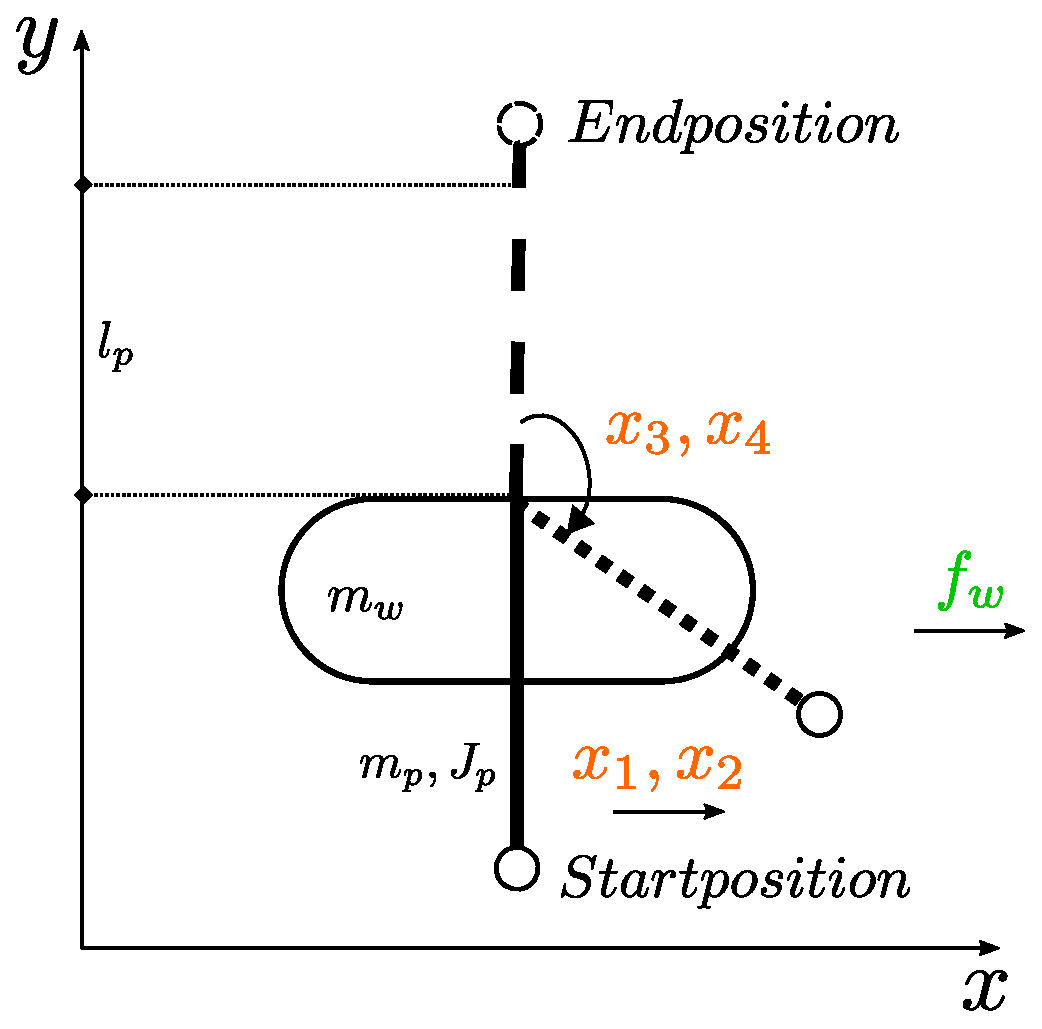
\includegraphics[width=6cm]{bild/modul/Inverses-Pendel.eps}
		\caption[Struktur des inversen Pendels.] {Struktur des inversen Pendels: in dem System gibt es vier Zustände ${x}_{1}$ bis ${x}_{4}$. Das Pendel bewegt sich von $180^{\circ}$ bis zur instabilen Ruhelage (nämlich vom ganz unten zu ganz oben). $m_{w}$ und $m_{p}$ sind jeweils die Masse des Wagens und des Pendels, $J_{p}$ ist das Trägheitsmoment und $l_{p}$ ist der Abstand zwischen dem Stützpunkt und dem Pendelschwerpunkt. Die Pfeile neben Zuständen geben die Vektorrichtung an. $x$ und $y$ sind Koordinatenachsen.}
		\label{fig:Inverses-Pendel}
	\end{figure}  

	Die dazugehörenden Differentialgleichungen des Modells sind wie folgt beschrieben \cite{kunze2016pytrajectory}:
	\begin{eqnarray}
	\dot{x}_{1}&=&x_{2}\notag\\
	\dot{x}_{2}&=&\frac{m_{p}\sin(x_{3})(-l_{p}x_{4}^{2}+g\cos(x_{3}))}{m_{w}l_{p}+m_{p}\sin^{2}(x_{3})}+\frac{\cos(x_{3})}{m_{w}l_{p}+m_{p}l_{p}\sin^{2}(x_{3})}u\notag\\
	\dot{x}_{3}&=&x_{4}\notag\\
	\dot{x}_{4}&=&\frac{\sin(x_{3})(-m_{p}l_{p}x_{4}^{2}\cos(x_{3})+g(m_{w}+m_{p}))}{m_{w}l_{p}+m_{p}\sin^{2}(x_{3})}+\frac{\cos(x_{3})}{m_{w}l_{p}+m_{p}\sin^{2}(x_{3})}u.\label{eq:DLG_Inverses_Pendel_compact}   
	\end{eqnarray}
	
	Wenn die Wagenverschiebung $x_{1}$ als der Systemausgang gewählt wird, lässt sich die Systemzustandsdarstellung mit der Ein-Ausgang-Linearisierung einfacher beschreiben. Da der Systemausgang $y = x_{1}$ und $\dot{y} = \dot{x}_{1} = x_{2}$ sowie $\ddot{y} = \dot{x}_{2} = M_{1}(\vect{x})+ M_{2}(\vect{x})\cdot u$ ist, ersetzt ein virtueller Eingang $v$ mit $\dot{x}_{2} = v$ den originale Systemeingang $u$ in den Systemgleichungen und erhält man:  
	\begin{eqnarray}
	\dot{x}_{1}&=&x_{2}\notag\\
	\dot{x}_{2}&=&u\notag\\
	\dot{x}_{3}&=&x_{4}\notag\\
	\dot{x}_{4}&=&\frac{g}{l_{p}}\sin(x_{3})+\frac{1}{l_{p}}\cos(x_{3})u.\label{eq:DLG_Inverses_Pendel_partiell_lin}   
	\end{eqnarray}
	
	Die Verfahrensparameter sind wie folgt eingestellt: weil der Pendel sich von unten nach oben drehen und der Wagen endlich zum Startpunkt zurückgehen soll, sind die Randwerte von $\vect{x}$ wie $\left ( 0,0,\pi ,0 \right )\rightarrow \left ( 0,0,0,0 \right )$ erfordert. Die Anfangszahl der Spline-Abschnitte und das Iterationsvielfache sind jeweils $2$. Alle Anfangsschätzwerte der Polynomkoeffizienten sind $0.1$. Der Anfangswert von $k$ für das System mit der Wirkung von $k$ ist noch $1.23$. Die Ergebnisse sind in Abb. \ref{fig:Inverses_Pendel_ohne_k_x}, Abb. \ref{fig:Inverses_Pendel_ohne_k_u}, Abb. \ref{fig:Inverses_Pendel_mit_k_x_ori} und Abb. \ref{fig:Inverses_Pendel_mit_k_u_ori} dargestellt.
	
	\begin{figure}
		\centering
		\includegraphics[width=0.8\linewidth]{bild/30_32/example0_ohne_k_x.pdf}%13cm
		\caption{Verlauf der Zustandsparameter des inversen Pendel System (ohne $k$) mit dem virtuellen Eingang.}
		\label{fig:Inverses_Pendel_ohne_k_x}
	\end{figure}

	\begin{figure}[!h]
		\centering
		\includegraphics[width=0.7\linewidth]{bild/30_32/example0_ohne_k_u.pdf}%12cm
		\caption[Verlauf des virtuellen Eingangs des inversen Pendel System (ohne $k$).]{Verlauf des virtuellen Eingangs des inversen Pendel System (ohne $k$). Die maximale Geschwindigkeit von $u$ ist ungefähr $28m/s^{2}$.}
		\label{fig:Inverses_Pendel_ohne_k_u}
	\end{figure}

	\begin{figure}[!h]
		\centering
		\includegraphics[width=0.8\linewidth]{bild/30_32/example0_mit_k_x_ori.pdf}%13cm
		\caption{Systemzustandskurven des inversen Pendel System (mit $k$) mit dem virtuellen Eingang.}
		\label{fig:Inverses_Pendel_mit_k_x_ori}
	\end{figure}
	
	\begin{figure}[!h]
		\centering
		\includegraphics[width=0.7\linewidth]{bild/30_32/example0_mit_k_u_ori.pdf}%13cm
		\caption[Systemeingang des inversen-Pendels (mit k) mit dem virtuellen Eingang.]{Systemeingang des inversen-Pendels (mit k) mit dem virtuellen Eingang. Die maximale Beschleunigung trägt ca. $12m/s^{2}$ und nur Hälfte des Wertes in Abb. \ref{fig:Inverses_Pendel_ohne_k_u}.}
		\label{fig:Inverses_Pendel_mit_k_u_ori}
	\end{figure}
	
	Nach 5 Iterationen (also 32 Spline-Abschnitte) rechnen beide Systeme optimale Lösungen aus. Wie in Abb. \ref{fig:Inverses_Pendel_mit_k_x_con} schwingt der Wert von $k$ (nicht monotone Abbildung) und endet um $1.48$, was als plausibler Wert erscheint. Für das System ohne oder mit der Wirkung von $k$ sind die Kurvenformen von Zustandsvariablen und dem virtuellen Eingang fast identisch. Aber Offensichtlich liefert die Trajektorie für das System mit $k$ einen kleineren Bewegungsbereich für $\vect{x}$ und $u$ (z.B. $x_{2}$ läuft jeweils $(-2~\text{bis}~+4)m/s$ im System ohne Zeittransformation und $(-2~\text{bis}~+2.5)m/s$ mit den geänderten Koordinaten). Deswegen wird weniger Eingangsenergie im letzteren System benötigt. In Bezug auf den relativ kleinen Unterschied bei der Überführungszeit ($1$s und $1.48$s) ist die Trajektorieplanung für das System mit der Wirkung von $k$ besser.
	
	Jetzt wird ein anderer Vorteil von System mit k diskutiert. Wie würde sich die Trajektorieplanung verändern, wenn auf die Systemzustände eine Beschränkung ausgeübt würde? Als ein Testzustand wählt man hier die Wagenverschiebung $x_{1}$. Aus Abb. \ref{fig:Inverses_Pendel_ohne_k_x} und \ref{fig:Inverses_Pendel_mit_k_x_ori} ist der Bewegungsbereich von $x_{1}$ jeweils $(-0.42~\text{bis}~+0.5)m$ und $(-0.58~\text{bis}~+0.3)m$, deswegen kann man eine Beschränkung für $x_{1}$ als einen zusätzlichen Bedingung des Systems einstellen: der Wagen bewegt nur im Bereich von $(-0.2~\text{bis}~+0.4)$m. Nach acht Iterationen rechnet das System mit $k$ eine Lösung: $k=1.0535$ aus, dennoch kann das originale System bis zur achten Iteration kein Ergebnis erhalten.
	
	
	
	\begin{figure}[!h]
		\centering
		\includegraphics[width=0.8\linewidth]{bild/30_32/example0_mit_k_x_con.pdf}%13cm
		\caption[Zustandsvariablenkurven des inversen-Pendels (mit k) mit dem virtuellen Eingang.]{Zustandsvariablenkurven des inversen-Pendels (mit k) mit dem virtuellen Eingang. $x_{1}$ ist zwischen ($-0.2$, $0.4$) eingeschränkt.}
		\label{fig:Inverses_Pendel_mit_k_x_con}
	\end{figure}
	
	\begin{figure}[!h]
		\centering
		\includegraphics[width=0.7\linewidth]{bild/30_32/example0_mit_k_u_con_makersize=10.pdf}%13cm
		\caption[Systemeingangskurve des inversen-Pendels (mit k) mit dem virtuellen Eingang.]{Systemeingangskurve des inversen-Pendels (mit k) mit dem virtuellen Eingang. $x_{1}$ ist zwischen ($-0.2$, $0.4$) eingeschränkt.}
		\label{fig:Inverses_Pendel_mit_k_u_con}
	\end{figure}

\end{beispiel}

Zusammengefasst aus oberen Beispielen stellt man eine Hypothese auf: Die Trajektorie kann für breitere/strengere Situationen/Bedingungen unter Berücksichtigung der Ausrechnung von einer geeigneten Überführungszeit eingeplant werden, sofern gute Anfangswerte der freien Splineparameter $\vect{c}_{f}$ vorgegeben werden. Die Richtigkeit dieser Idee wird im nächsten Abschnitt diskutiert.

\subsection{Einfluss der Startschätzung von $\vect{c}_{f}$}
\label{Einfluss_der_Startschätzung_von_cf}
Wie in Abb. \ref{fig:SA} findet der Levenberg-Marquardt-Algorithmus zum Lösen des Quadratmittelproblems nur lokale Minimum auf. Mit verschiedenen Anfangsschätzwerten werden wahrscheinlich unterschiedlichen Ergebnisse von $\vect{c}_{f}$ ausgerechnet. Das Paket \emph{PyTrajectory} stellt eine Möglichkeit zur Verfügung, $\vect{c}_{f}$ gemäß der Vorgabe eines Saat-Wertes (engl. seed) mit pseudo-zufälligen Werten im halboffenen Intervall $[0.0, 1.0)$ festzulegen.

Zum Überprüfen der Hypothese wählt man den Saat-Wert von $0$ bis $99$ für den Doppelintegrator, das inversen Pendel und einen zwei-Gelenke-Manipulator System (siehe Anhang \ref{Ausgang_Zwei_Gelenke_Manipulator} für die Systemdarstellung). Hier berücksichtigt man außer der Situation in Beispiel \ref{bp:Inverses_Pendel_System} (Inverses-Pendel-System-A) noch eine Trajektorienplanung für das inversen-Pendel-System mit der Randwerte von $\vect{x}$: $\vect{x}_{0}=(0,0,0,0)$ und $\vect{x}_{0}=(0,0,\pi,0)$ (Inverses-Pendel-System-B)\footnote{Für dieses System kann kein geeignetes $k$ mit den Startschätzwerte $\textbf{0.1}$ ausgegeben werden.}. Aus den vorher gezeigten Ergebnissen ist schon bekannt, dass bei allen Startschätzwerten gleich $0.1$ gilt $k_{end}=1662$ bei dem Doppelintegrator System und $k_{end}=1.48$ bei dem inversen Pendel System, wenn sich das Pendel von unten nach oben dreht. Für beide Systeme ist die maximale Iterationsanzahl $6$ (oder $64$ Spline-Abschnitten.)

Abb. \ref{fig:SA} stellt die statistischen Daten mit $100$ Saat-Werten dar. Bei dem Doppelintegrator System ist es interessant, dass in $92\%$ Fällen eine Losung von $k$ ausgerechnet werden kann, die aber sehr ähnlich zueinander und zu den Ergebnissen bei $\vect{c}_{f}=\vect{0.1}$ ist $(1660)$. In den restlichen $8$ Fällen hat $k$ bis sechsten Iteration auch einen ähnlichen Wert $(-1660)$. Für das inverse-Pendel System mit dem von oben nach unten drehenden Pendel, egal welche Anfangswerte eingestellt werden, findet der Rechner keinen plausiblen Wert von $k_{end}$. Das ist gleich wie der Fall $\vect{c}_{f}=\textbf{0.1}$. Aber für das Beispiel \ref{bp:Inverses_Pendel_System} sind die Lösungen von $k$ mit allen Saat-Werten ungefähr identisch: $k \approx 0$. Da der Wert von $k$ immer so klein ist, ist es anzunehmen, mit mehreren Iterationen auch keine Lösung gefunden wird. Bei dem Zwei-Gelenke-Manipulator funktioniert die Idee aber sehr gut. Deutlich hängt der Erfolg des Algorithmus zum Ausfinden eines brauchbaren $k$ von der Anfangswerten ab.


\begin{figure}[!h]
	\centering
	\begin{subfigure}[t]{0.45\textwidth}%
		\centering
		\label{fig:SA_for_Doppelintegrator}
		\includegraphics[width=0.7\linewidth]{bild/30_32/Doppelintegrator.png}
		\subcaption{Die benötigten Spline-Abschnitten für den Doppelintegrator}	
	\end{subfigure}
	%\hfill
	\begin{subfigure}[t]{0.45\textwidth}%
		\centering
		\label{fig:SA_for_zwei_Gelenk_Manipulator}
		\includegraphics[width=0.7\linewidth]{bild/30_32/2_Gelenke_Manipulator.png}
		\subcaption{Die benötigten Spline-Abschnitten für den zwei-Gelenke-Manipulator}
	\end{subfigure}
	\bigskip 
	\begin{subfigure}[t]{0.45\textwidth}%
		\centering
		\label{fig:SA_for_inversen_Pendel_ori}
		\includegraphics[width=0.7\linewidth]{bild/30_32/Inverses-Pendel-A.png}
		\subcaption{Die benötigten Spline-Abschnitten für das Inverses-Pendel-System-A.}
	\end{subfigure}
	%\hfill
	\begin{subfigure}[t]{0.45\textwidth}%
		\centering
		\label{fig:SA_for_inversen_Pendel_inverse}
		\includegraphics[width=0.7\linewidth]{bild/30_32/Inverses-Pendel-B.png}
		\subcaption{Die benötigten Spline-Abschnitten für Inverses-Pendel-System-B.}
	\end{subfigure}
	\caption[Vergleich des Spline-Abschnittsanzahls mit unterschiedlichen Startschätzwerte von $\vect{c}_{f}$.]{Vergleich des Spline-Abschnittsanzahls mit unterschiedlichen Startschätzwerte von $\vect{c}_{f}$. {SA} ist die Abkürzung für Spline-Abschnittszahl. Das erste Element in der Klammer steht für die echte Rechenzeit des Rechners. Das zweite ist der Modalwert von $k_{end}$.}
	\label{fig:SA}
\end{figure}


Aus dem Beispiel ist die Einstellung der Anfangswerte von freien Parameter mittels des Saat-Wertes für einige Regelsysteme geeignet. Aus der Sicht der Autorin liegt der Grund vermutlich in den Startwerte, die beliebig ausgewählt werden und noch weit von ihren tatsächlichen optimalen Werte liegen.

Die Vorgabe guter Startwerte für $\vect{c}_{f}$ ist also nicht einfach, deswegen werden einige andere Methoden zur Verbesserung der Lösung von $k$ entworfen.
 
Zuerst versucht man den Wert von $k$, in einem gegebenen zu beschränken. % wird eine Straffunktion von k zur Verbesserung des Überführungszeitalgorithmus entworfen, 

\subsection{Beschränken des Wertbereichs von $k$}
\label{Beschränken_des_Wertbereichs_von_k}
Die prinzipielle Idee kommt aus der Beschränkung von Systemzustände, die in \emph{PyTrajectory} schon realisiert wird. Der Ausgangspunkt liegt in der Transformation der Darstellung von der freien Variable $k$ von der originalen Systemkoordinaten mittels einer monotonen steigenden Sättigungsfunktion $\psi$ in einen neuen Koordinaten, darin keine Begrenzung von dem neuen $k$ besitzt. $k$ in der neuen Koordinate wird wie ``$\kappa$'' genannt und wie folgt geschrieben:
\begin{eqnarray}
k^{-}\leq k = \psi (\kappa,k^{\pm}) = k^{+}- \frac{k^{+}-k^{-}}{1+e^{m\cdot \kappa}}\leq k^{+},~~m := \frac{4}{k^{+}-k^{-}}.
\label{eq:Saturation_function}
\end{eqnarray}
Gl. \eqref{eq:Saturation_function} bedeutet, dass $k$ in $k^{+}$ und $k^{-}$ beschränkt wird. Die Ableitung von $\psi$ nach $\kappa$:
\begin{eqnarray}
\frac{\mathrm{d} \psi}{\mathrm{d}\kappa} = \frac{m(k^{+}-k^{-})e^{m\cdot sk}}{(1+e^{m\cdot \kappa})^{2}} = \frac{4\cdot e^{m\cdot \kappa}}{(1+e^{m\cdot \kappa})^{2}}
\label{eq:Saturation_function_diff}
\end{eqnarray}
ist immer positiv. $k$ wird durch $\kappa$ in den Systemfunktionen ersetzt und der Wert von $\kappa$ wird mittels des Levenberg-Marquadt-Algorithmus ausgerechnet. Nach der Erhaltung von $\kappa$ weißt man dann die Größe von $k$. Die Kurve von $\psi$ ist wie Abb. \ref{fig:psi_plot} dargestellt. Siehe \cite{graichen2006inversionsbasierter} und \cite{kunze2016pytrajectory} für weitere Information.
\begin{figure}[!h]
	\centering
	\includegraphics[width=0.7\linewidth]{bild/30_32/psi.png}%13cm
	\caption{Die Kurve der Sättigungsfunktion $\psi$ mit $k^{+}=6.0$ und $k^{-}=-6.0$.}
	\label{fig:psi_plot}
\end{figure}
Zur Überprüfung dieser Idee stellt man zuerst $k^{+}=5$ und $k^{-}=0$ in dem Doppelintegrator System (Beispiel \ref{bp:Doppelintegrator_k}) ein. Der Anfangsschätzwert von $k$ ist noch $1.23$. Das damit berechnete Ergebnis wird in Abb. \ref{fig:Doppelintegrator_mit_k_constrain_sk_5} gezeigt.

\begin{figure}[!h]
	\centering
	\includegraphics[width=0.7\linewidth]{bild/30_32/test0_mit_k_con_sk_5.pdf}
	\caption[Die Entwicklung von $\kappa$ in der transformierten Koordinaten und von $k$ in der originalen Koordinaten für das Doppelintegrator System.]{Die Entwicklung von $\kappa$ in der transformierten Koordinaten und von $k$ in der originalen Koordinaten für das Doppelintegrator System. Der Wert von $\kappa$ ist nicht begrenzt während $k$ hier innerhalb von ($0-5$) bleiben muss.}
	\label{fig:Doppelintegrator_mit_k_constrain_sk_5}
\end{figure}
\begin{figure}[!h]
	\centering
	\includegraphics[width=0.7\linewidth]{bild/30_32/test0_mit_k_con_sk_30.pdf}%width=13cm
	\caption[Die Entwicklung von $\kappa$ und $k$ für Doppelintegrator System.]{Die Entwicklung von $\kappa$ und $k$ für Doppelintegrator System. $k$ muss jetzt innerhalb von ($0-30$) bleiben.}
	\label{fig:Doppelintegrator_mit_k_constrain_sk_30}
\end{figure}
Dieses System benötigt $2$ Iterationen, eine Lösung zu finden. Schließlich ist $k=4.999$ und nähert der Obergrenze. Bei der zweiten Iteration ist $\kappa$ schon bis ungefähr $8$ und führt zu einem sehr großen Wert von $e^{m\cdot \kappa}$ mit $m=0.8$ in diesem Fall. Setzt man es in Gl. \eqref{eq:Saturation_function} ein, dann versucht $k$ sich zu der oberen Grenze $k^{+}$ anzunähern. In einen anderen Simulation mit der Vorgabe $k^{+}=30$ und $k^{-}=0$ vergrößert sich der Wert von $k$ zu $29.9999$ ($\kappa$ auch immer größer), wie Abb. \ref{fig:Doppelintegrator_mit_k_constrain_sk_30} zeigt. Der Grund für das vergrößerten $\kappa$ liegt in dem positiven Iterationsschritt $h$ (siehe Gl. \eqref{eq:LM_cal_hs}) in jeder Iteration.

Das Ergebnis zeigt sich ganz anders beim Beispiel \ref{bp:Inverses_Pendel_System} (Inverses-Pendel-System). Die Vorgabe vom Bereich für $k$ ist zwischen $0.1$ und $10$. Der Anfangswert $k_{0}$ ist $1.23$ und am Ende verändert sich $k$ zu $1.48$. Der Wert ist ganz identisch wie das Ergebnis ohne Beschränkung von $k$ (siehe Abb. \ref{fig:Inverses_Pendel_mit_k_u_ori}). Simulierte Kurven in Abb. \ref{fig:Inverses_Pendel_mit_k_con_sk_10} zeigen, $k$ vergrößert sich in manchen Iterationen und verkleinert sich in anderen Iterationen.

Aus den Beispielen erkennt man, eine Vorgabe des Bereichs von $k$ verbessert das Ergebnis nicht. In den Fällen, worin ein sinnvoller $k$ ohne der Begrenzung schon ausgerechnet werden kann, hat die Begrenzung keinen Einfluss/Wirkung. In anderen Fällen mit sehr groß oder klein $k_{end}$, vergrößert/verkleinert der Wert in der transformierten Koordinaten immer bis zur oberen/unteren Schränke.
\begin{figure}[!h]
	\centering
	\includegraphics[width=0.7\linewidth]{bild/30_32/example0_mit_k_con_sk_10.pdf}%13cm
	\caption{Die Entwicklung von $\kappa$ und $k$ für das inverse-Pendel System. $k$ muss innerhalb von ($0-10$) bleiben.}
	\label{fig:Inverses_Pendel_mit_k_con_sk_10}
\end{figure}

\subsection{Straffunktion von k}
\label{Straffunktion_von_k}
Eine weitere Methode zur Begrenzung des Bereichs von $k$ liegt darin, eine Straffunktion $Pe(k)$ als die letzte Zeile der Systemzustandsfunktion hinzuzufügen, nämlich $\vect{f}_{pe} = (\vect{f^{T}}, Pe)^{T}$. Prinzipielle Anforderung davon ist es, wenn $k$ die gegebene Beschränkung überschreitet, hat die Straffunktion $Pe$ in $\vect{f}_{pe}$ einen Wert viel größer als $0$. Anderenfalls bleibt $Pe$ ungefähr Null und hat keinen Einfluss auf die originale Systemfunktion $\vect{f}$. (Dann wird $k_{end}\in[k_{min},k_{max}]$ unter Berücksichtigung der Levenberg-Marquardt-Methode bei $\vect{f}_{pe}\rightarrow  min$ also $Pe(k)\rightarrow min$ erfüllt.)

Hier entwirft man die Straffunktion ähnlich wie eine Parabel. Wenn die Variable der von den zwei Beschränkungsparametern ($k_{min}$ und $k_{max}$) definierten Definitionsmenge enthält wird, liegt die Zielmenge in der Nähe von 0. Dagegen gilt der Bildwert außerhalb dieses Bereichs ähnlich wie $(k-k_{mid})^{2}$, wobei $k_{mid}$ der Mittelwert von $k_{max}$ und $k_{min}$ ist. Die konkrete Form von \emph{Pe-Funktion} ist:
\begin{eqnarray}
Pe(k,k_{min},k_{max}) = \frac{(k-k_{mid})^{2}}{1 + e^{5\cdot (k-k_{min})}} + \frac{(k-k_{mid})^{2}}{1 + e^{5\cdot (k_{max}-k)}}.\label{eq:Straffunktion}     
\end{eqnarray}

\begin{figure}[!h]
	\centering
	\includegraphics[width=0.7\linewidth]{bild/pe/test0_Gutefunction.pdf}%13cm
	\caption[Straffunktion von k.]{Straffunktion von k: $k_{min}=0$, $k_{max}=10$, $k_{mid}=5$}
	\label{fig:Straffunktion_pe}
\end{figure}
Die Kurve von \emph{Pe} mit $k_{min}=0$ und $k_{max}=10$ ist wie Abb. \ref{fig:Straffunktion_pe} gezeigt. Zwischen $(0,10)$ ist die Größe von $Pe$ ungefähr 0. Außerhalb dieses Bereichs läuft $Pe$ wie eine Parabel. Wenn beispielsweise $k_{n}=12$ bei $n$-ten Iteration ist $Pe$ ungleich $0$, danach geht der Wert von $k_{n+1}$ im nächsten Iterationsschritt mittels der LM-Methode entlang der Richtung, worin $k$ immer kleiner ist. Schließlich versucht das System unter Berücksichtigung der Systemzustandsfunktion mittels dieser Straffunktion eine Lösung in der Nähe von $k_{mid}$ zu finden (Denn bei $k=k_{mid}$ ist der Wert von Gl. \eqref{eq:Straffunktion} gerade $0$).

\begin{beispiel}
	Es wird wieder das Beispiel \ref{bp:Doppelintegrator_k} (Doppelintegrator) betrachtet. Angenommen, dass $k_{min}$ und $k_{max}$ jeweils $0.1$ und $2$ beträgt. Die andere Bedingungen bleiben wie zuvor (der Anfangsschätzwert von $k$ ist noch $1.23$ und von $\vect{c}_{f}$ noch $\textbf{0.1}$). Die Ergebnisse sind in Abb. \ref{fig:test0_mit_pe_kmax_2_gesamt} dargestellt.
	
	\begin{figure}[!h]
		\centering
		\begin{subfigure}[c]{\textwidth}
			\centering
			\label{fig:test0_mit_pe_kmax_2_x}
			\includegraphics[width=0.7\linewidth]{bild/30_32/test0_mit_pe_kmax_2_x.pdf}
			\subcaption{Die berechnete Ergebnisse von $\vect{x}$.}	
		\end{subfigure}\\
		%\hspace{1in} 0.5\textwidth
		\begin{subfigure}[c]{\textwidth}
			\centering
			\label{fig:test0_mit_pe_kmax_2_u}
			\includegraphics[width=0.7\linewidth]{bild/30_32/test0_mit_pe_kmax_2_u.pdf}
			\subcaption{Die berechnete Ergebnisse von $u$ und $k$.}
		\end{subfigure}
		\caption{Die Trajektorien von Systemzustandsvariablen und Systemeingang des Doppelintegrator-Systems.}
		\label{fig:test0_mit_pe_kmax_2_gesamt}
	\end{figure}
	
	Nach $2$ Hauptiterationen erhält man den noch sinusförmigen Zeitverlauf vom Eingang $u$ aber mit dem maximalen Wert $4m/s^{2}$. In Anbetracht auf Abb. \ref{fig:Doppelintegrator_ohne_k_x} ist der maximale Wert von der Wagengeschwindigkeit $x_{2}$ ähnlich wie das Anfangssystem ohne $k$: ca. $1.6m/s$. Der Wert von $k$ steigt zuerst von $1.23$ zu $1.68$ auf, welche zu der oberen Grenze $2.0$ approximiert. Danach sinkt $k$ in dem nächsten Schritt ab, und dann Schritt für Schritt erreicht es endlich den optimalen Wert $1.178$. 

	Wenn $k_{max}$ in Gl. \eqref{eq:Straffunktion} als $10$ eingestellt wird, ist $k$ zum Ende ungefähr $8$. Und bei einem größeren $k_{max}$ (z.B. $20$) wird auch ein größer $k_{end}$ gefunden (z.B. $17.5$). Mit anderen Worten ist je größer $k_{max}$ eingesetzt, desto größer ist $k_{end}$. Grund dafür ist einfach: wie gesagt probiert der Levenberg-Marquardt-Algorithmus ein optimales $k$ in der Nähe von $k_{mid}$ zu finden. Dieses Beispiel zeigt darin, mit der Straffunktion kann eine optimale Überführungszeit \textbf{in einem Bereich} gefunden werden. Ein wichtiger Vorteil der Straffunktion liegt darin, wenn die Trajektorieplanung in einem System mit einer festen Überführungszeit unmöglich entworfen zu können, kann man einen relativen großen Randwert von $k_{min}$ und $k_{max}$ einstellen, mit dem rechnet der Rechner einen Wert von $k$ aus\footnote{Ob es erfolgreich ist, eine $k_{end}$ zu finden, hängt noch von dem Startschätzwert von $k$ ab.}.
	
\end{beispiel}

Fazit: In diesem Kapitel wurde erstens die in dem \emph{PyTrajectory} Paket bedingten Grundlage und Algorithmen vorgestellt. Zum Lösen des Quadratmittelproblems wird das Konzept des besonders wichtig Levenberg-Marquardt-Algorithmus eingeführt. Im Abschnitt $\ref{Erweiterung_der_Funktion_von_PyTrajectory}$ wurde das Python-Paket mit der Bestimmung der optimalen Überführungszeit durch die Koordinatentransformation von Zeit erweitert. Manche Probleme erschienen bei der Transformation, deswegen wurde eine Straffunktion dafür entworfen.  

%------------------------------------------------------------------------------
\ifpdf
\graphicspath{{bild/}}
%{80_Bilder/PDF/}
%{80_Bilder/}}
\else
\graphicspath{%{80_Bilder/EPS/}
	%{80_Bilder/}
	{bild/}}
\fi
%%%%%%%%%%%%%%%%%%%%%%%%%%%%%%%%%%%%%%%%%%%%%%%%%%%%%%%%%%%%%%%%%%%%%%
%%%%%%%%%%%%%%%%%%%%%%%%%%%%%%%%%%%%%%%%%%%%%%%%%%%%%%%%%%%%%%%%%%%%%%
\chapter{Reglerentwurf durch Trajektorieplanung}
\label{ch:Reglerentwurf-durch-Trajektorieplanung}
In diesem Kapitel werden einige Regler für die sogenannten unteraktuierten Systeme entworfen, welchedie Brockett-Bedingung nicht erfüllen. Im Abschnitt \ref{sec:Unteraktuiertes_mechanisches_System} werden die Definition und der Charakter vom Unteraktuierten mechanischen System ausgegeben. Der Entwurf von Steuergesetze mit und ohne die Trajektorieplanung aus \emph{PyTrajectory} werden separat in Abschnitt \ref{sec:Reglerentwurf_mittels_PyTrajectory} vorgestellt.

\section{Unteraktuierte mechanische Systeme}
\label{sec:Unteraktuiertes_mechanisches_System}
Unter einem unteraktuierten mechanischen System (UMS) versteht man ein spezielles System mit weniger unabhängigen Aktuatoren als der Anzahl von Freiheitsgrade. Im Vergleich mit einem vollständig aktuierten System kann ein UMS mittels weniger Eingängen ggf. gleiche Aufgabe lösen. Aufgrund der Dynamik des Systems oder zur Reduzierung der Kosten sind UMS in vielen Bereichen verbreitet.

Für die Bestimmung von Bewegungsabläufen eines Körpers relativ zu einem Inertialsystem nennt man die konstruktiv geometrischen oder mechanischen Einschränkungen der Pose oder Geschwindigkeit an den Körper \emph{Zwangsbedingungen}.

Eine holonome Zwangsbedingung beschränkt die Position oder Geschwindigkeit des Körpers, die durch algebraische Gleichungen oder \emph{integrierbare} Differenzialgleichungen dargestellt wird. Im Gegenteil dazu enthält eine nichtholonome Zwangsbedingung nicht integrierbare Differenzialgleichungen. Mit anderen Worten verfügt eine holonome Zwangsbedingung über die Form wie: $f(x,y,z,t)=0$ und eine nichtholonome über die Form wie: $g(x,y,z,\dot{x},\dot{y},\dot{z},t)=0$ (die Ableitung kann nicht in der Form von $f$ integriert werden).

Wenn die Systemgleichungen die Form $h(x,y,z,\dot{x},\dot{y},\dot{z},\ddot{x}, \ddot{y}, \ddot{z}, t) = 0$ besitzen, werden sie je nach Integrierbarkeit als \emph{holonome} oder \emph{nichtholonome Zwangsbedingung zweiter Ordnung} \cite{oriolo1991control} bezeichnet. Wenn $h$ in die Form $g(x,y,z,\dot{x},\dot{y},\dot{z},t)=0$ integriert werden kann, heißt $h$ eine \emph{partiell integrierbare} Zwangsbedingung. Wenn $h$ zwei mal mit der Schlussform $f(x,y,z,t)=0$ integriert werden kann, heißt das \emph{vollständig integrierbare} System holonomes System.

Der Freiheitsgrad eines Systems mit $n_{r}$ redundanten Koordinaten und $n_{ZB}$ holonomen Zwangsbedingungen ist $n=n_{r}-n_{ZB}$. Die Minimalkoordinate $\vect{q}=(q_{1},q_{2},...,q_{n})^{T}$ beschreibt dann die Konfiguration des Systems.

Zur Beschreibung der kinetischen Charakteristik nimmt man mit der EULER-LAGRANGE-Gleichungen nach \cite{janschek2009systementwurf}: 
\begin{eqnarray}
&~&L(\vect{q},\dot{\vect{q}}) = T^{\ast}(\vect{q},\dot{\vect{q}})-V(\vect{q}) = \frac{1}{2}\dot{\vect{q}}^{T}\matr{M}(\vect{q})\dot{\vect{q}}-V(\vect{q})\text{~~~~~~~~~(LAGRANGE-Funktion)}\notag\label{eq:LAGRANGE-Funktion}\\
\\
&~&\frac{\mathrm{d} }{\mathrm{d} t}\frac{\partial L(\vect{q},\dot{\vect{q}})}{\partial \dot{q}_{i}}- \frac{\partial L(\vect{q},\dot{\vect{q}})}{\partial q_{i}} = f_{i}, ~~~~~~i = 1,\ldots, N.~~~~~~~~~~~\text{(EULER-LAGRANGE-Gln.)}\notag\label{eq:EULER-LAGRANGE-Gln.}\\
\end{eqnarray}
an. Gl. \eqref{eq:LAGRANGE-Funktion} gibt die Darstellung von der kinetischen Koenergie $T^{\ast}$ und der potenziellen Energie $V$. In Gl. \eqref{eq:EULER-LAGRANGE-Gln.} steht $f_{i}$ für die bezüglich der Koordinate $q_{i}$ eingeprägten und externen Kräften. Die Massen-/Trägheitsmatrix $\matr{M}$ ist symmetrisch und positiv definit.

Durch die Umformung von Gl. \eqref{eq:EULER-LAGRANGE-Gln.} in Vektorform erhält man \cite{olfati2001nonlinear}:
\begin{eqnarray}
\matr{M}(\vect{q})\ddot{\vect{q}} + \matr{C}(\vect{q},\dot{\vect{q}})\dot{\vect{q}} + \matr{G}(\vect{q}) = \vect{F}(\vect{q})\label{eq:Vectorform_EULER-LAGRANGE-Gln.}
\end{eqnarray}
wobei Matrix $\matr{C}$ die Wirkung von Zentrifugal- bzw. Corioliskraft und Matrix $\matr{G}$ konservative Kraft wie Gravitation darstellt.

Falls $rank(\vect{F}) = m \stackrel{!}{=} n$ heißt das System \emph{vollständig aktuiertes} System. Wenn $m < n$ wird das System unter \emph{unteraktuiertes} System genannt. Die Koordinaten $\vect{q}$ in einem UMS können in die vom Eingang $\vect{F}$ beeinflussten $\vect{q_{a}}$ und nicht beeinflussten $\vect{q_{u}}$ Koordinaten aufgeteilt werden: $\vect{q} =  [\vect{q_{a}},\vect{q_{u}}]^T$ mit $\vect{q_{a}}=(q_{1},\cdots,q_{m})^{T}$ und $\vect{q_{u}} = (q_{m+1},\cdots,q_{n})^{T}$. Ausgehend davon kann Gl. \eqref{eq:Vectorform_EULER-LAGRANGE-Gln.} in die folgende Form aufteilen:
\begin{eqnarray}
\begin{bmatrix}
\matr{M}_{a}\\ \matr{M}_{u}
\end{bmatrix}\begin{bmatrix}
\ddot{\vect{q}}_{a}\\\ddot{\vect{q}}_{u} 
\end{bmatrix} + \begin{bmatrix}
\matr{C}_{a}\\\matr{C}_{u} 
\end{bmatrix}\begin{bmatrix}
\dot{\vect{q}}_{a}\\\dot{\vect{q}}_{u}
\end{bmatrix} + \begin{bmatrix}
\matr{G}_{a}\\\matr{G}_{u}
\end{bmatrix} = \begin{bmatrix}
\vect{u}_{a}\\ \vect{0} 
\end{bmatrix}.\label{eq:aufgeteilt_EULER-LAGRANGE-Gln.}
\end{eqnarray}
Die erste Zeile in Gl. \eqref{eq:Vectorform_EULER-LAGRANGE-Gln.} bezeichnet man als aktuiertes Subsystem und die zweite Zeile unaktuiertes Subsystem, die auch als eine Zwangsbedingung zweiter Ordnung betrachtet werden kann. Gemäß \cite{oriolo1991control} gehört die zweite Zeile zur nichtholonomen Zwangsbedingungen zweiter Ordnung. Nach \cite{spong1995swing} kann man bei der Linearisierung von System mit Systemfunktionen wie Gl. \eqref{eq:aufgeteilt_EULER-LAGRANGE-Gln.} $\ddot{\vect{q}_{a}}$ als den Eingangsvektor $\vect{v}$ wählen, damit sich der originale Systemeingang $\vect{u}$ als die Form von Systemzustandsvektor und $\vect{v}$ darstellen lässt. Aus diesem Grund wird die Wagenverschiebung $x_{1}$ in Beispiel \ref{bp:Inverses_Pendel_System} als der virtuelle Systemausgang ausgewählt.

\section{Reglerentwurf mittels \emph{PyTrajectory}}
\label{sec:Reglerentwurf_mittels_PyTrajectory}
Mit dem Paket \emph{PyTrajectory} kann eine Trajektorie durch Lösung einer Randwertaufgabe geplant werden. Die Idee ist es, durch die Analyse der entworfenen Trajektorien für $\vect{u}_{t}$ in der Umgebung einer Ruhelage ein Steuergesetz zu konstruieren und zwar für Systeme, die die Brockett-Bedingung nicht erfüllen.

Man kann die Umgebung $M$ als eine Scheibe/ein Quadrat oder eine Kugel/einen Würfel betrachten, wenn die Anzahl der Systemzustände $2$ oder $3$ ist. Einige typischen Punkte werden daraus als die Anfangspunkte der Trajektorien ausgewählt. Die Trajektorieplanung wird durch \emph{PyTrajectory} durchgeführt. Aus der Regelmäßigkeit der Trajektorien kann man dann versuchen, ein Steuergesetz zu finden.   

Das erste Modell ist der nicht-holonome Doppelintegrator von Brockett. 

\subsection{Ausgang: Brocketts nicht holonomen Doppelintegrator}
\label{subs:Ausgang_Brocketts_nicht_holonimischer_Doppelintegrator}
Das berühmte unteraktuierte Beispiel von Brockett wurde schon im Abschnitt \ref{Erläuterung_zur_Brockett-Bedingung}, Beispiel \ref{bp:Brocketts_Doppelintegrator} vorgestellt:
\begin{eqnarray}
\dot{x}_{1} &=& u_{1}\notag\\
\dot{x}_{2} &=& u_{2}\notag\\
\dot{x}_{3} &=& x_{2}u_{1}-x_{1}u_{2}.
\label{eq:Brockett_Doppelintegrator_ch4}
\end{eqnarray}
Der Freiheitsgrad dieses Systems ist $n=3$ während es nur $m=2$ Eingänge gibt. Damit ist es ein unteraktuiertes System. Wegen $\mathrm{rang{(\vect{x})}=3}$ wählt man einen Würfel mit der Länge der Seite $0.2$ als die Umgebung von $\vect{0}$ (siehe Abb. \ref{fig:Asy_plot}). Die Ruhelage liegt gerade um den Mittelpunkt und die typischen Anfangspunkte (oder als \emph{Testpunkte} genannt) bestehen aus den acht Ecken, zwölf Mittelpunkten der Kanten, sechs Mittelpunkten der Begrenzungsflächen. 

\begin{figure}
	\centering
	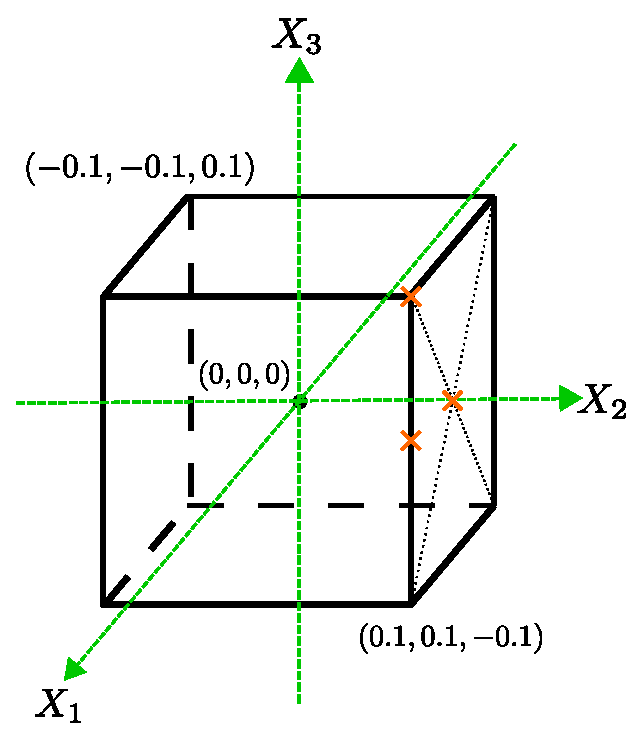
\includegraphics[width=0.35\linewidth]{bild/modul/Asy_plot.eps}%6cm
	\caption{Skizze des Würfels als die Umgebung von der Ruhelage. Die orange Kreuze sind die ausgewählten Anfangspunkte in einer Quadrate.}
	\label{fig:Asy_plot}
\end{figure}

Für dieses Beispiel werden einige Methoden zum Entwurf der Trajektorien von $\vect{u}$ und dann $\vect{x}$ angewendet. Die erste Methode ist noch der Kollokationsverfahren mittels \emph{PyTrajectory}. 

\subsubsection{Trajektorienplanung mit \emph{PyTrajectory}}
Die Einstellung von \emph{PyTrajectory} ist wie folgt: Anfangswerte von freien Parameter $\vect{c}_{f}$ für Spline-Abschnitte sind $0.1$, der Anfangsschätzwert von $k$ ist $1.0$, der Anfangszahl und das Vielfache für den Spline-Abschnitt in der nächsten Iteration ist jeweils $2$.


Mit \emph{PyTrajectory} wird eine Trajektorie von $\vect{u(t)}$ für jeden Ausgangspunkt geplant. Verschiedene Testpunkte benötigen verschiedene Iteration-Mal zwischen $1$ und $3$. Da die Randwerte der Straffunktion sind $k_{min}=0.1$ und $k_{max}=5.0$ gewählt, schwingt der Wert von $k_{end}$ bei unterschiedliche Testpunkte um $2.5$. Abb. \ref{fig:Trajektorien_von_u_1_aus_PyTrajectory} und \ref{fig:Trajektorien_von_u_2_aus_PyTrajectory} zeigen die Simulationskurven der Eingangstrajektorien, die aber keine deutliche Regelmäßigkeit besitzen\footnote{Regelmäßigkeit hier bedeutet, dass die Kurven ca. die gleiche Form besitzen.}\footnote{Zum besser Lesen werden nur fünf Kurven angezeigt. Die gesamten Kurven sind in Abb. \ref{fig:Eingangsverlauf_u1} und \ref{fig:Eingangsverlauf_u2} dargestellt.}. Die Tabelle in dem Anhang \ref{tab:Pytra_Asy_Brockett_Doppelintegrator} beschreibt die Details der Trajektorienkurven. Die Form der Kurven hängt nicht direkt von den Ausgangspunkten ab. In diesem Beispiel werden die Startwerte der Systemzustände gleichzeitig verändert, was die Findung einer Regelmäßigkeit erschwert. Deshalb wird als nächster Schritt die Regelmäßigkeit der Kurven bei der Veränderung nur eines Zustands untersucht.

\begin{figure}[!h]
	\centering
		\includegraphics[width=0.8\linewidth]{bild/30_32/Brockett_e2_Asy_PyTrajectory_d_01_u1.pdf}%12cm
	\caption{Eingangsverläufe $u_{1}$ mit verschiedenen $\vect{x}_{0}$ für Brocketts nicht-holonomen Doppelintegrator mittels \emph{PyTrajectory}.}
	\label{fig:Trajektorien_von_u_1_aus_PyTrajectory}
\end{figure}

\begin{figure}[!h]
	\centering
	\includegraphics[width=0.8\linewidth]{bild/30_32/Brockett_e2_Asy_PyTrajectory_d_01_u2.pdf}%12cm
	\caption{Eingangsverläufe $u_{2}$ mit verschiedenen $\vect{x}_{0}$ für den Brocketts nicht-holonomen Doppelintegrator mittels \emph{PyTrajectory}.}
	\label{fig:Trajektorien_von_u_2_aus_PyTrajectory}
\end{figure}

\textbf{Testpunkte von $x_{1}$ verändert von $-0.1$  bis zu $-0.01$}~~Zuerst wählt man, die Anfangspunkte von $x_{1}$ von $-0.1$ bis zu $-0.01$, mit der Schrittweite $\Delta x_{1} = 0.01$. Die Anfangswerte von $x_{2}$ und $x_{3}$ bleiben in den $10$ Situationen immer $0.1$. 

\begin{figure}[!h]
	\centering
	\begin{subfigure}[c]{\textwidth}
		\centering
		\label{fig:Pytra_x1_-0.09_0.0_deltax=0.01_x_1}
		\includegraphics[width=0.9\linewidth]{bild/30_32/Brockett_e2_local/Pytra_x1_-009_00_deltax=001_x.pdf}
		%\subcaption{Die berechnete Ergebnisse von $\vect{x}$.}	
	\end{subfigure}\\
	%\hspace{-1in} %0.5\textwidth
	\begin{subfigure}[c]{\textwidth}
		\centering
		\label{fig:Pytra_x1_-0.09_0.0_deltax=0.01_x_3}
		\hspace*{-1.7cm}
		\includegraphics[width=0.85\linewidth]{bild/30_32/Brockett_e2_local/Pytra_x1_-009_00_deltax=001_x_3.pdf}
		%\subcaption{Die berechnete Ergebnisse von $u$ und $k$.}
	\end{subfigure}
	\caption{Zustands- und Eingangsverläufe des Doppelintegrator-Systems.}
	\label{fig:Pytra_x1_-0.09_0.0_deltax=0.01_x}
\end{figure}

\begin{figure}[!h]
	\centering
	\includegraphics[width=0.9\linewidth]{bild/30_32/Brockett_e2_local/Pytra_x1_-009_00_deltax=001_u.pdf}%15.5cm
	\caption{Eingangsverläufe mit den Anfangswerten von $x_{1}$ zwischen $-0.10$ und $-0.01$.}
	\label{fig:Pytra_x1_-0.09_0.0_deltax=0.01_u}
\end{figure}

Jeder Fall braucht $2$ oder $3$ Iterationen mit $k_{end}$ zwischen $2.0-2.7$. Wie Abb. \ref{fig:Pytra_x1_-0.09_0.0_deltax=0.01_u} darstellt, geht die Amplitude der ``minus Sinuskurven'' von $u_{1}$ mit der Steigerung von $x_{1,0}$ im Bereich von $(-0.1, -0.03)$ (außer des Falls bei $x_{1,0}=-0.08$) immer herunter, während sich die Amplitude der sinusförmigen Kurve von $u_{2}$ immer vergrößert. Das heißt, in diesem Bereich ergeben sich beide Systemeingänge eine ähnliche Trajektorienform. Über $-0.02$ verkleinert die Amplitude der Kurven sehr schnell zu ungefähr $-1$. (Die Kurven von $-0.02$ und $-0.01$ liegen so nahe, dass nur eine Linie im Bild zu sehen ist. Dieser Effekt tritt z.B. auch bei $x_{3}$ in Abb. \ref{fig:Pytra_x1_-0.09_0.0_deltax=0.01_x} in den Situationen $(-0.08, -0.02,-0.01)$.

Die Zustandverläufe verfügen bei der separaten Veränderung von $x_{2,0}$ und $x_{3,0}$ jeweils in einem kleinen Bereich über auch eine Regelmäßigkeit. Aber wenn die Anfangswerte zwei der drei Systemzustandsvariable gleichzeitig verändert werden, ergeben die Trajektorien keine bestimmte Änderungsregelmäßigkeit. 

Die Trajektorien zeigen eine Regelmäßigkeit in einem kleinen Bereich in dem Brocketts nicht-holonomen System, das die Brockett $2.$ Bedingung nicht erfüllt. Ob diese Regelmäßigkeit auch für das inversen-Pendel-System geeignet ist, lässt sich im nächsten Abschnitt untersuchen. 

\subsection{Eingangsverlauf des inverse-Pendel-Systems}
\label{Ausgang_Das_inverse_Pendel_System}
Die Zustandsfunktion des Benchmark-Systems erfüllt wegen des surjektiven Bildwerts die Brockett $2.$Bedingung. Erinnert man die Gl. \eqref{eq:DLG_Inverses_Pendel_partiell_lin} und lässt sich der Wert von $x_{1}$ von $-1.0$ mit der Schrittweite $h=0.1$ bei jedem Fall zu $-0.4$ vergrößern.

Mit dem Ergebnis in Abb. \ref{fig:Inverses_Pendel_Asy_x1_-10_-04_u} zeigt die Kurven eine ähnliche Regelmäßigkeit wie zuvor: mit Anfangswerte von $x_{1}$ in einem begrenzten Raum ($-1.0,-0.5$) kann man den Linientrend schätzen, außerhalb davon verändert die Kurve mit eine ganz verschiedene Form plötzlich. 
\begin{figure}[!h]
	\centering
	\includegraphics[width=0.95\linewidth]{bild/30_32/Inverses_Pendel_Asy_x1_-10_-04_u.pdf}%15.5cm
	\caption{Eingangsverläufe mit den Anfangswerten von $x_{1}$ zwischen $-1.0$ und $-0.4$.}
	\label{fig:Inverses_Pendel_Asy_x1_-10_-04_u}
\end{figure} 

 In anderen Simulationen, wo $x_{2,0}$ zwischen $(0.2,2.9)$ verändert und $x_{1,0}=x_{4,0}=0, x_{3,0}=\pi$ ist, besitzen alle Trajektorien auch ähnliche Form. Aber die Kombination der obere Untersuchungen, nämlich lässt $x_{1,0}$ und $x_{2,0}$ jeweils in dem Bereich $(-1.0,-0.5)$ und $(0.2,2.9)$ gleichzeitig annehmen, bleiben die Trends alle Kurven nicht identisch (wie Abb. \ref{fig:Inverses_Pendel_Asy_x1_-1_-05_x2-02_30_u}).
\begin{figure}[!h]
	\centering
	\includegraphics[width=0.95\linewidth]{bild/30_32/Inverses_Pendel_Asy_x1_-1_-05_x2-02_30_u.pdf}%15.5cm
	\caption{Eingangsverläufe mit den Anfangswerten von $x_{1}$ zwischen $-1.0$ und $-0.5$ und $x_{2}$ zwischen $0.2$ und $2.9$.}
	\label{fig:Inverses_Pendel_Asy_x1_-1_-05_x2-02_30_u}
\end{figure} 

Daraus ergibt sich die Konsequenz\footnote{Das System des zwei-Gelenken-Manipulators wird auch untersucht, dessen Ergebnis im Anhang \ref{Ausgang_Zwei_Gelenke_Manipulator} gezeigt ist.}: wenn die Anfangswerte von \textbf{nur einem Systemzustandskomponente} in einem \textbf{abgrenzten} Bereich abwandeln, besitzt die Amplitude und die Form der Trajektorienkurven mittels des Python-Pakets \emph{PyTrajectory} eine Regelmäßigkeit. Das gilt in dem System, egal es die Brockett $2.$ Bedingung erfüllt oder nicht. Unter dieser Voraussetzung kann man dann die Möglichkeit eines Steuergesetz $\vect{u(t)}$ überlegen.

\subsection{Entwurf des Steuergesetz mittels Trajektorien aus \emph{PyTrajectory}}
\label{Entwurf_des_Steuergesetz_mittels_Trajektorien_aus_PyTrajectory}
Da die Ueberfuehrungstrajektorien einen allmählich änderte Form in einem Bereich besitzen, ist es möglich, einen Steuergesetz für den gesamten Bereich zu konstruieren. Mit \emph{PyTrajectory} kann im ersten Schritt jeweils eine Trajektorie für die Systemzustandsveränderung aus einigen Startposition in der Umgebung einer Ruhelage in die wie im letzten Abschnitt entworfen werden, dann werden die Trajektorien $\vect{u}_{t}$ mit Interpolation dieser bekannten Trajektorien erstellt.  

Aus Zeitgründen wird in der Arbeit nur ein sehr einfacher Fall vorgestellt: Entwurf des Steuergesetz mit unterschiedlichen $x_{1,0}$.

Wie in dem letzten Abschnitt gezeigt wird, wählt man den Veränderungsbereich von $x_{1,0}$ zwischen $(-0.07,-0.03)$ mit der Schrittweite $0.01$. Die bekannte $\vect{u}(t)$ von \emph{PyTrajectory} mit beispielsweise $p$ Zeitpunkten sind in einer List gespeichert. Die ausgesuchten Eingangstrajektorien mit z.B. $x_{1,0}=-0.043$ braucht zuerst die gehörenden Strecke nämlich einen Bereich zwischen $(-0.05,-0.04)$ zu finden. Damit die Größe der Trajektorie zu jedem Zeitpunkt $p_{i}$ kann mittels der Punkte in der Kurven mit $x_{1,0}=-0.05$ und $-0.04$ linear interpoliert.

Die Interpolationsergebnisse sind in Abb. \ref{fig:Brockett_e2_interpolation_u} und \ref{fig:Brockett_e2_interpolation_x} gezeigt. Nur drei der Trajektorien wurden aus \emph{PyTrajectory} vorgegeben, die anderen sieben sind dadurch interpoliert. In allen Fällen laufen Systemzustandsvariablen schließlich zu der Ruhelage. 
\begin{figure}[!h]
	\centering
	\includegraphics[width=0.8\linewidth]{bild/30_32/Brockett_e2_interpolation_u.pdf}%15.5cm
	\caption{Eingangsverlauf mit dem Anfangszustand von $x_{1}$ in $(-0.05,-0.04)$ mit Interpolation.}
	\label{fig:Brockett_e2_interpolation_u}
\end{figure} 

\begin{figure}[!h]
	\centering
	\includegraphics[width=\linewidth]{bild/30_32/Brockett_e2_interpolation_x.pdf}%15.5cm
	\caption{Zustandsverlauf mit dem Anfangszustand von $x_{1}$ in $(-0.05,-0.04)$ mit Interpolation.}
	\label{fig:Brockett_e2_interpolation_x}
\end{figure} 
 
\section{Trajektorienplanung mit Polynomform von $\vect{u}(t)$}
In diesem Abschnitt wird ein Steuergesetz für das Brockett Beispiel ohne Berücksichtigung der geplannten Trajketorien aus \emph{Pytrajectory} diskutiert. Zuerst wird eine Polynomform für die Systemeingänge aufgestellt, die die $2$. Bedingung von Brockett erfüllt.

Es wird angenommen, dass $u_{1}$ und $u_{2}$ jeweils ein Polynom der Zeit $t$ ist:
\begin{eqnarray}
u_{1} &=& a_{0}+a_{1}t+a_{2}t^{2}\notag\\
u_{2} &=& b_{0}+b_{1}t+b_{2}t^{2}.
\label{eq:Brocketts_Beispiel_u}
\end{eqnarray}
Integriert man die ersten zwei Gleichungen in Gl. \eqref{eq:Brocketts_Beispiel_u}, erhält man:
\begin{eqnarray}
x_{1} &=& a_{0}t +\frac{1}{2}a_{1}t^{2}+\frac{1}{3}a_{2}t^{3}+\alpha \notag\\
x_{2} &=& b_{0}t +\frac{1}{2}b_{1}t^{2}+\frac{1}{3}b_{2}t^{3}+\beta.
\label{eq:Brocketts_Beispiel_x1_x2}
\end{eqnarray}
Setzt man Gln. \eqref{eq:Brocketts_Beispiel_u}, \eqref{eq:Brocketts_Beispiel_x1_x2} in die letzte Zeile von Gl. \eqref{eq:Brockett_Doppelintegrator_ch4} ein\footnote{Der Koeffizient von $t^{5}$ ist gleich null.}:
\begin{eqnarray}
\dot{x}_{3} &=& x_{2}u_{1}-x_{1}u_{2} = (a_{0}\beta-b_{0}\alpha) + t(a_{1}\beta-b_{1}\alpha)\notag\\ &+& t^2(\frac{1}{2}a_{1}b_{0}-\frac{1}{2}a_{0}b_{1}+a_{2}\beta-b_{2}\alpha)+\frac{2}{3}t^3(a_{2}b_{0}-a_{0}b_{2})+\frac{1}{6}t^4(a_{2}b_{1}-a_{1}b_{2})
\label{eq:Brocketts_Beispiel_dot_x3}
\end{eqnarray}
daraus folgt die Form von $x_{3}$:
\begin{eqnarray}
{x}_{3} &=& t(a_{0}\beta-b_{0}\alpha) + \frac{1}{2}t^{2}(a_{1}\beta-b_{1}\alpha)\notag\\ &+& \frac{1}{3}t^3(\frac{1}{2}a_{1}b_{0}+\beta a_{2}-\frac{1}{2}a_{0}b_{1}-\alpha b_{2})+\frac{1}{6}t^4(a_{2}b_{0}-a_{0}b_{2})+\frac{1}{30}t^5(a_{2}b_{1}-a_{1}b_{2}) + \gamma\notag\\
\label{eq:Brocketts_Beispiel_x3}
\end{eqnarray}

Falls die gesamte Überführungszeit $T=1s$ ist, dann :
\begin{eqnarray}
x_{1,end} &=& a_{0}+\frac{1}{2}a_{1}+\frac{1}{3}a_{2} + \alpha\stackrel{!}{=}0\notag\\
x_{2,end} &=& b_{0}+\frac{1}{2}b_{1}+\frac{1}{3}b_{2} + \beta\stackrel{!}{=}0\notag\\
{x}_{3,end} &=& (a_{0}\beta-b_{0}\alpha) + \frac{1}{2}(a_{1}\beta-b_{1}\alpha)\notag\\ &+& \frac{1}{3}(\frac{1}{2}a_{1}b_{0}+\beta a_{2}-\frac{1}{2}a_{0}b_{1}-\alpha b_{2})+\frac{1}{6}(a_{2}b_{0}-a_{0}b_{2})+\frac{1}{30}(a_{2}b_{1}-a_{1}b_{2}) + \gamma\stackrel{!}{=}0\notag\\
\label{eq:Brocketts_Beispiel_t_1s}
\end{eqnarray}


Gl. \eqref{eq:Brocketts_Beispiel_t_1s} ist ein unterbestimmtes Gleichungssystem mit $6$ Variablen und $3$ Funktionen. Als Beispiel wählt man hier $a_{0}$, $a_{1}$ und $b_{0}$ als unabhängige Variablen, dann lassen sich $a_{0}$, $b_{1}$ und $b_{2}$ daraus darstellen:
\begin{eqnarray}
a_{2} &=& - 3.0 a_{0} - 1.5 a_{1} - 3.0 \alpha\notag\\
b_{1} &=& \frac{1}{a_{0} + 6.0 \alpha} \left(30.0 a_{0} \beta + a_{1} b_{0} + 6.0 a_{1} \beta - 30.0 \alpha b_{0} + 60.0 \gamma\right)\notag\\
b_{2} &=& \frac{1}{a_{0} + 6.0 \alpha} \left(- 3.0 a_{0} b_{0} - 48.0 a_{0} \beta - 1.5 a_{1} b_{0} - 9.0 a_{1} \beta + 27.0 \alpha b_{0} - 18.0 \alpha \beta - 90.0 \gamma\right)\notag\\
\label{eq:Brockett_e2_u(t)_polynom_a2_b1_b2}
\end{eqnarray}
Zur Vermeidung der Singularität muss $a_{0}\neq -6\alpha$ sein. Unter dieser Beschränkung können $\alpha,\beta,\gamma$ und $a_{0}, a_{1}, b_{0}$ beliebig gewählt werden. (Daher ist der Ursprung mit dem polynomischen Steuergesetz $\vect{u}(t)$ asymptotisch stabil.)

Das heißt, diese Form von $\vect{u}(t)$ ermöglicht es, eine Trajektorie von $\vect{x}(t)$ von irgend einem Punkt in einer Umgebung der Ruhelage in die Ruhelage führen zu lassen. Zur Verifizierung verwendet man hier auch den Würfel mit der Seitenlänge $0.1$ als die Umgebung und die $27$ Testpunkte als Anfangswerte von $\vect{x}$. Die anderen Parameter sind wie so eingestellt: $a_{0}=a_{1}=b_{0}=1$.

Die berechnete Kurven stehen in Abb. \ref{fig:Brockett_e2_Asy_u(t)_dx_01_x} und \ref{fig:Brockett_e2_Asy_u(t)_dx_01_u}. Wie erwartet läuft die Trajektorie von $\vect{x}$ in jedem Fall von der bestimmten Ausgangspunkt zur Ruhelage. Ein interessantes Phänomen liegt in den Abbildungen von $x_{1}$ und $u_{1}$: es gibt nur $3$ Kurven in jedem Bild. Die Erklärung dafür ist mit den Definitionsgleichungen Gl. \eqref{eq:Brocketts_Beispiel_u} und \eqref{eq:Brocketts_Beispiel_x1_x2} einfach: $u_{1}$ und $x_{1}$ sind nur von $a_{0}$, $a_{1}$ und $a_{2}$ abhängig, wobei der ersten zwei konstant $1$ sind und $a_{2} =-3a_{0}-1.5a_{1}-3\alpha$ mit $\alpha$ zu $(-0.1,0.0,0.1)$ gehört (Fall $1-9:\alpha=-0.1$, Fall $10-18:\alpha=0.0$ und Fall $19-27:\alpha=0.1$). 
\begin{figure}[!h]
	\centering
	\includegraphics[width=\linewidth]{bild/30_32/Brockett_e2_Asy_u(t)_dx_01_x.pdf}%15.5cm
	\caption{Verlauf der Zustandskomponente mittels Polynom-Ansatz für $\vect{u}$.}
	\label{fig:Brockett_e2_Asy_u(t)_dx_01_x}
\end{figure}

\begin{figure}[!h]
	\centering
	\includegraphics[width=0.8\linewidth]{bild/30_32/Brockett_e2_Asy_u(t)_dx_01_u_old.pdf}%13cm
	\caption{Verlauf der Systemeingänge mittels Polynom-Ansatz für $\vect{u}$.}
	\label{fig:Brockett_e2_Asy_u(t)_dx_01_u}
\end{figure}

Die Form von $\vect{u}$ ist zwar relativ einfach, aber zum Zeitpunkt $t=0s$ und $t=1s$ hat $u_{1}$ einen Sprung von $0$ zu $1$ und von $-2.5$ zu $0.0$, und zu $t=1s$ verschwindet $u_{2}$ die Stetigkeit auch. In dem nächsten Abschnitt werden zwei Regelgesetze entworfen.

\section{Reglerentwurf für den Brocketts nicht-holonomen Doppelintegrator in \cite{liberzon2012switching}}
\label{Reglerentwurf_für_den_Brocketts_nichtholonomischen_Doppelintegrator_in_Literatur_liberzon2012switching}
Aus Abschnitt \ref{Erläuterung_zur_Brockett-Bedingung} ist schon bekannt, der Brocketts nichtholonomer Doppelintegratordie Brocketts Bedingung nicht erfüllt, deshalb existiert kein $C^{1}$ Regelgesetz, dass die Ruhelage dieses Systems asymptotisch stabilisiert wird. In der Literatur \cite{liberzon2012switching} stellte der Autor D. Liberzon einen Schaltregelgesetz auf, mit dem die Systemzustände aus einem Punkt in der Umgebung der Ruhelage endlich zur Ruhelage gehen können.

Ausgangspunkt ist die Transformation der Systemdarstellung in Kartesischen Koordinaten zur Zylinderkoordinaten. Anhand der Umrechnung:
\begin{eqnarray}
r &=& \sqrt{x_{1}^{2}+x_{2}^{2}}\notag\\
\varphi &=& \mathrm{arctan2}(x_{2},x_{1})\notag\\
z &=& x_{3}
\label{eq:Darsgellung_von_Kar_und_Zylinder}
\end{eqnarray}
und 
\begin{eqnarray}
u_{z} &=& \cos(\varphi)u_{1} + \sin(\varphi)u_{2}\notag\\
v_{z} &=& \cos(\varphi)u_{2} - \sin(\varphi)u_{1}
\end{eqnarray} 
erhält man die Systemgleichungen in Zylinderkoordinaten:
\begin{eqnarray}
	\dot{r} &=& u_{z}\notag\\
	\dot{\varphi} &=& \frac{v_{z}}{r}\notag\\
	\dot{z} &=& -r\cdot v_{z}.
	\label{eq:Brockett_e2_in_Zylinderkoordinaten}
\end{eqnarray}  
In \cite{liberzon2012switching} wird das Regelgesetz: 
\begin{eqnarray}
	u_{z} &=& -r^2\notag\\
	v_{z} &=& z
	\label{eq:Brockett_e2_Switch_Regelgesetz}
\end{eqnarray}
entworfen. Der Regler ist geeignet für alle Anfangspunkte außerhalb der Situation bei\footnote{Die Erklärung kann man in der Literatur \cite{liberzon2012switching} lesen.} $r_{0}=0$, deswegen muss man bei $r_{0}$ einen neuen Regler anwenden, um die Trajektorie die z-Achse zu verlassen. Ein möglicher Regler lässt sich wie z.B. $u_{z}=1, v_{z}=0$ in einem begrenzten Anfangszeit $T_{phase1}$ entwerfen, damit $r$ genug weit von $z$-Achse geht während $\varphi$ und $z$ still bleiben. Bemerkenswert ist, dass der Wert von $r$ immer größer gleich wie $0$ ist. Nach der Zeit $T_{phase1}$ funktioniert wieder das Regelgesetz aus Gl. \eqref{eq:Brockett_e2_Switch_Regelgesetz}.

Zwei Fälle werden für die Idee auf das System getestet. Zunächst fängt man mit der Trajektorieplanung mit dem Anfangszustand gleich $(0,5,5)$ an. $T_{phase1}$ ist als $0.2s$ eingestellt. Die Linie von $r$ in Abb. \ref{fig:Brockett_e2_Switch_ein_Fall} nimmt in den ersten $0.2s$ zu ungefähr $0.2$ zu, danach fällt sie bis zur Endzeit $T_{end}$ langsam ab. Innerhalb von $0.2s$ bleiben die Werte von $\varphi$ und $z$ unverändert, dann nehmen beide zu. Es ist zu beachten, dass $r$ und $z$ zu $0$ konvergieren können, aber die Tendenz von $\varphi$ neigt nicht zu $0$ (aber mit einem großen oder kleinen $\varphi_{end}$ kann das Systemzustandsvektor noch in die Ruhelage erreichen, sobald der Radius $r$ und die Höhe $z$ gleich null sind.). Abb. \ref{fig:3d_Brockett_e2_Switch} zeigt die dreidimensionale Trajektorie mit zwei Phasen deutlich.
\begin{figure}[!h]
	\centering
	\includegraphics[width=\linewidth]{bild/30_32/Brockett_e2_Switch_x.pdf}%13cm
	\caption{Zustandsverläufe in Zylinderkoordinaten mit dem Startwert $(0,5,5)$.}
	\label{fig:Brockett_e2_Switch_ein_Fall}
\end{figure}

\begin{figure}[!h]
	\centering
	\includegraphics[width=0.8\linewidth]{bild/30_32/3d_Brockett_e2_Switch.pdf}%13cm
	\caption{3D-Kurve von Systemzustand in Zylinderkoordinaten mit dem Startwert $(0,5,5)$.}
	\label{fig:3d_Brockett_e2_Switch}
\end{figure}


\begin{figure}[!h]
	\centering
	\includegraphics[width=\linewidth]{bild/30_32/Brockett_e2_Switch.pdf}%15.5cm
	\caption{Trajektorien von $r,\varphi,z$ mit unterschiedlichen Anfangswerten.}
	\label{fig:Brockett_e2_Switch}
\end{figure}

In der zweiten Situation stellt man unterschiedliche zufällige Anfangswerte von Zustände innerhalb von $[-0.5,0.5)$ ein\footnote{Bei dem Fall $r<0$ wird $r$ durch der absolute Betrag ersetzt.}. Wie in Abb. \ref{fig:Brockett_e2_Switch} zu sehen ist, konvergieren $r$ und $z$ zu $0$ mit einer kleinen Geschwindigkeit, während die Kurven von $\varphi$ in den meisten Fällen divergieren.

Zusammengefasst funktioniert das Regelgesetz, aber mit dem Schönheitsfehler einer langsamen Konvergenzgeschwindigkeit. Zur Verbesserung wird ein komplexeres Regelgesetz im nächsten Abschnitt vorgestellt.

\section{Ein dreiphasiger Reglerentwurf für Brocketts nichtholonomen Doppelintegrator}
\label{Ein_dreiphasiger_Reglerentwurf_für_den_Brocketts_nichtholonomischen_ Doppelintegrator}
In Zusammenarbeit mit dem Betreuer dieser Arbeit werde der folgende Ansatz entwickelt: ein schaltendes Regelgesetz mit zwei oder drei Phasen ist geeignet, um die Trajektorien aller Systemzustände in $(0,0,0)$  erfolgreich anzukommen. Der Gedankengang kommt aus der Analyse der Trajektorie des Zustandsvektors. Ähnlich wie Gl. \eqref{eq:Darsgellung_von_Kar_und_Zylinder} im letzten Abschnitt kann die Zustandsfunktion mit der Definition von Systemeingänge in die Zylinderkoordinaten transformiert werden:
\begin{eqnarray}
\dot{r} &=& \cos(\varphi)u_{1} + \sin(\varphi)u_{2} =:u_{z}\notag\\
\dot{\varphi} &=& \frac{1}{r}(u_{2}\cos(\varphi)-u_{1}\sin(\varphi)) =: v_{z}\notag\\
\dot{z} &=& r(sin(\varphi)u_{1}-\cos(\varphi)u_{2})= -v_{z}r^{2}.
\label{eq:Ableitung_r_phi_z_in_Zylinderachse}
\end{eqnarray}

Unter einer Schraubenlinie versteht man eine Kurve, die mit dem unveränderten Radius nach unten/oben rotiert. Auf der Basis kann eine Trajektorie von Systemzustand mit irgend einem Startwert weit von $z$-Achse ähnlich wie eine Schraubenlinie in die $z=0$ Ebene gehen. Die Skizze ist in Abb. \ref{fig:Schraubenlinie} zu sehen.
\begin{figure}[!h]
	\centering
	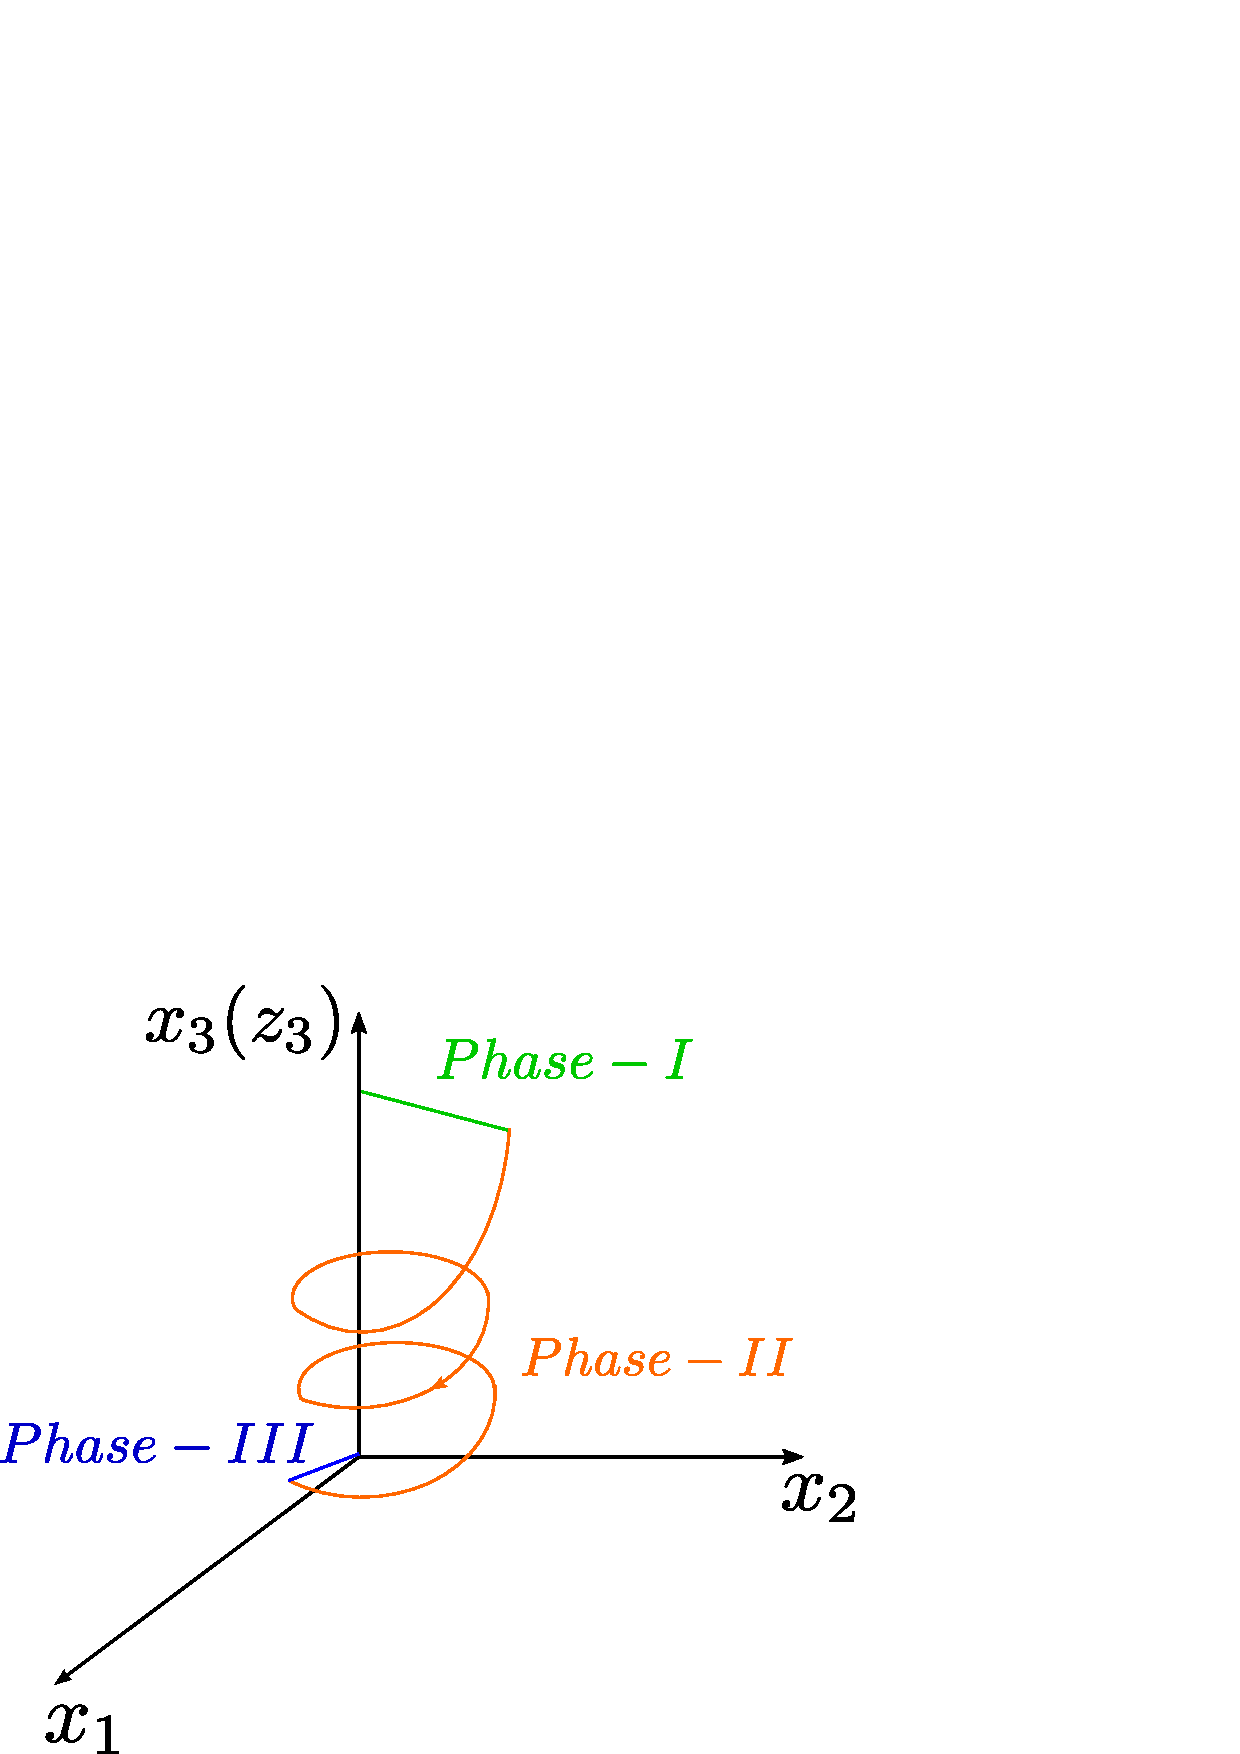
\includegraphics[width=0.4\linewidth]{bild/modul/Schraubenlinie.pdf}%12cm
	\caption{Skizze der Trajektorie des Zustandsvektors mit der Schraubenlinie.}
	\label{fig:Schraubenlinie}
\end{figure}

Wenn $r>0$ läuft die Trajektorie von $\vect{x}$ in Phase-II von $x_{3,0}$ bis zur $X_{1}$-$X_{2}$-Ebene bei $x_{3,0}>0$ abwärts, sonst von unten nach oben. Wenn der Punkt auf der $X_{1}$-$X_{2}$-Ebene weit von der Ruhelage liegt, kann sich der Regler in Phase-III so einstellen lassen, dass $x_{1}$ und $x_{2}$ (oder $r$ in der Zylinderkoordinate) nach und nach bis zu $0$ verkleinern und gleichzeitig $x_{3}$ (oder $z$ in Zylinderkoordinate) noch $0$ bleibt. 

Ein Ausnahme steht in der Situation, wenn der Anfangswert von $\vect{x}$ auf der $z$-Achse liegt. Bei $x_{1,0}$ und $x_{2,0}$ beide $0$ ist der Radius $r_{0}$ auch $0$. Unter der Berücksichtigung der Unveränderlichkeit von $r$ in der ganzen Phase-II ändert sich $\dot{z}$ in Gl. \eqref{eq:Ableitung_r_phi_z_in_Zylinderachse} auch nicht. Deswegen kann die Trajektorie nie nur mittels der vorherigen Idee zur Ruhelage erreichen. Dieses Problem kann man mit dem Entwurf einer zusätzlichen Phase vor Phase-II gelöst werden. Während der Phase-I verändert nur $r$, der am Ende dieser Phase weit von der $z$-Achse liegt.

Und schließlich ergibt sich noch eine Frage: Wie weit muss sich $r$ in Phase-I von $z$-Achse entfernen? Das Problem kann man mit dem kürzesten Weg der gesamten Trajektorie beantworten. Die Länge des Pfads der drei Pahsen ist\footnote{Der detaillierte Rechenverlauf ist in Anhang \ref{Rechenverlauf_fuer_L_Tra} dargestellt}: 
\begin{eqnarray}
L_{Tra} &=& r_1 + \int_{0}^{T_{2}} \sqrt{\dot x_1^2 + \dot x_2^2 + \dot x_3^2 }\, dt + r_1 \notag\\&=& \frac{z_{0}}{r_{1}}\sqrt{r_{1}^{2}+1} + 2r_{1}
\label{eq:Länge_der_Schraubenkurve}
\end{eqnarray} 
wobei die Bogenlänge in Phase-I gleich ist wie in Phase-III und mit $r_{1}$ gekennzeichnet wird. $T_{2}$ steht für die Überführungszeit in Phase-II. Setzt man die Ableitung von $L_{Tra}$ nach $r_{1}$:
\begin{eqnarray}
\frac{\partial L_{Tra}}{\partial r_{1}} = \frac{z_{0}}{\sqrt{r_{1}^{2} + 1}} - \frac{z_{0}}{r_{1}^{2}} \sqrt{r_{1}^{2} + 1} + 2
\label{eq:Ableitung_von_L_Tra}
\end{eqnarray} 
gleich null ein, wird eine von $z_{0}$ abhängigen optimale Bogenlänge in Phase-I $r_{1,opt}$ ausgerechnet, mit der $L_{Tra}$ am kleinsten ist. Wenn der Anfangswert von $r_{0}$ kleiner als $r_{1,opt}$ ist, soll $r$ noch weiter von $z$ entfernen. Im anderen Fall geht das System mit dem Regelgesetz direkt in die Phase-II.

Der nächste Schritt ist der Entwurf von $\vect{u}$ gemäß der obere Idee. Fängt man mit dem Systemeingang in Phase-I an. Wie gerade diskutiert soll nur $r$ innerhalb von diesen Phase verändern werden, dann lässt sich $u_{z}=1$ und $v_{z}=0$ einsetzen. In Phase-II ist es gerade umgekehrt, $u_{z}=0$ und $v_{z}=sign(z)$, sodass der Absolutwert von $z$ immer kleiner wird. Am Ende wenn die Trajektorie schon auf $X_{1}$-$X_{2}$-Ebene sehr nähe liegt, wird der Radius $r$ mit $u_{z}=-1$ und $v_{z}=0$ verkleinert. 

\begin{figure}[!h]
	\centering
	\includegraphics[width=\linewidth]{bild/30_32/Brockett_e2_ck_x.pdf}%13cm
	\caption{Zustandsverläufe mit dem Startwert $(0,5,5)$.}
	\label{fig:Brockett_e2_ck_ein_Fall}
\end{figure}

Dieses Regelgesetz wird auch wieder in zwei Fällen getestet. Der erste ist ähnlich wie dem letzten Abschnitt in Bezug auf \emph{einen} Startwert von $\vect{x}$. Abb. \ref{fig:Brockett_e2_ck_ein_Fall} und \ref{fig:3d_Brockett_e2_ck} zeigen die simulierten Ergebnissen mit $\vect{x}_{0}=(0,0,5)$ und $T_{end}=6s$. Die Ergebnisse entsprechen der Erwartung. $r_{1,opt}$ ist ungefähr $1.29$. Mit $u_{z}/v_{z}=1$ dauern die Phase-I und Phase-III jeweils $1.29s$.
\begin{figure}[!h]
	\centering
	\includegraphics[width=0.8\linewidth]{bild/30_32/3d_Brockett_e2_ck.pdf}%13cm
	\caption{3D-Kurve des Systemzustands mit dem Startwert $(0,5,5)$.}
	\label{fig:3d_Brockett_e2_ck}
\end{figure}

Das zweite Beispiel zielt auf die Prüfung der asymptotischen Stabilität der Ruhelage $(0,0,0)$. Anfangswerte sind eine zufällige Liste mit $20$ Elementen, die in dem Wertebereich $[-0.5,0.5)$ liegen. Der Endzeit $T_{end}=4s$. Als Ergebnis kann die Trajektorie in jedem Fall die Ruhelage erreichen. Die asymptotische Stabilität wird dadurch verifiziert.

\begin{figure}[!h]
	\centering
	\includegraphics[width=\linewidth]{bild/30_32/Brockett_e2_ck_x_Asy.pdf}%13cm
	\caption{Zustandsverläufe mit unterschiedlichen Anfangswerten.}
	\label{fig:Brockett_e2_ck_x_Asy}
\end{figure}

Im Vergleich mit dem Regelgesetz aus Literatur \cite{liberzon2012switching} b.z.w. Abschnitt \ref{Reglerentwurf_für_den_Brocketts_nichtholonomischen_Doppelintegrator_in_Literatur_liberzon2012switching} hat dieses einige Vorteile. Ein wichtiger Punkt liegt in die kürze Konvergenz-Zeit der Trajektorie. Mit gleichen Anfangswerten von $\vect{x}_{0}$ ist die Trajektorie mit dem Regelgesetz in \cite{liberzon2012switching} in $10s$ noch nicht fertig, während die mit diesem Regelgesetz nach $3s$ schon zur Ruhelage ankommt. Die Konvergenzgeschwindigkeit ist deutlich schneller.

Bemerkenswert ist, dass das in drei Phasen schaltende Regelgesetz nicht kontinuierlich ist, nämlich die Brockett Bedingung nicht verletzt. 

Fazit: In diesem Kapitel wurden einige Steuerung und Regler für die Untersuchung der asymptotischen Stabilität der Ruhelage in Brocketts berühmten nicht-holonomen Doppelintegrator vorgestellt. Jeder kann die Trajektorie schließlich in die Ruhelage führen, auch wenn jeder nicht stetig differenzierbar ist. Das steht im Einklang mit Brocketts Bedingungen.
\chapter{Zusammenfassung und Ausblick}
\label{ch:Zusammenfassung_und_Ausblick}
\section{Zusammenfassung}
Das Ziel der vorliegenden Diplomarbeit war die Analyse der Überführungstrajektorien eines unteraktuierten Systems aus der Umgebung einer Ruhelage in diese Ruhelage mittels des Python-Pakets \emph{PyTrajectory}, welches um eine Funktion der Bestimmung der optimalen Überführungszeit erweitert wurde. 

Das Theorem von Brockett zur Bestimmung der Existenz einer stetigen differenzierbaren Regelgesetz wurde zuerst in Kapitel \ref{ch:Brockett_Bedingung_für_unteraktuiertes_mechanisches_System} vorgestellt. Als Anwendung existiert für das in Kapitel \ref{ch:Trajektorieplanung_durch_Lösung_einer_Randwertaufgabe} und \ref{ch:Reglerentwurf-durch-Trajektorieplanung} betrachtete Beispiel-das nicht-holonomen Doppelintegrator-System nach Brocketts Theorem keines stetig differenzierbares Regelgesetz zu verfügen, um die Ruhelage asymptotisch zu stabilisieren. Im Gegensatz dazu erfüllt das berühmte Benchmark System-``inverse-Pendel'' diese notwendige Bedingung.

Zum Vergleich der Überführungstrajektorien dieser zwei Systeme wurde das Python-Paket \emph{PyTrajectory} als das Werkzeug verwendet, um die Trajektorien durch Lösung einer Randwertaufgabe zu entwerfen. Eine Funktion davon wurde erweitert, damit die Überführungszeit des Regelvorgangs auch ein Berechnungsergebnis ist, statt vom Nutzer vorgegeben zu werden. Der Ausgangspunkt lag in der Transformation der Zeitkoordinaten, die durch die Ergänzung eines zusätzlichen Parameters in der Systemzustandsfunktion realisiert wurde. Aber wegen des nicht brauchbaren Ergebnis des Parameters wurde eine Straffunktion entworfen, mit der eine bessere Lösung ausgerechnet wurde.

Danach wurde die Überführugstrajektorie zweier Systeme mit unterschiedlichen Anfangswerten von Systemzuständen mittels \emph{PyTrajectory} analysiert. Die Regelmäßigkeit der Trajektorien ist nur in einem \textbf{begrenzten} Bereich für beide Systeme effektiv hängt nicht davon, ob das System die Brockett-Bedingung bezüglich erfüllt. Mit anderen Worten ist die Konstruktion eines Regelgesetz zur Lösung der Randwertaufgabe mit Anfangszuständen in einer relativ großen Umgebung der Ruhelage schwierig. Aus diesem Grund wurden in Kapitel \ref{ch:Reglerentwurf-durch-Trajektorieplanung} einige nicht stetig-differenzierbaren Regelgesetze unter Berücksichtigung der Besonderheit der Systemzustandsdarstellung für den nicht-holonomen Doppelintegrator entworfen, mit den die Trajektorien aus der Umgebung der Ruhelage in diese ermöglicht wurden. 
\section{Ausblick}
\label{Ausblick}
Für die Zukunft empfiehlt die Autorin die Vervollständigung der Analyse der Überführungstrajektorien aus einer Umgebung der gewünschten Ruhelage in diese. In der Arbeit wurden nur drei typischen unteraktuierte Systeme untersucht. Das Modell wie das Acrobot-System \cite{spong1995swing} wäre beispielsweise ein guter Anfangspunkt.

Aus Zeitgründen erwägt die Autorin in der Arbeit den Entwurf eines Steuergesetzes durch die Interpolation der ausgerechneten Trajektorien aus $\emph{PyTrajectory}$, das nur in einem sehr einfachen Fall verwendet wurde, wobei sich nur ein Systemzustandselement in einem Bereich veränderte. Die Konstruktion eines Regelgesetz zur Lösung der Randwertaufgabe mit den Anfangswerten von $\vect{x}$ in zweidimensionalen Umgebung der Ruhelage soll auch durch Interpolation bekannter Trajektorien umsetzbarmöglichst geringer Bogenlängemöglichst geringer Bogenlänge sein. 

%*******************************************************************************
% * Copyright (c) 2006-2013 
% * Institute of Automation, Dresden University of Technology
% * 
% * All rights reserved. This program and the accompanying materials
% * are made available under the terms of the Eclipse Public License v1.0 
% * which accompanies this distribution, and is available at
% * http://www.eclipse.org/legal/epl-v10.html
% * 
% * Contributors:
% *   Institute of Automation - TU Dresden, Germany 
% *      - initial API and implementation
% ******************************************************************************/
\begin{appendices}
	\chapter{Appendix}
	\label{sec:Appendix}
	
	%%%%%%%%%%%%%%%%%%%%%%%%%%%%%%%%%%%%%%%%%%%%%%%%%%%%%%%%%%%%%%%%%%%%%%
	\section{Zwei-Gelenke-Manipulator}
	\label{Ausgang_Zwei_Gelenke_Manipulator}
	Das zwei-Gelenke-Manipulator besteht aus vier Zustandskomponente mit der Systemzustandsgleichung \cite{CK}:
	\begin{eqnarray}
		\dot{x}_{1} &=& x_{2}\notag\\
		\dot{x}_{2} &=& u_{1}\notag\\
		\dot{x}_{3} &=& x_{4}\notag\\
		\dot{x}_{4} &=& -\eta x_{2}^2\cdot \sin(x_{3})-(1+\eta \cos(x_{3}))\cdot u_{1}.
		\label{eq:Zwei-Gelenke-Manipulator}
	\end{eqnarray}
	In Abb. \ref{fig:Zwei_Gelenke_Mainipulator} ist $x_{1}$ und $x_{2}$ jeweils der Winkel und Winkelgeschwindigkeit des ersten Gelenks und $x_{3}$ und $x_{4}$ des zweiten Gelenks. $\eta = \frac{m_{2}l_{1}r_{2}}{J_{2}+m_{2}r_{2}^{2}}$ ist der Trägheitsparameter.
	\begin{figure}[!h]
		\centering
		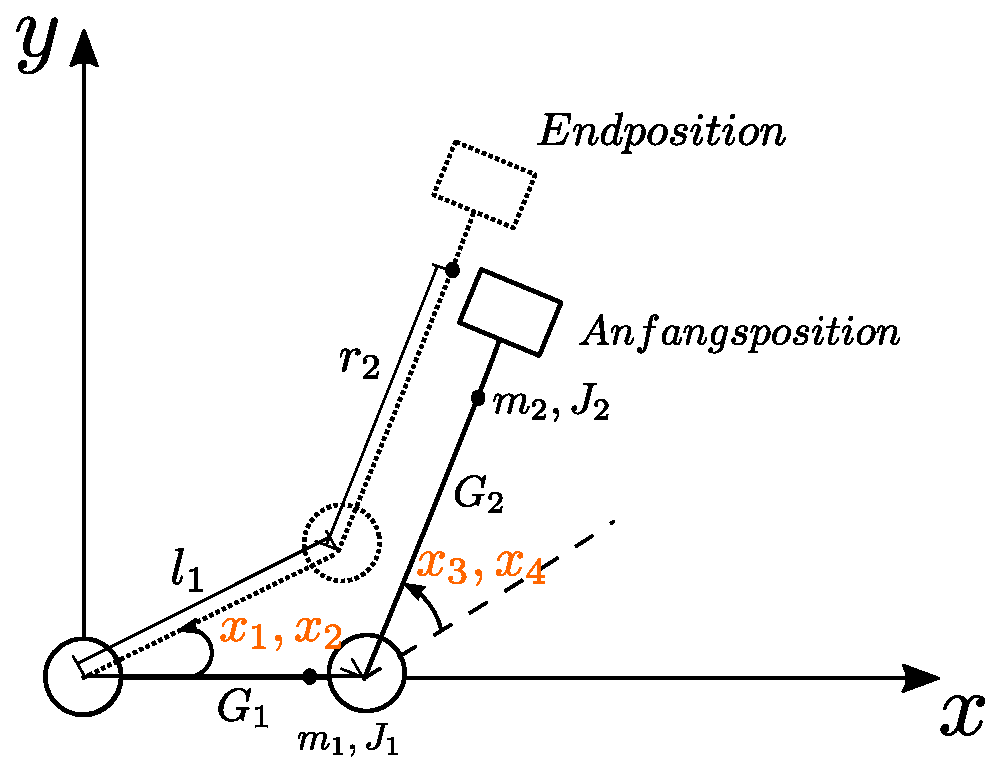
\includegraphics[width=0.5\linewidth]{bild/modul/Unteraktuiertes-System.eps}
		\caption{Skizze eines Zwei-Gelenke-Manipulators.}
		\label{fig:Zwei_Gelenke_Mainipulator}
	\end{figure}
	Der Manipulator erfüllt die Brockett $3.$ Bedingung nicht (mit dem Bild $(0,0,0,\varepsilon)^{T}$).
	
	Für die Simulation in Abschnitt \ref{Einfluss_der_Startschätzung_von_cf} sollte der Manipulator sich von $(0,0,72^{\circ},0)$ zu $(36^{\circ},0,36^{\circ},0)$ bewegen. Die Randwerte von $k$ sind wie $0.1$ und $15$ eingestellt. Anfangssplineabschnitte von $\vect{x}$ und $\vect{u}$ sind $10$ und $20$.
	
	Für die Simulation in Abschnitt \ref{Ausgang_Das_inverse_Pendel_System} ist die Umgebung von $\vect{x}_{3,0}$ zuerst eine Strecke von $63^{\circ}$ zu $81^{\circ}$. Abb. \ref{fig:example4_x3_035pi_045pi_u} zeigt, nur im Bereich von $(63^{\circ}-73.8^{\circ})$ verändert die Form der Trajektorien regelmäßig.
	\begin{figure}[!h]
		\centering
		\includegraphics[width=\linewidth]{bild/30_32/example4_x3_035pi_045pi_u.pdf}
		\caption{Trajektorien des Systemeingangs mit unterschiedlichen Anfangswerten von $x_{3}$}
		\label{fig:example4_x3_035pi_045pi_u}
	\end{figure}
	Die Trajektorien bei der Veränderung von $x_{1,0}$ im Bereich $(-9^{\circ}-9^{\circ})$ ist in Abb. \ref{fig:example4_x1_-005pi_005pi_u} dargestellt. Ähnlich wie Ergebnis von der Veränderung von $x_{3}$ ist die Form von $u_{t}$ zwischen $-9^{\circ}$ und $1.8^{\circ}$ regelmäßig. 
	\begin{figure}[!h]
		\centering
		\includegraphics[width=\linewidth]{bild/30_32/example4_x1_-005pi_005pi_u.pdf}
		\caption{Trajektorien des Systemeingangs mit unterschiedlichen Anfangswerten von $x_{1}$.}
		\label{fig:example4_x1_-005pi_005pi_u}
	\end{figure}
	Lässt sich $x_{1,0}$ und $x_{3,0}$ gleichzeitig verändern jeweils im Raum von $(-9^{\circ}-1.8^{\circ})$ und $(63^{\circ}-73.8^{\circ})$ ergibt sich für alle Trajektorien keine ähnliche Form. (Der regelmäßige Bereich ist weiterhin begrenzt.)
	\begin{figure}[!h]
		\centering
		\includegraphics[width=\linewidth]{bild/30_32/example4_x1_-005pi_001pi_x3_035pi_041pi_u.pdf}
		\caption{Trajektorien des Systemeingangs mit unterschiedlichen Anfangswerten von $x_{1}$ und $x_{3}$.}
		\label{fig:example4_x1_-005pi_001pi_x3_035pi_041pi_u}
	\end{figure}
	\clearpage
	\section{Tabelle für die Überprüfung der asymptotischen Stabilität des Brocketts nicht-holonomen Doppelintegrators}
	\label{sec:Tabelle_Brockett_e2}
	%%%%%%%%%%%%%%%%%%%%%%%%%%%%%%%%%%%%%%%%%%%%%%%%%%%%%%%%%%%%%%%%%%%%%%
	
	\begin{table}[htbp]
		\centering
		\caption{Die Form der Trajektorienkurve des Systemeingangs $u_{1}$ mit unterschiedlichen Anfangswerte von $\vect{x}$}
		\label{tab:Pytra_Asy_Brockett_Doppelintegrator}
		\begin{tabular}{{p{5.3cm}p{5cm}}}
			Testpunkte $(x_{1,0},x_{2,0},x_{3,0})$ & Form der Kurve\\
			\toprule
			$(-1,0,0)$ & sinusförmig\\
			$(-1,1,0)$ & sinusförmig\\
			$(0,-1,0)$ & sinusförmig\\
			$(0,-1,1)$ & sinusförmig\\
			$(0,0,-1)$ & sinusförmig\\
			$(0,1,-1)$ & sinusförmig\\
			$(1,-1,-1)$ & sinusförmig\\
			$(1,-1,1)$ & sinusförmig\\
			$(1,0,-1)$ & sinusförmig\\
			$(1,1,-1)$ & sinusförmig\\
			$(1,1,1)$ & sinusförmig\\
			$(1,1,0)$ & parabelförmig\\
			$(-1,-1,-1)$ & kosinusförmig\\
			$(-1,-1,0)$ & kosinusförmig\\
			$(-1,-1,1)$ & kosinusförmig\\
			$(-1,0,-1)$ & kosinusförmig\\
			$(-1,0,1)$ & kosinusförmig\\
			$(-1,1,-1)$ & kosinusförmig\\
			$(-1,1,0)$ & kosinusförmig\\
			$(0,-1,-1)$ & kosinusförmig\\
			$(0,0,0)$ & kosinusförmig (Ruhelage)\\
			$(0,1,0)$ & kosinusförmig\\
			$(0,1,1)$ & kosinusförmig\\
			$(1,-1,0)$ & kosinusförmig\\
			$(1,0,0)$ & kosinusförmig\\
			$(1,0,1)$ & kosinusförmig\\
			$(1,1,0)$ & kosinusförmig\\	
			\bottomrule
		\end{tabular}
	\end{table}	
	\begin{figure}[!h]
		\centering
		\includegraphics[width=\linewidth]{bild/30_32/u1.pdf}
		\caption{Eingangsverlauf $u_{1}$ des Brocketts nicht-holonomen Doppelintegrator.}
		\label{fig:Eingangsverlauf_u1}
	\end{figure}

	\begin{figure}[!h]
		\centering
		\includegraphics[width=\linewidth]{bild/30_32/u2.pdf}
		\caption{Eingangsverlauf $u_{2}$ des Brocketts nicht-holonomen Doppelintegrator.}
		\label{fig:Eingangsverlauf_u2}
	\end{figure}
\section{Rechenverlauf für $L_{Tra}$ in Abschnitt \ref{Ein_dreiphasiger_Reglerentwurf_für_den_Brocketts_nichtholonomischen_ Doppelintegrator}}
\label{Rechenverlauf_fuer_L_Tra}

\begin{eqnarray}
L_{Tra} &=& r_1 + \int_{0}^{T_{2}} \sqrt{\dot x_1^2 + \dot x_2^2 + \dot x_3^2 }\, dt + r_1 \notag\\&=& r_1 + \int_{0}^{T_{2}} \sqrt{(r_1 \dot z_2)^2 + \dot z_3^2 }\, dt + r_1 \notag\\&=& 2 r_1 + \int_{0}^{T_{2}} \sqrt{  (r_1 v_2)^2 + r_1^4 v_2^2}\, dt \notag\\&=& 2 r_1 + (r_1 v_z)\sqrt{( 1+ r_1^2)}{T_{2}}.
\label{eq:Länge_der_Schraubenkurve_detal_1}
\end{eqnarray} 
Mit der Beziehung $z_{0} = T_{2}r_{1}^{2}\cdot v_{z}$ lässt sich Gl. \ref{eq:Länge_der_Schraubenkurve_detal_1} weiter vereinfachen:

\begin{eqnarray}
L_{Tra} &=& 2 r_1 + (r_1 v_2)\sqrt{( 1+ r_1^2)} \frac{z_{0}}{r_{1}^{2}v_{z}}\notag\\&=&\frac{z_{0}}{r_{1}}\sqrt{r_{1}^{2}+1} + 2r_{1}.
\label{eq:Länge_der_Schraubenkurve_detal_1_kompakt}
\end{eqnarray}

\section{Tabelle-Fehlerkorrektur}
\begin{table}[htbp]
	\centering
	\caption{Fehlerkorrektur}
	\label{Tabelle-Fehlerkorrektur}
	\begin{tabular}{{p{1cm}p{5cm}p{8cm}}}
		Seite & Abschnitt & Beschreibung\\
		\toprule
		$21$ & Levenberg-Marquardt-Algorithmus & unter Gl. \ref{eq:LM-Methode-rho}...Das heißt, der Wert von $\mathbf{\mu}$ muss ...Anderenfalls muss $\mathbf{\mu}$...\\
		$33$ & Abschnitt \ref{Beschränken_des_Wertbereichs_von_k} & Abbildung \ref{fig:psi_plot}\\
		$35$ & Abschnitt \ref{Straffunktion_von_k} & Abbildung \ref{fig:Straffunktion_pe} \\
		$46$ & Abschnitt \ref{Entwurf_des_Steuergesetz_mittels_Trajektorien_aus_PyTrajectory} & ...die gehörenden Strecke nämlich einen Bereich zwischen \textbf{-0.05,-0.04} zu finden...mit {$\mathbf{x_{1,0}=-0.05}$} und \textbf{-0.04}... (In den Titel der Abb. auch.)\\
		$53$ & Abschnitt \ref{Ein_dreiphasiger_Reglerentwurf_für_den_Brocketts_nichtholonomischen_ Doppelintegrator} & Gln. \ref{eq:Länge_der_Schraubenkurve}, \ref{eq:Ableitung_von_L_Tra}\\
		$63$ & Appendix \ref{Rechenverlauf_fuer_L_Tra} & Gln. \ref{eq:Länge_der_Schraubenkurve_detal_1}, \ref{eq:Länge_der_Schraubenkurve_detal_1_kompakt}\\		
		\bottomrule
	\end{tabular}
\end{table}	
\end{appendices}

%%%%%%%%%%%%%%%%%%%%%%%%%%%%%%%%%%%%%%%%%%%%%%%%%%%%%%%%%%%%%%%%%%%%%%
%%%%%%%%%%%%%%%%%%%%%%%%%%%%%%%%%%%%%%%%%%%%%%%%%%%%%%%%%%%%%%%%%%%%%%  

% ...oder man schreibt direkt in dieser Datei (weniger übersichtlich)

% ==================================
% Literaturverzeichnis
% ==================================
\nocite{FLMR95ijc,Mik57de}

\bibliography{ArbeitRST}

\bibliographystyle{gerabbrv}
%\bibliographystyle{gerplain}

\end{document}


%%% Local Variables:
%%% mode: latex
%%% TeX-master: t
%%% End:
